
\section*{CHƯƠNG 3. THIẾT KẾ HỆ THỐNG}
\setcounter{section}{3}
\setcounter{subsection}{0} %LƯU Ý MỖI LẦN THÊM CHƯƠNG MỚI CẦN THÊM CÂU NÀY ĐỂ RESET THỨ TỰ CỦA SUBSECTON VỀ 1
\setcounter{table}{0} % LƯU Ý SAU MỖI LẦN GỌI BẢNG HAY HÌNH ẢNH PHẢI THÊM CÂU NÀY ĐỂ RESET THỨ TỰ
\setcounter{figure}{0} %% LƯU Ý SAU MỖI LẦN GỌI BẢNG HAY HÌNH ẢNH PHẢI THÊM CÂU NÀY ĐỂ RESET THỨ TỰ
\addcontentsline{toc}{section}{\numberline{}CHƯƠNG 3. THIẾT KẾ HỆ THỐNG}

Trong chương này, chúng em sẽ trình bày về thiết kế hệ thống từ tổng quan đến chi tiết dựa trên phân tích từ Chương 2. Bắt đầu với việc xây dựng sơ đồ kiến trúc hệ thống,
sau đó là thiết kế giao diện, chức năng cho website và server. Nội dung chính của chương sẽ tập trung vào các hình
ảnh và sơ đồ mô tả chi tiết từng luồng hoạt động của hệ thống và đồng thời minh họa cách các phần trong hệ thống tương tác với nhau.

\subsection{Sơ đồ kiến trúc tổng quan của hệ thống}
Hệ thống được chia làm ba phần chính bao gồm Device (Thiết bị), Server (Máy chủ) và Application (Ứng dụng bao gồm: web và app). Mỗi thành phần đóng vai trò quan trọng trong việc vận hành tổng thể hệ thống trong hình vẽ:

\begin{figure}[H]
  \centering
  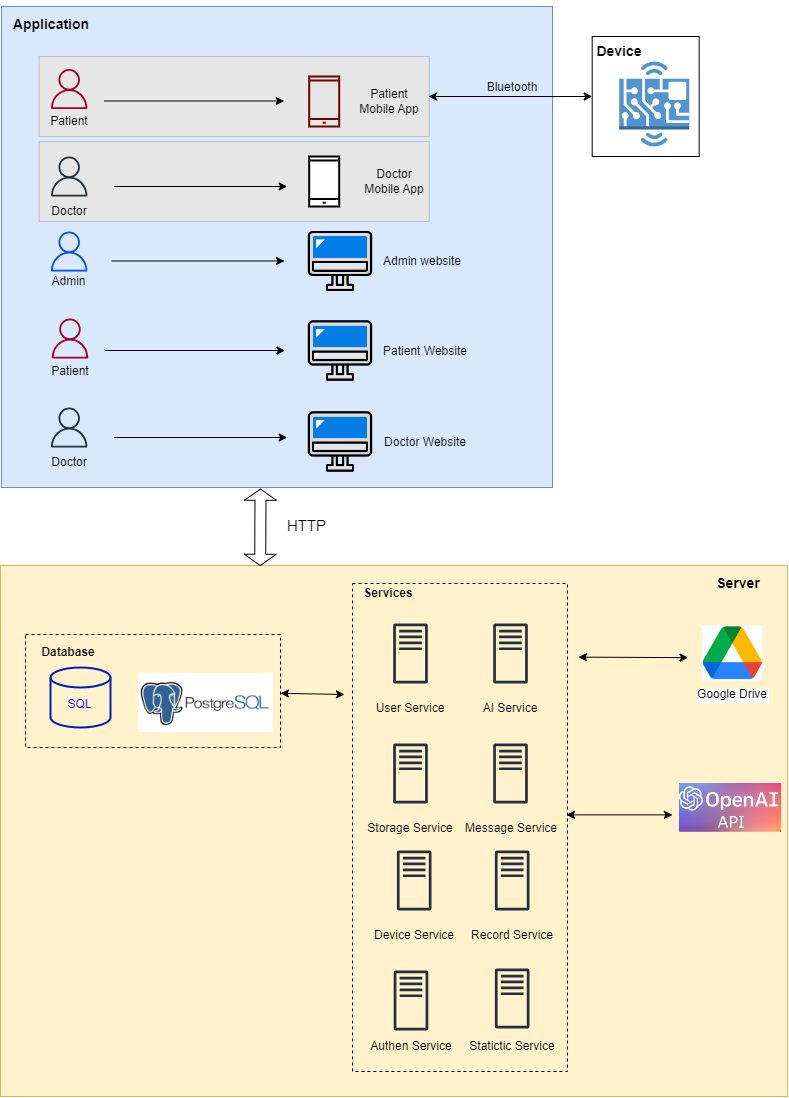
\includegraphics[width=12cm,height=14cm]{Images/system/fmECG_architecture-System_Architecture.png}
  \caption[Kiến trúc tổng quan hệ thống]{\bfseries \fontsize{12pt}{0pt}\selectfont Kiến trúc tổng quan hệ thống}
  \label{fmECG_architecture-System} %đặt tên cho ảnh
\end{figure}

Hình \ref{fmECG_architecture-System} thể hiện ba phần: 

\begin{adjustwidth}{1.5em}{}
\begin{itemize}
  \item Device (Thiết bị): Bao gồm thiết bị phần cứng đo điện tim, có thể kết nối với ứng dụng di động của bệnh nhân thông qua Bluetooth 
  \item Application (Ứng dụng): Bao gồm ứng dụng di động cho bệnh nhân, bác sĩ; website của quản trị viên, website của bác sĩ, website của bệnh nhân
  \item Server (Máy chủ): Bao gồm các Services để xử lý các yêu cầu gửi từ Application, cơ sở dữ liệu, Cloud lưu trữ, kết nối với model GPT-4 trên OpenAI thông qua API
\end{itemize}
\end{adjustwidth}

Trong sơ đồ kiến trúc hệ thống, bệnh nhân tương tác trực tiếp với Thiết bị (Device) thông qua ứng dụng di động (Mobile App). Khối Ứng dụng (Application) giao tiếp với Khối Máy chủ (Server) thông qua API với giao thức HTTP. 
Khi nhận được yêu cầu từ Application, Server sẽ xử lý dữ liệu. Mọi yêu cầu đều được xử lý bởi các Services chuyên biệt. Dựa vào loại yêu cầu, Service tương ứng sẽ lấy hoặc lưu dữ liệu trong cơ sở dữ liệu và trả về kết quả cho người dùng.\begin{adjustwidth}{1.5em}{}
\begin{itemize}
  \item User Service: Xử lý các yêu cầu liên quan đến người dùng như đăng ký, đăng nhập, lấy thông tin cá nhân
  \item Storage Service: Xử lý các tác vụ liên quan tới lưu trữ dữ liệu của hệ thống
  \item AI Service: Xử lý các tác vụ liên quan tới trợ lý ảo, bao gồm: huấn luyện, kết nối với model GPT-4 thông qua api và xử lý kết quả 
  và trả về tin nhắn và các hành động của ai can thiệp trực tiếp vào hệ thống 
  \item Message Service: Xử lý các yêu cầu liên quan tới hội thoại, tin nhắn.
  \item Device Service: Xử lý các tác vụ liên quan tới thiết bị như thêm, sửa, xoá thiết bị, cập nhật thông tin.
  \item Record Service: Xử lý các tác vụ liên quan tới bản ghi như là thêm sửa xoá, xử lý dữ liệu file đo, vẽ đồ thị
  \item Authen Service: Xử lý các tác vụ liên quan tới bảo mật như: mã hoá và cung cấp token, kiểm tra token, phân quyền truy cập api, mã hoá các dữ liệu nhạy cảm trước khi lưu trữ.
  \item Statictic Service: Xử lý các tác vụ liên quan tới thống kê như: thống kê người dùng, thiết bị, bản ghi, tin nhắn theo tuần theo tháng.
\end{itemize}
\end{adjustwidth}

Ngoài ra hệ thống sẽ có thêm chức năng tự động triển khai trên môi trường internet để việc phát triển và kiểm thử dễ dàng 
làm tăng chất lượng và độ hoàn thiện của hệ thống.

Sau đây là mô tả chi tiết về từng khối nhỏ hơn trong kiến trúc hệ thống, dựa trên các đối tượng đã được xác định trong hệ thống.
\newpage
\subsection{Sơ đồ khối phần mềm}

\subsubsection{Website dành cho bệnh nhân}
\mbox{}

\begin{figure}[H]
  \centering
  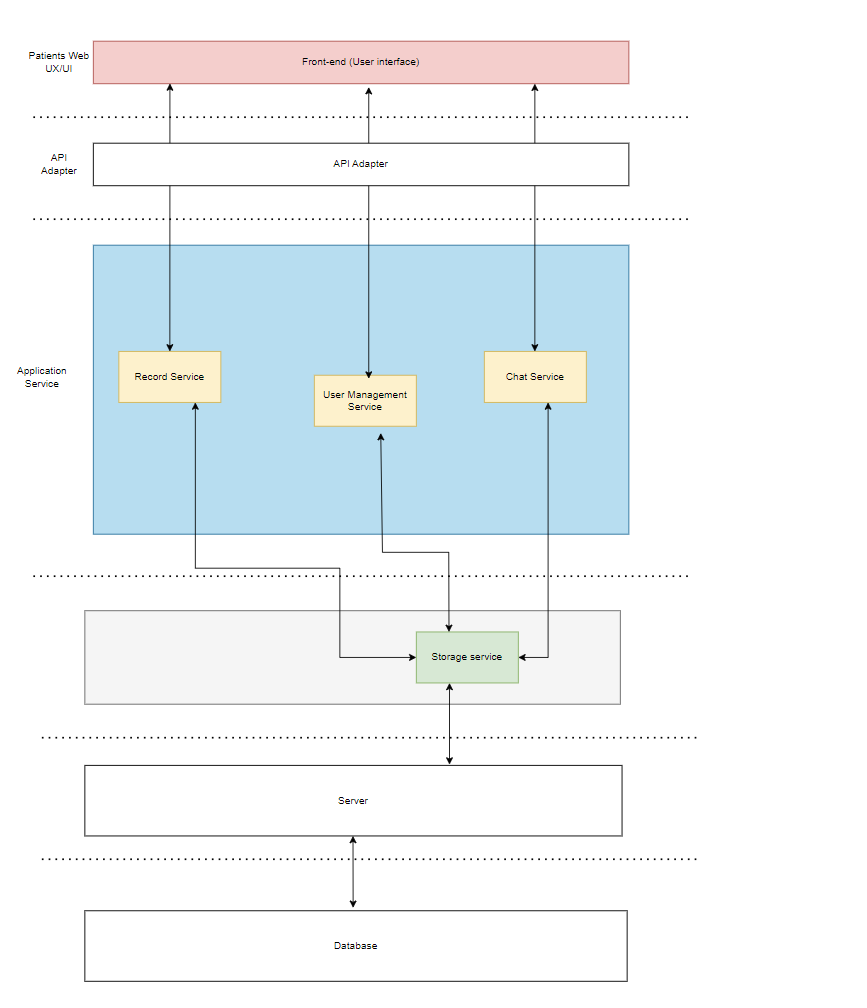
\includegraphics[width=12cm,height=14cm]{Images/system/fmECG_architecture-Patient.drawio.png}
  \caption[Sơ đồ khối Website dành cho bệnh nhân]{\bfseries \fontsize{12pt}{0pt}\selectfont Sơ đồ khối Website dành cho bệnh nhân}
  \label{fmECG_architecture-Patient} %đặt tên cho ảnh
\end{figure}
Lớp trên cùng trong sơ đồ là User Interface (Giao diện người dùng), nơi người dùng tương tác và thực hiện yêu cầu thông qua API Adapter. 
Các yêu cầu này được xử lý bởi Services và kết quả được trả về cho người dùng qua giao diện. Các Service trong khối bao gồm:
\begin{adjustwidth}{1.5em}{}
\begin{itemize}
  \item Record Service: Khối có nhiệm vụ xử lý yêu cầu cho chức năng đo và quản lý bản ghi: thực hiện đo, kết thúc đo, lưu kết quả đo, xử lý kết quả đo và cung cấp dữ liệu để vẽ đồ thị điện tim
  \item User Management Service: Khối có nhiệm vụ xử lý các vấn đề liên quan đến người dùng như đăng nhập, đăng ký, xem thông tin người dùng
  \item Device Service: Khối có nhiệm vụ xử lý các vấn đề liên quan đến thiết bị như thêm sửa xoá, thay đổi thông tin, cung cấp thiết bị cho người dùng
  \item Chat Service: Khối có nhiệm vụ quản lý việc chat, trao đổi thông tin với bác sĩ và trợ lý ảo
  \item Storage Service: Khối có nhiệm vụ lưu thông tin vào bộ nhớ
\end{itemize}
\end{adjustwidth}


\subsubsection{Website dành cho bác sĩ}

\begin{figure}[H]
  \centering
  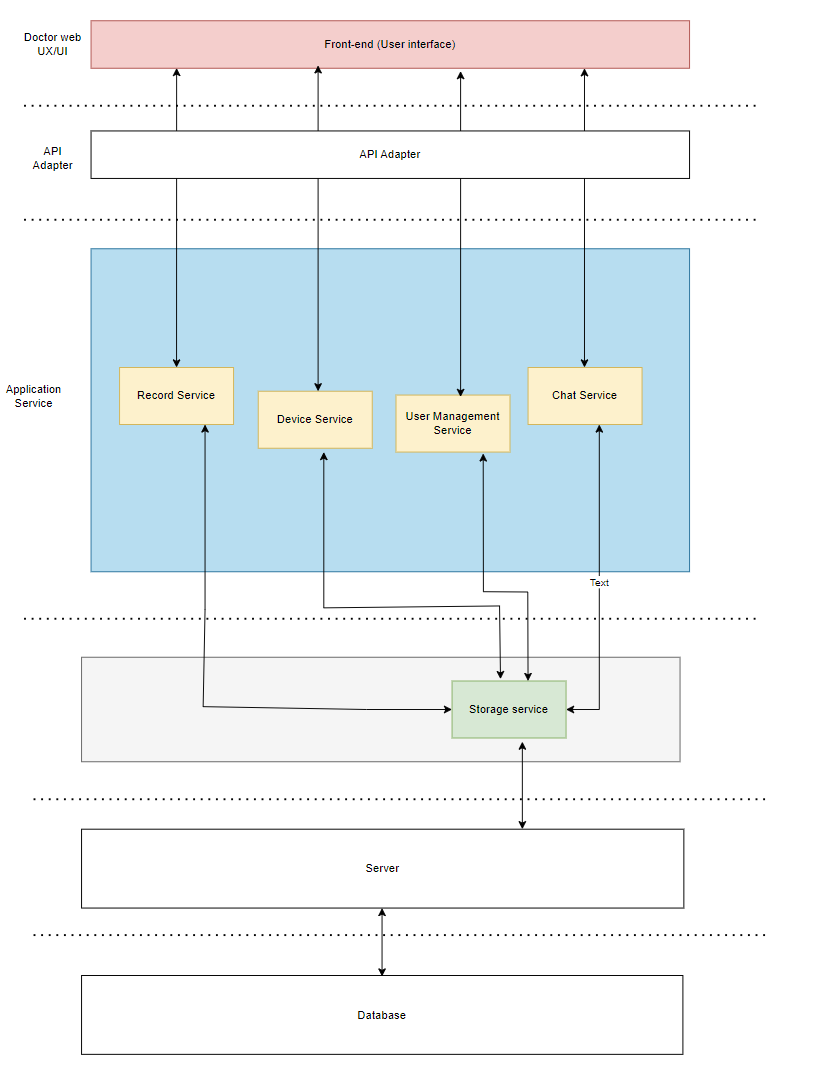
\includegraphics[width=12cm,height=14cm]{Images/system/fmECG_architecture-Doctors.drawio.png}
  \caption[Sơ đồ khối Website dành cho bác sĩ]{\bfseries \fontsize{12pt}{0pt}\selectfont Sơ đồ khối Website dành cho bác sĩ}
  \label{fmECG_architecture-Doctors} %đặt tên cho ảnh
\end{figure}

Về cơ bản, website cho bác sĩ có những khối tương tự với bệnh nhân, trừ việc bác sĩ sẽ có thêm quyền quản lý thiết bị (Device Service)

\subsubsection{Website cho quản trị viên}

\begin{figure}[H]
  \centering
  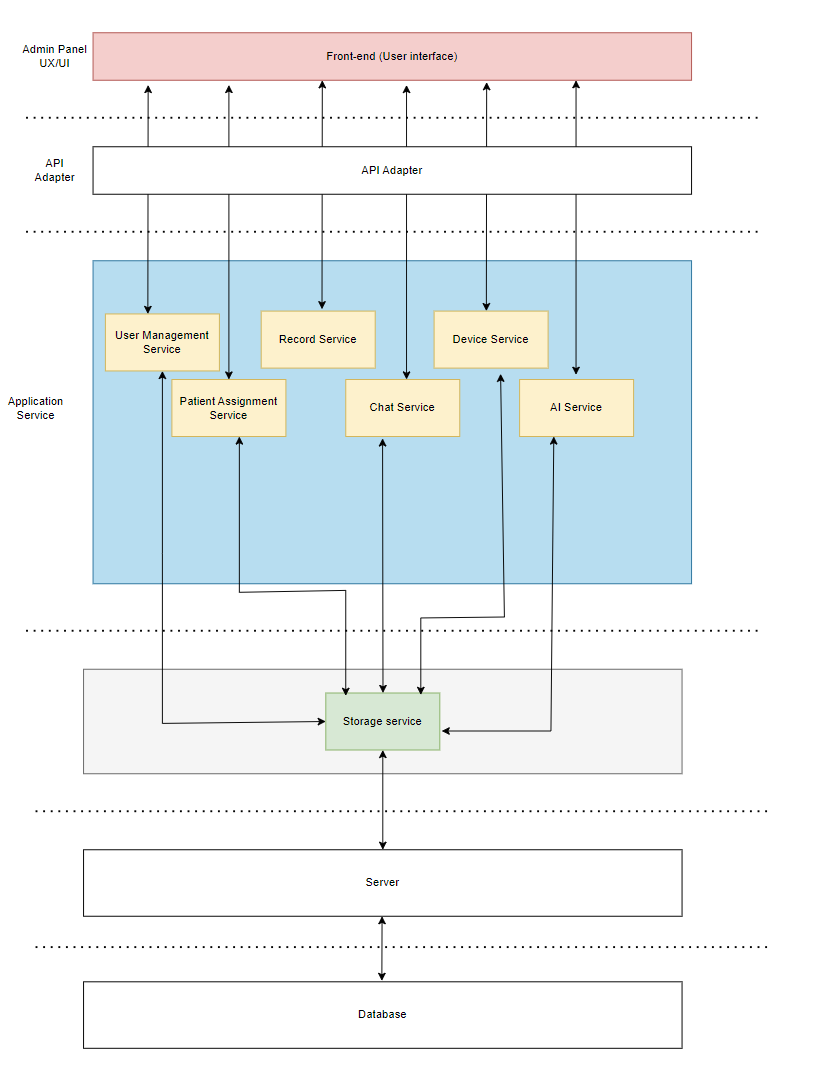
\includegraphics[width=12cm,height=14cm]{Images/system/fmECG_architecture-Admin.drawio.png}
  \caption[Sơ đồ khối Website dành cho quản trị viên]{\bfseries \fontsize{12pt}{0pt}\selectfont Sơ đồ khối Website dành cho quản trị viên}
  \label{fmECG_architecture-Admin} %đặt tên cho ảnh
\end{figure}

Website cho quản trị viên có kiến trúc tương tự với website bệnh nhân và bác sĩ. Các Service trong được quản trị viên quản lý bao gồm quản lý người dùng (User Service), quản lý thiết bị (Device Service), quản lý phân công
bác sĩ - bệnh nhân (Patient Assignment Service), quản lý bản ghi (Record Service), Chat Service, huấn luyện trợ lý ảo (AI service).
 
\newpage

\subsection{Thiết kế cơ sở dữ liệu}
\label{design_database}
\subsubsection{Chuyển mô hình thực thể sang mô hình quan hệ}
Dựa trên phần mô tả các thực thể, chúng em sẽ chuyển mô hình thực thể liên kết sang mô hình quan hệ như sau:

\begin{itemize}
  \item Người dùng (\textbf{ID người dùng}, ID tài khoản, Tên người dùng, Ngày sinh, Giới tính, Số điện thoại, Quyền, Trạng thái, Đường dẫn lưu trữ ảnh đại diện, Thông tin người dùng)
  \item Tài khoản (\textbf{ID tài khoản}, Email, Mật khẩu)
  \item Token đăng nhập (\textbf{ID token}, ID tài khoản, Token truy cập, Token làm mới)
  \item Thiết bị (\textbf{ID thiết bị}, ID người dùng thiết bị, ID bác sĩ theo dõi, Tên thiết bị, Loại thiết bị, Thông tin thiết bị, Trạng thái thiết bị, Ngày bắt đầu sử dụng)
  \item Thông số thiết bị (\textbf{ID thông số}, ID thiết bị, Tên thông số, Giá trị, Thông tin thông số, Loại thông số)
  \item Bản ghi dữ liệu (\textbf{ID bản ghi dữ liệu}, ID người dùng, ID thiết bị, Loại bản ghi, Đường dẫn lưu trữ dữ liệu, Thời gian bắt đầu đo, Thời gian kết thúc đo)
  \item Cuộc hội thoại (\textbf{ID hội thoại}, Tên hội thoại, Loại hội thoại, Đường dẫn avatar hội thoại)
  \item Thành viên tham gia hội thoại (\textbf{ID thành viên}, ID hội thoại, ID người dùng, Trạng thái thông báo, Tác vụ, Trạng thái đã xem)
  \item Tin nhắn (\textbf{ID tin nhắn}, ID hội thoại, ID người gửi, Các tệp đính kèm, Tin nhắn hệ thống, Ghim, Thời gian ghim tin nhắn, Các lượt thả cảm xúc)
  \item Tệp đính kèm (\textbf{ID tệp đính kèm}, ID tin nhắn, ID hội thoại, Đường dẫn nội dung, Tên tệp, Kích thước tệp, Đường dẫn thumbnail, Loại đính kèm)
  \item Phân công bệnh nhân - bác sĩ (\textbf{ID phân công}, ID bệnh nhân, ID bác sĩ, Ngày bắt đầu)
  \item Tài khoản phê duyệt (\textbf{ID tài khoản phê duyệt}, Email, Mật khẩu, Tên người dùng, Ngày sinh, Giới tính, Số điện thoại, Quyền, Trạng thái, Đường dẫn lưu trữ ảnh đại diện, Thông tin người dùng)
\end{itemize}

\subsubsection{Chuẩn hoá 3NF}
Các bảng đã được thiết kế theo nguyên tắc chuẩn hoá 3NF, vì không có thuộc tính lặp lại và các thuộc tính không phụ thuộc vào một tập hợp con của khóa chính.

\paragraph{Chuẩn hoá bảng Người dùng}
\mbox{}
\begin{table}[H]
  \caption{\bfseries \fontsize{12pt}{0pt}\selectfont Bảng chuẩn hoá bảng Người dùng}
  \centering
  \begin{tabularx}{0.9\textwidth}{|X|X|}
    \hline
    \textbf{Danh sách thuộc tính} & ID người dùng, ID tài khoản, Tên người dùng, Ngày sinh, Giới tính, Số điện thoại, Quyền, Trạng thái, Đường dẫn lưu trữ ảnh, Thông tin người dùng \\
    \hline
    \textbf{Quy tắc nghiệp vụ} & \textbf{Phụ thuộc hàm} \\
    \hline
    Mỗi người dùng có một ID riêng, có duy nhất ID tài khoản, tên, ngày sinh, giới tính, số điện thoại, quyền,
    trạng thái, đường dẫn lưu trữ ảnh, thông tin & \parbox[t]{\linewidth}{$\text{ID người dùng} \rightarrow$ ID tài khoản, Tên người dùng, Ngày sinh, Giới Tính, Số điện thoại, Quyền, Trạng thái, Đường dẫn lưu trữ ảnh, Thông tin} \\
    \hline
    \multicolumn{2}{|X|}{$\Rightarrow \text{Khoá chính của bảng: ID người dùng}$} \\
    \multicolumn{2}{|X|}{$\Rightarrow \text{Bảng Người dùng đã ở 3NF}$} \\
    \hline
  \end{tabularx}
\end{table}

\paragraph{Chuẩn hoá bảng Tài khoản}
\mbox{}
\begin{table}[H]
  \caption{\bfseries \fontsize{12pt}{0pt}\selectfont Bảng chuẩn hoá bảng Tài khoản}
  \centering
  \begin{tabularx}{0.9\textwidth}{|X|X|}
    \hline
    \textbf{Danh sách thuộc tính} & ID tài khoản, Email, Mật khẩu \\
    \hline
    \textbf{Quy tắc nghiệp vụ} & \textbf{Phụ thuộc hàm} \\
    \hline
    Mỗi tài khoản có một ID riêng, có duy nhất email, mật khẩu 
    & \parbox[t]{\linewidth}{$\text{ID tài khoản} \rightarrow$ Email, mật khẩu} \\
    \hline
    \multicolumn{2}{|X|}{$\Rightarrow \text{Khoá chính của bảng: ID tài khoản}$} \\
    \multicolumn{2}{|X|}{$\Rightarrow \text{Bảng Tài khoản đã ở 3NF}$} \\
    \hline
  \end{tabularx}
\end{table}

\paragraph{Chuẩn hoá bảng Token đăng nhập}
\mbox{}
\begin{table}[H]
  \caption{\bfseries \fontsize{12pt}{0pt}\selectfont Bảng chuẩn hoá bảng Token đăng nhập}
  \centering
  \begin{tabularx}{0.9\textwidth}{|X|X|}
    \hline
    \textbf{Danh sách thuộc tính} & ID token, ID tài khoản, Token truy cập, Token làm mới \\
    \hline
    \textbf{Quy tắc nghiệp vụ} & \textbf{Phụ thuộc hàm} \\
    \hline
    Mỗi người dùng có một ID token riêng, có duy nhất ID tài khoản, token truy cập và token làm mới 
    & \parbox[t]{\linewidth}{$\text{ID token} \rightarrow$ ID tài khoản, Token truy cập, Token làm mới} \\
    \hline
    \multicolumn{2}{|X|}{$\Rightarrow \text{Khoá chính của bảng: ID token đăng nhập}$} \\
    \multicolumn{2}{|X|}{$\Rightarrow \text{Bảng Token  đã ở 3NF}$} \\
    \hline
  \end{tabularx}
\end{table}

\paragraph{Chuẩn hoá bảng Thiết bị}
\mbox{}
\begin{table}[H]
  \caption{\bfseries \fontsize{12pt}{0pt}\selectfont Bảng chuẩn hoá bảng Thiết bị}
  \centering
  \begin{tabularx}{0.9\textwidth}{|X|X|}
    \hline
    \textbf{Danh sách thuộc tính} & ID thiết bị, ID người dùng thiết bị, ID bác sĩ theo dõi, Tên thiết bị, 
    Loại thiết bị, Thông tin thiết bị, Trạng thái thiết bị, Ngày bắt đầu sử dụng \\
    \hline
    \textbf{Quy tắc nghiệp vụ} & \textbf{Phụ thuộc hàm} \\
    \hline
    Mỗi thiết bị khi được sử dụng sẽ có một ID thiết bị riêng, có duy nhất tên thiết bị, loại thiết bị, thông tin thiết bị.
    ID người dùng thiết bị, ID bác sĩ theo dõi, trạng thái thiết bị, ngày bắt đầu sử dụng
    & \parbox[t]{\linewidth}{$\text{ID thiết bị} \rightarrow$ ID người dùng thiết bị, ID bác sĩ theo dõi, Tên thiết bị, 
    Loại thiết bị, Thông tin thiết bị, Trạng thái thiết bị, Ngày bắt đầu sử dụng} \\
    \hline
    \multicolumn{2}{|X|}{$\Rightarrow \text{Khoá chính của bảng: ID thiết bị}$} \\
    \multicolumn{2}{|X|}{$\Rightarrow \text{Bảng Thiết bị đã ở 3NF}$} \\
    \hline
  \end{tabularx}
\end{table}

\paragraph{Chuẩn hoá bảng Thông số thiết bị}
\mbox{}
\begin{table}[H]
  \caption{\bfseries \fontsize{12pt}{0pt}\selectfont Bảng chuẩn hoá bảng Thông số thiết bị}
  \centering
  \begin{tabularx}{0.9\textwidth}{|X|X|}
    \hline
    \textbf{Danh sách thuộc tính} & ID thông số, ID thiết bị, Tên thông số, Giá trị, 
    Thông tin thông số, Loại thông số \\
    \hline
    \textbf{Quy tắc nghiệp vụ} & \textbf{Phụ thuộc hàm} \\
    \hline
    Mỗi thông số thiết bị sẽ có một ID thông số riêng, có duy nhất Tên thông số, ID thiết bị, Giá trị,
    Thông tin thông số, Loại thông số
    & \parbox[t]{\linewidth}{$\text{ID thông số} \rightarrow$ Tên thông số, ID thiết bị, Giá trị,
    Thông tin thông số, Loại thông số} \\
    \hline
    \multicolumn{2}{|X|}{$\Rightarrow \text{Khoá chính của bảng: ID thông số thiết bị}$} \\
    \multicolumn{2}{|X|}{$\Rightarrow \text{Bảng Thiết bị đã ở 3NF}$} \\
    \hline
  \end{tabularx}
\end{table}

\paragraph{Chuẩn hoá bảng Bản ghi dữ liệu}
\mbox{}
\begin{table}[H]
  \caption{\bfseries \fontsize{12pt}{0pt}\selectfont Bảng chuẩn hoá bảng Bản ghi dữ liệu}
  \centering
  \begin{tabularx}{0.9\textwidth}{|X|X|}
    \hline
    \textbf{Danh sách thuộc tính} & ID bản ghi dữ liệu, ID người dùng, ID thiết bị, Loại bản ghi, 
    Đường dẫn lưu trữ dữ liệu, Thời gian bắt đầu đo, Thời gian kết thúc đo \\
    \hline
    \textbf{Quy tắc nghiệp vụ} & \textbf{Phụ thuộc hàm} \\
    \hline
    Mỗi bản ghi có một ID bản ghi dữ liệu riêng, có duy nhất ID người dùng, ID thiết bị, Loại bản ghi, 
    Đường dẫn lưu trữ dữ liệu, Thời gian bắt đầu đo, Thời gian kết thúc đo
    & \parbox[t]{\linewidth}{$\text{ID bản ghi dữ liệu} \rightarrow$ ID người dùng, ID thiết bị, Loại bản ghi, 
    Đường dẫn lưu trữ dữ liệu, Thời gian bắt đầu đo, Thời gian kết thúc đo} \\
    \hline
    \multicolumn{2}{|X|}{$\Rightarrow \text{Khoá chính của bảng: ID bản ghi dữ liệu}$} \\
    \multicolumn{2}{|X|}{$\Rightarrow \text{Bảng Bản ghi dữ liệu đã ở 3NF}$} \\
    \hline
  \end{tabularx}
\end{table}

\paragraph{Chuẩn hoá bảng Thông tin hội thoại}
\mbox{}
\begin{table}[H]
  \caption{\bfseries \fontsize{12pt}{0pt}\selectfont Bảng chuẩn hoá bảng Thông tin hội thoại}
  \centering
  \begin{tabularx}{0.9\textwidth}{|X|X|}
    \hline
    \textbf{Danh sách thuộc tính} & ID hội thoại, Tên hội thoại, 
    Loại hội thoại, Đường dẫn avatar hội thoại \\
    \hline
    \textbf{Quy tắc nghiệp vụ} & \textbf{Phụ thuộc hàm} \\
    \hline
    Mỗi hội thoại có một ID hội thoại riêng, có duy nhất tên hội thoại, 
    loại hội thoại, đường dẫn avatar hội thoại
    & \parbox[t]{\linewidth}{$\text{ID hội thoại} \rightarrow$ Tên hội thoại, 
    Loại hội thoại, Đường dẫn avatar hội thoại} \\
    \hline
    \multicolumn{2}{|X|}{$\Rightarrow \text{Khoá chính của bảng: ID hội thoại}$} \\
    \multicolumn{2}{|X|}{$\Rightarrow \text{Bảng Thông tin hội thoại đã ở 3NF}$} \\
    \hline
  \end{tabularx}
\end{table}

\paragraph{Chuẩn hoá bảng Thành viên tham gia hội thoại}
\mbox{}
\begin{table}[H]
  \caption{\bfseries \fontsize{12pt}{0pt}\selectfont Bảng chuẩn hoá bảng Thành viên tham gia hội thoại}
  \centering
  \begin{tabularx}{0.9\textwidth}{|X|X|}
    \hline
    \textbf{Danh sách thuộc tính} & ID, ID hội thoại, ID người dùng tham gia,
    Trạng thái thông báo, Tác vụ, Trạng thái đã xem \\
    \hline
    \textbf{Quy tắc nghiệp vụ} & \textbf{Phụ thuộc hàm} \\
    \hline
    Mỗi hội thoại có nhiều ID người dùng tham gia, mỗi người dùng có duy nhất trạng thái thông báo,
    tác vụ, trạng thái đã xem trong một hội thoại
    & \parbox[t]{\linewidth}{$\text{ID} \rightarrow$ ID hội thoại, ID người dùng tham gia,
    Trạng thái thông báo, Tác vụ, Trạng thái đã xem} \\
    \hline
    \multicolumn{2}{|X|}{$\Rightarrow \text{Khoá chính của bảng: ID}$} \\
    \multicolumn{2}{|X|}{$\Rightarrow \text{Bảng Thành viên tham gia hội thoại đã ở 3NF}$} \\
    \hline
  \end{tabularx}
\end{table}

\paragraph{Chuẩn hoá bảng Tin nhắn}
\mbox{}
\begin{table}[H]
  \caption{\bfseries \fontsize{12pt}{0pt}\selectfont Bảng chuẩn hoá bảng Tin nhắn}
  \centering
  \begin{tabularx}{0.9\textwidth}{|X|X|}
    \hline
    \textbf{Danh sách thuộc tính} & ID tin nhắn, ID hội thoại, ID người gửi, Các tệp đính kèm, 
    Tin nhắn hệ thống, Ghim, Thời gian ghim tin nhắn, Các lượt thả cảm xúc \\
    \hline
    \textbf{Quy tắc nghiệp vụ} & \textbf{Phụ thuộc hàm} \\
    \hline
    Mỗi tin nhắn có một ID tin nhắn riêng, thuộc một hội thoại, có duy nhất ID người gửi, các tệp đính kèm,
    tin nhắn hệ thống, ghim, thời gian ghim tin nhắn, các lượt thả cảm xúc
    & \parbox[t]{\linewidth}{$\text{ID tin nhắn} \rightarrow$ ID hội thoại, ID người gửi, các tệp đính kèm,
    tin nhắn hệ thống, ghim, thời gian ghim tin nhắn, các lượt thả cảm xúc} \\
    \hline
    \multicolumn{2}{|X|}{$\Rightarrow \text{Khoá chính của bảng: ID tin nhắn}$} \\
    \multicolumn{2}{|X|}{$\Rightarrow \text{Bảng Tin nhắn đã ở 3NF}$} \\
    \hline
  \end{tabularx}
\end{table}

\paragraph{Chuẩn hoá bảng Tệp đính kèm}
\mbox{}
\begin{table}[H]
  \caption{\bfseries \fontsize{12pt}{0pt}\selectfont Bảng chuẩn hoá bảng Tệp đính kèm}
  \centering
  \begin{tabularx}{0.9\textwidth}{|X|X|}
    \hline
    \textbf{Danh sách thuộc tính} & ID tệp đính kèm, ID tin nhắn, ID hội thoại, Đường dẫn nội
    dung, Tên tệp, Kích thước tệp, Đường dẫn thumbnail, Loại đính kèm \\
    \hline
    \textbf{Quy tắc nghiệp vụ} & \textbf{Phụ thuộc hàm} \\
    \hline
    Mỗi tệp đính kèm có một ID tệp đính kèm riêng, thuộc một tin nhắn trong một hội thoại, có duy nhất đường dẫn nội
    dung, tên tệp, kích thước tệp, đường dẫn thumbnail, loại đính kèm
    & \parbox[t]{\linewidth}{$\text{ID tệp đính kèm} \rightarrow$ ID tin nhắn, ID hội thoại, Đường dẫn nội
    dung, Tên tệp, Kích thước tệp, Đường dẫn thumbnail, Loại đính kèm} \\
    \hline
    \multicolumn{2}{|X|}{$\Rightarrow \text{Khoá chính của bảng: ID tệp đính kèm}$} \\
    \multicolumn{2}{|X|}{$\Rightarrow \text{Bảng Tệp đính kèm đã ở 3NF}$} \\
    \hline
  \end{tabularx}
\end{table}

\paragraph{Chuẩn hoá bảng Phân công bệnh nhân - bác sĩ}
\mbox{}
\begin{table}[H]
  \caption{\bfseries \fontsize{12pt}{0pt}\selectfont Bảng chuẩn hoá bảng Phân công bệnh nhân - bác sĩ}
  \centering
  \begin{tabularx}{0.9\textwidth}{|X|X|}
    \hline
    \textbf{Danh sách thuộc tính} & ID phân công, ID bệnh nhân, ID bác sĩ, Ngày bắt đầu \\
    \hline
    \textbf{Quy tắc nghiệp vụ} & \textbf{Phụ thuộc hàm} \\
    \hline
    Mỗi phân công bệnh nhân - bác sĩ có một ID phân công riêng, có duy nhất ID bệnh nhân, ID bác sĩ, ngày bắt đầu.
    Mỗi bệnh nhân thuộc một phân công duy nhất, còn mỗi bác sĩ có thể được giao nhiều phân công.
    & \parbox[t]{\linewidth}{$\text{ID phân công} \rightarrow$ ID bệnh nhân, ID bác sĩ, Ngày bắt đầu} \\
    \hline
    \multicolumn{2}{|X|}{$\Rightarrow \text{Khoá chính của bảng: ID phân công}$} \\
    \multicolumn{2}{|X|}{$\Rightarrow \text{Bảng Phân công bệnh nhân - bác sĩ đã ở 3NF}$} \\
    \hline
  \end{tabularx}
\end{table}

\paragraph{Chuẩn hoá bảng Tài khoản phê duyệt}
\mbox{}
\begin{table}[H]
  \caption{\bfseries \fontsize{12pt}{0pt}\selectfont Bảng chuẩn hoá bảng Tài khoản phê duyệt}
  \centering
  \begin{tabularx}{0.9\textwidth}{|X|X|}
    \hline
    \textbf{Danh sách thuộc tính} & ID tài khoản phê duyệt, Email, Mật khẩu, Tên người dùng, Ngày sinh, Giới tính, Số điện thoại, Quyền, Trạng thái, Đường dẫn lưu trữ ảnh, Thông tin người dùng \\
    \hline
    \textbf{Quy tắc nghiệp vụ} & \textbf{Phụ thuộc hàm} \\
    \hline
    Mỗi tài khoản chờ phê duyệt có một ID riêng, có duy nhất Email, Mật khẩu, Tên người dùng, Ngày sinh, Giới tính,
     Số điện thoại, Quyền, Trạng thái, Đường dẫn lưu trữ ảnh, Thông tin người dùng 
    & \parbox[t]{\linewidth}{$\text{ID tài khoản phê duyệt} \rightarrow$ Email, Mật khẩu, Tên người dùng, Ngày sinh, Giới tính,
    Số điện thoại, Quyền, Trạng thái, Đường dẫn lưu trữ ảnh, Thông tin người dùng} \\
    \hline
    \multicolumn{2}{|X|}{$\Rightarrow \text{Khoá chính của bảng: ID tài khoản phê duyệt}$} \\
    \multicolumn{2}{|X|}{$\Rightarrow \text{Bảng Người dùng đã ở 3NF}$} \\
    \hline
  \end{tabularx}
\end{table}

\subsubsection{Từ điển dữ liệu}

\begin{table}[H]
  \caption{\bfseries \fontsize{12pt}{0pt}\selectfont Bảng user}
  \centering
  \begin{tabularx}{\textwidth}{|c|c|X|}
    \hline
    \textbf{Thuộc tính} & \textbf{Kiểu dữ liệu} & \textbf{Mô tả} \\
    \hline
    id & STRING & ID người dùng.  \\
    \hline
    account\_id & STRING & ID tài khoản người dùng. \\
    \hline
    username & STRING & Họ và tên người dùng. \\
    \hline
    gender & INT & Giới tính của người dùng. \\
    \hline
    birth & DATE & Ngày tháng năm sinh của người dùng. \\
    \hline
    phone\_number & STRING & Số điện thoại của người dùng. \\
    \hline
    image & STRING & Ảnh đại diện của người dùng. \\
    \hline
    status & INTEGER & Trạng thái sử dụng của người dùng (0 - còn đang sử dụng, 1 - không còn đang sử dụng). \\
    \hline
    information & STRING & Thông tin thêm về người dùng. \\
    \hline
    role & INTEGER & Chức vụ của người dùng (0 - bệnh nhân, 1 - bác sĩ, 2 - quản trị viên). \\
    \hline
    created\_at & DATE & Thời gian lúc tạo mới dữ liệu trong cơ sở dữ liệu. \\
    \hline
    updated\_at & DATE & Thời gian lúc thay đổi dữ liệu trong cơ sở dữ liệu. \\
    \hline
    
  \end{tabularx}
\end{table}


\begin{table}[H]
  \caption{\bfseries \fontsize{12pt}{0pt}\selectfont Bảng account}
  \centering
  \begin{tabularx}{\textwidth}{|c|c|X|}
    \hline
    \textbf{Thuộc tính} & \textbf{Kiểu dữ liệu} & \textbf{Mô tả} \\
    \hline
    id & STRING & ID tài khoản  \\
    \hline
    email & STRING & Địa chỉ email của tài khoản. \\
    \hline
    password & STRING & Mật khẩu của tài khoản. \\
    \hline
  \end{tabularx}
\end{table}

\begin{table}[H]
  \caption{\bfseries \fontsize{12pt}{0pt}\selectfont Bảng register}
  \centering
  \begin{tabularx}{\textwidth}{|c|c|X|}
    \hline
    \textbf{Thuộc tính} & \textbf{Kiểu dữ liệu} & \textbf{Mô tả} \\
    \hline
    id & STRING & ID tài khoản đăng ký \\
    \hline
    email & STRING & Địa chỉ email của tài khoản đăng ký. \\
    \hline
    password & STRING & Mật khẩu của tài khoản đâng ký. \\
    \hline
    username & STRING & Họ và tên của tài khoản đăng ký. \\
    \hline
    gender & INT & Giới tính của tài khoản đăng ký. \\
    \hline
    birth & DATE & Ngày sinh của tài khoản đăng ký. \\
    \hline
    phone\_number & STRING & Số điện thoại của tài khoản đăng ký. \\
    \hline
    image & STRING & Ảnh đại diện của tài khoản đăng ký. \\
    \hline
    status & INTEGER & Trạng thái của tài khoản đăng ký (0 - đang chờ xử lý, 1 - được admin chấp nhận, 2 - bị admin từ chối). \\
    \hline
    information & STRING & Thông tin thêm về người dùng. \\
    \hline
    role & INTEGER & Chức vụ của tài khoản đăng ký (0 - bệnh nhân, 1 - bác sĩ, 2 - quản trị viên).\\
    \hline
  \end{tabularx}
\end{table}

\begin{table}[H]
  \caption{\bfseries \fontsize{12pt}{0pt}\selectfont Bảng record}
  \centering
  \begin{tabularx}{\textwidth}{|c|c|X|}
    \hline
    \textbf{Thuộc tính} & \textbf{Kiểu dữ liệu} & \textbf{Mô tả} \\
    \hline
    id & STRING & ID bản ghi record  \\
    \hline
    user\_id & STRING & ID bệnh nhân  \\
    \hline
    device\_id & STRING & ID thiết bị theo dõi  \\
    \hline
    record\_type & INTEGER & Loại bản ghi (0 - PPG, 1 - PCG, 2 - HeartRate, 3 - ECG). \\
    \hline
    data\_rec\_url & STRING & Đường dẫn lưu trữ bản ghi. \\
    \hline
    start\_time & DATE & Thời gian bắt đầu phiên đo. \\
    \hline
    end\_time & DATE & Thời gian kết thúc phiên đo. \\
    \hline
    created\_at & DATE & Thời gian lúc tạo mới dữ liệu trong cơ sở dữ liệu. \\
    \hline
    updated\_at & DATE & Thời gian lúc thay đổi dữ liệu trong cơ sở dữ liệu. \\
    \hline
  \end{tabularx}
\end{table}

\begin{table}[H]
  \caption{\bfseries \fontsize{12pt}{0pt}\selectfont Bảng patient\_doctor\_assignment}
  \centering
  \begin{tabularx}{\textwidth}{|c|c|X|}
    \hline
    \textbf{Thuộc tính} & \textbf{Kiểu dữ liệu} & \textbf{Mô tả} \\
    \hline
    id & STRING & ID phân công bác sĩ - bệnh nhân  \\
    \hline
    patient\_id & STRING & ID bệnh nhân  \\
    \hline
    doctor\_id & INTEGER & ID bác sĩ  \\
    \hline
    start\_date & DATE & Ngày bắt đầu phân công. \\
    \hline
    end\_date & DATE & Ngày kết thúc phân công. \\
    \hline
    created\_at & DATE & Thời gian lúc tạo mới dữ liệu trong cơ sở dữ liệu. \\
    \hline
    updated\_at & DATE & Thời gian lúc thay đổi dữ liệu trong cơ sở dữ liệu. \\
    \hline
  \end{tabularx}
\end{table}

\begin{table}[H]
  \caption{\bfseries \fontsize{12pt}{0pt}\selectfont Bảng token}
  \centering
  \begin{tabularx}{\textwidth}{|c|c|X|}
    \hline
    \textbf{Thuộc tính} & \textbf{Kiểu dữ liệu} & \textbf{Mô tả} \\
    \hline
    id & STRING & ID của mã đại diện xác thực  \\
    \hline
    account\_id & STRING & ID tài khoản  \\
    \hline
    access\_token & STRING & Mã đại diện cho người dùng thao tác với hệ thống. \\
    \hline
    refresh\_token & STRING & Mã đại diện cho người dùng thao tác với hệ thống sau khi \texttt{access\_token} hết hạn. \\
    \hline
    created\_at & DATE & Thời gian lúc tạo mới dữ liệu trong cơ sở dữ liệu.. \\
    \hline
    updated\_at & DATE & Thời gian lúc thay đổi dữ liệu trong cơ sở dữ liệu.. \\
    \hline
  \end{tabularx}
\end{table}




\begin{table}[H]
  \caption{\bfseries \fontsize{12pt}{0pt}\selectfont Bảng device}
  \centering
  \begin{tabularx}{\textwidth}{|c|c|X|}
    \hline
    \textbf{Thuộc tính} & \textbf{Kiểu dữ liệu} & \textbf{Mô tả} \\
    \hline
    id & STRING & ID thiết bị  \\
    \hline
    user\_id & STRING & ID bệnh nhân  \\
    \hline
    doctor\_id & STRING & ID bác sĩ  \\
    \hline
    device\_name & STRING & Tên thiết bị. \\
    \hline
    information & STRING & Thông tin thêm về thiết bị. \\
    \hline
    device\_type & INTEGER & Loại thiết bị (1 - thiết bị đo điện tim, 2 - thiết bị đo nhịp tim, âm thanh tim). \\
    \hline
    start\_date & DATE & Thời gian lúc bắt đầu sử dụng thiết bị. \\
    \hline
    status & INTEGER & Trạng thái của thiết bị (0 - đang được sử dụng, 1 - đang không được sử dụng). \\
    \hline
    created\_at & DATE & Thời gian lúc tạo mới dữ liệu trong cơ sở dữ liệu. \\
    \hline
    updated\_at & DATE & Thời gian lúc thay đổi dữ liệu trong cơ sở dữ liệu. \\
    \hline
  \end{tabularx}
\end{table}


\begin{table}[H]
  \caption{\bfseries \fontsize{12pt}{0pt}\selectfont Bảng device\_detail}
  \centering
  \begin{tabularx}{\textwidth}{|c|c|X|}
    \hline
    \textbf{Thuộc tính} & \textbf{Kiểu dữ liệu} & \textbf{Mô tả} \\
    \hline
    id & STRING & ID thông số thiết bị  \\
    \hline
    device\_id & STRING & ID thiết bị  \\
    \hline
    detail\_name & STRING & Tên trường thông số thiết bị dựa vào \texttt{detail\_type}. \\
    \hline
    infomation & STRING & Thông tin về trường \texttt{detail\_name} của thiết bị. \\
    \hline
    value & STRING & Giá trị thông số của thiết bị dựa vào \texttt{detail\_type} (1 - tần số, 2 - dữ liệu kết nối, 3 - dung lượng lưu trữ). \\
    \hline
    detail\_type & INTEGER & Loại thông tin về thiết bị (1 - tín hiệu đo, 2 - loại kết nối, 3 - kiểu lưu trữ). \\
    \hline
    created\_at & DATE & Thời gian lúc tạo mới dữ liệu trong cơ sở dữ liệu. \\
    \hline
    updated\_at & DATE & Thời gian lúc thay đổi dữ liệu trong cơ sở dữ liệu. \\
    \hline
  \end{tabularx}
\end{table}

\begin{table}[H]
  \caption{\bfseries \fontsize{12pt}{0pt}\selectfont Bảng conversation}
  \centering
  \begin{tabularx}{\textwidth}{|c|c|X|}
    \hline
    \textbf{Thuộc tính} & \textbf{Kiểu dữ liệu} & \textbf{Mô tả} \\
    \hline
    conversation\_id & STRING & ID cuộc hội thoại  \\
    \hline
    name & STRING & Tên cuộc hội thoại \\
    \hline
    type & INTEGER & Loại cuộc hội thoại (0 - hội thoại 2 người, 1 - hội thoại nhóm, 2 - chatbot) \\
    \hline
    avatar & STRING & Đường dẫn ảnh đại diện của cuộc hội thoại  \\
    \hline
    created\_at & DATE & Thời gian lúc tạo mới dữ liệu trong cơ sở dữ liệu \\
    \hline
    updated\_at & DATE & Thời gian lúc thay đôi dữ liệu trong cơ sở dữ liệu \\
    \hline
  \end{tabularx}
\end{table}

\begin{table}[H]
  \caption{\bfseries \fontsize{12pt}{0pt}\selectfont Bảng message}
  \centering
  \begin{tabularx}{\textwidth}{|c|c|X|}
    \hline
    \textbf{Thuộc tính} & \textbf{Kiểu dữ liệu} & \textbf{Mô tả} \\
    \hline
    message\_id & STRING & ID tin nhắn  \\
    \hline
    conversation\_id & STRING & ID hội thoại  \\
    \hline
    sender\_id & STRING & ID người gửi tin nhắn  \\
    \hline
    attachments & LIST <Map> & Danh sách tệp tin đính kèm khi gửi tin nhắn\\
    \hline
    system\_message & BOOLEAN & Tin nhắn trả về từ hệ thống\\
    \hline
    pin & BOOLEAN & Đánh dấu tin nhắn có được ghim không\\
    \hline
    pin\_time & DATE & Thời gian ghim tin nhắn\\
    \hline
    reactions & LIST <Map> & Danh sách các phản ứng lại với tin nhắn này.\\
    \hline
    created\_at & DATE & Thời gian lúc tạo mới dữ liệu trong cơ sở dữ liệu \\
    \hline
    updated\_at & DATE & Thời gian lúc thay đổi dữ liệu trong cơ sở dữ liệu \\
    \hline
  \end{tabularx}
\end{table}

\begin{table}[H]
  \caption{\bfseries \fontsize{12pt}{0pt}\selectfont Bảng conversation\_member}
  \centering
  \begin{tabularx}{\textwidth}{|c|c|X|}
    \hline
    \textbf{Thuộc tính} & \textbf{Kiểu dữ liệu} & \textbf{Mô tả} \\
    \hline
    id & STRING & ID của thành viên hội thoại \\
    \hline
    conversation\_id & STRING & ID hội thoại \\
    \hline
    user\_id & STRING & ID người dùng  \\
    \hline
    status\_notify & INTEGER & Trạng thái thông báo tin nhắn (0 - có thông báo tin nhắn, 1 - không nhận thông báo tin nhắn).\\
    \hline
    seen & BOOLEAN & Tin nhắn đã được xem chưa.\\
    \hline
    role & INTEGER & Vai trò của người dùng trong hội thoại (tương ứng trong bảng \texttt{user}).\\
    \hline
    created\_at & DATE & Thời gian lúc tạo mới dữ liệu trong cơ sở dữ liệu \\
    \hline
    updated\_at & DATE & Thời gian lúc thay đổi dữ liệu trong cơ sở dữ liệu \\
    \hline
  \end{tabularx}
\end{table}


\begin{table}[H]
  \caption{\bfseries \fontsize{12pt}{0pt}\selectfont Bảng conversation\_attachment}
  \centering
  \begin{tabularx}{\textwidth}{|c|c|X|}
    \hline
    \textbf{Thuộc tính} & \textbf{Kiểu dữ liệu} & \textbf{Mô tả} \\
    \hline
    id & STRING & ID tệp đính kèm tin nhắn  \\
    \hline
    conversation\_id & STRING & ID cuộc hội thoại  \\
    \hline
    message\_id & STRING & ID tin nhắn  \\
    \hline
    content\_url & STRING & Đường dẫn lưu trữ tệp đính kèm\\
    \hline
    file\_name & STRING & Tên của tệp tin.\\
    \hline
    size & INTEGER & Dung lượng của tệp tin.\\
    \hline
    thumbnail\_url & STRING & Đoạn mã chứa hình ảnh tĩnh của tệp tin.\\
    \hline
    type & INTEGER & Loại của tệp tin (0 - ảnh, 1 - video, 2 - tệp). \\
    \hline
    created\_at & DATE & Thời gian lúc tạo mới dữ liệu trong cơ sở dữ liệu \\
    \hline
    updated\_at & DATE & Thời gian lúc thay đổi dữ liệu trong cơ sở dữ liệu \\
    \hline
  \end{tabularx}
\end{table}

\subsubsection{Sơ đồ ERD}

\begin{figure}[H]
  \centering
  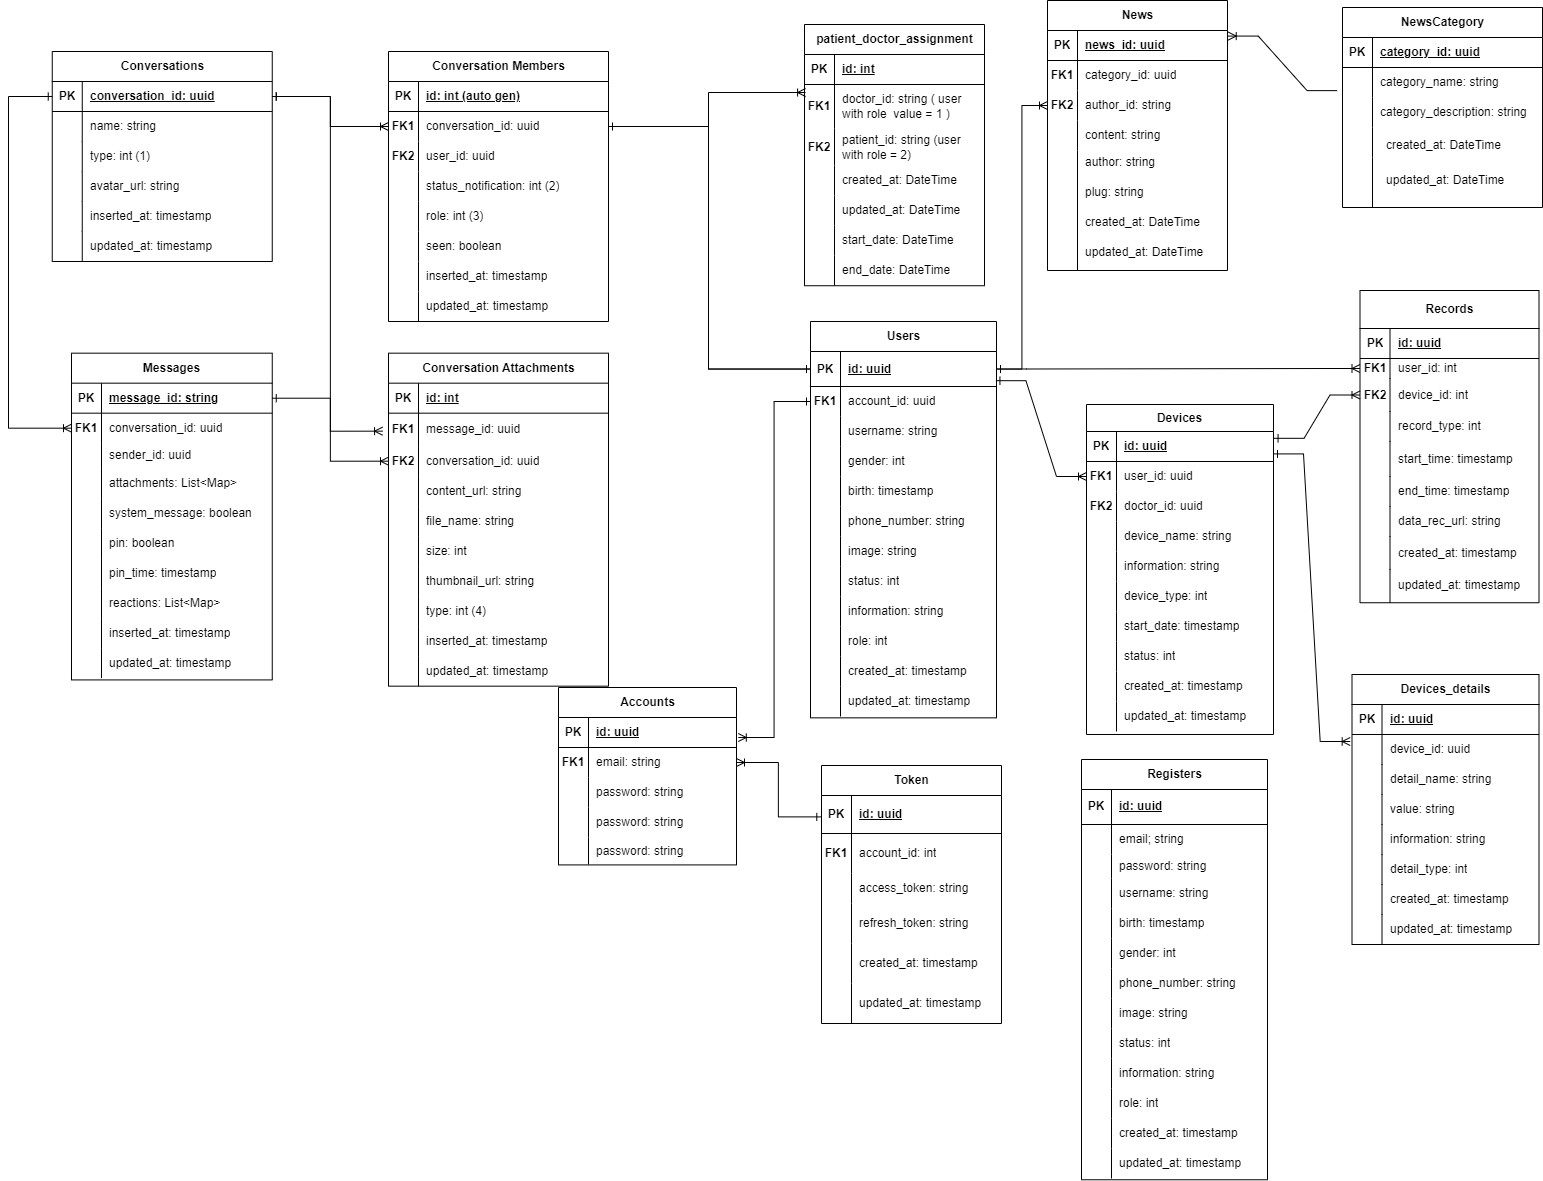
\includegraphics[width=15cm,height=15cm]{Images/system/fmECG_database.png}
  \caption[Sơ đồ ERD]{\bfseries \fontsize{12pt}{0pt}\selectfont Sơ đồ ERD}
  \label{fmECG_architecture-Database} %đặt tên cho ảnh
\end{figure}

\subsection{Thiết kế giao diện}

Sau khi thiết kế cơ sơ dữ liệu cho hệ thống, bước tiếp theo cho việc thiết kế hệ thống là thiết kế giao diện website quản trị cùng các chức năng. 
\begin{figure}[H]
  \centering
  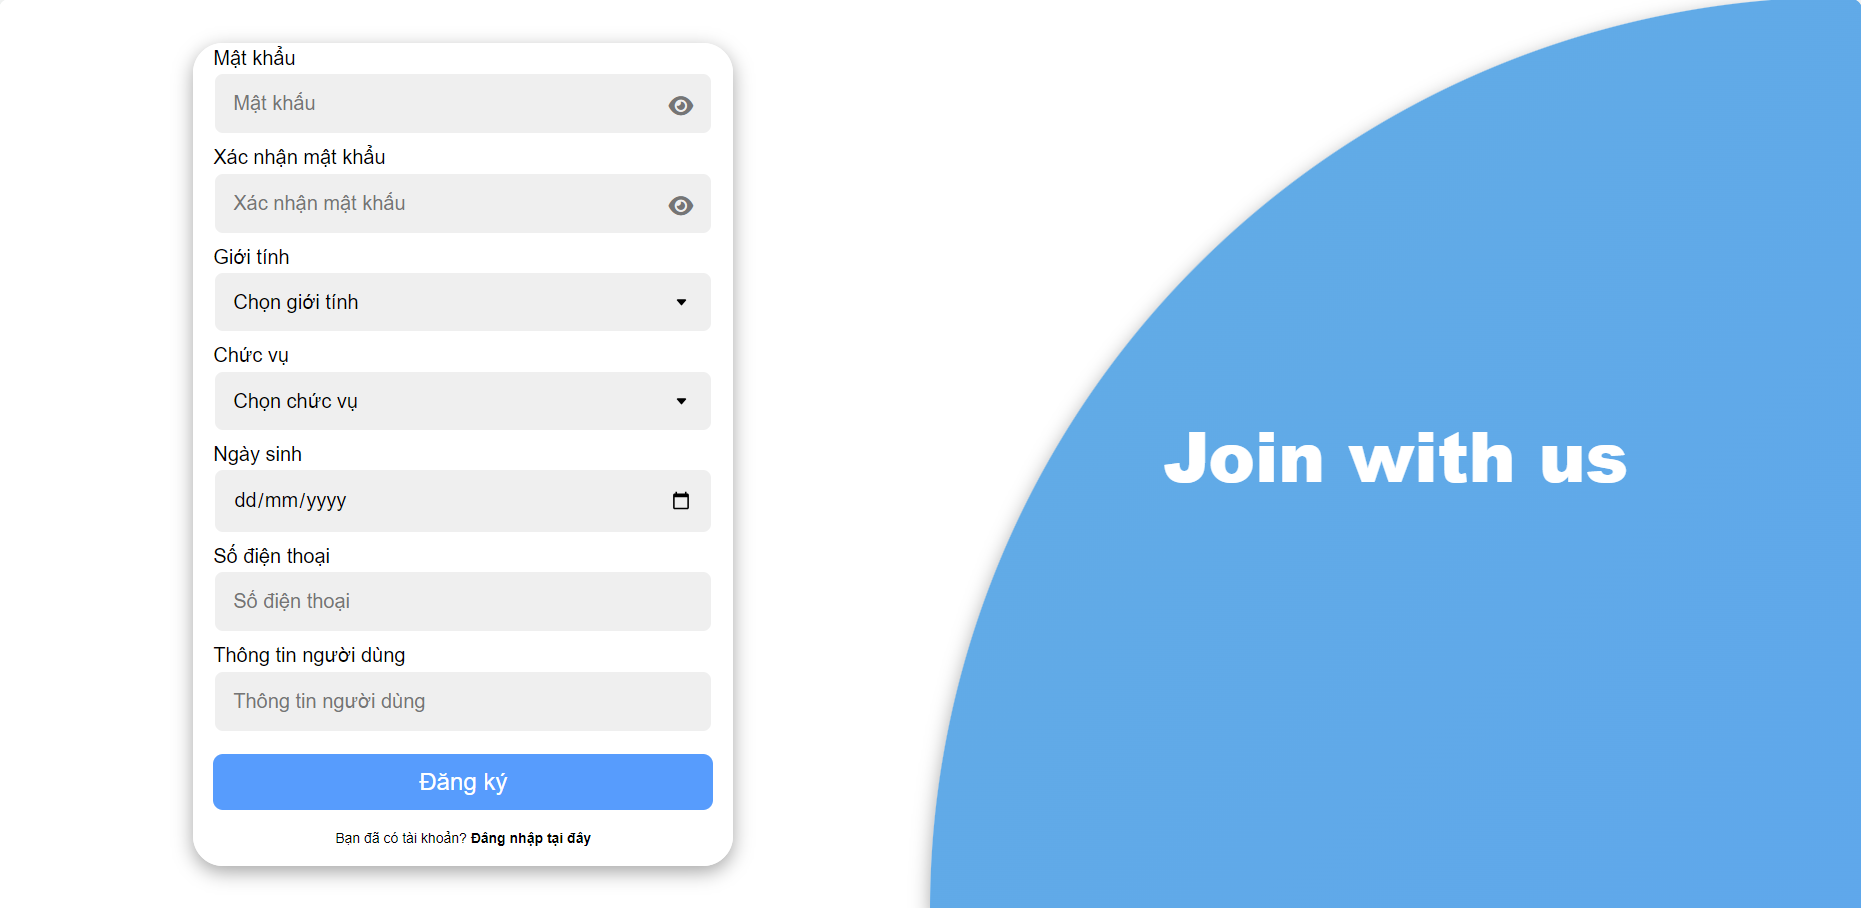
\includegraphics[scale=0.4]{Images/server/webUI/register_2.png}
  \caption[Giao diện trang đăng ký tài khoản]{\bfseries \fontsize{12pt}{0pt}\selectfont Giao diện trang đăng ký tài khoản}
  \label{register_2} %đặt tên cho ảnh
\end{figure}

Hình \ref{register_1}, \ref{register_2} mô tả giao diện cho màn hình đăng ký tài khoản, màn hình này sẽ bao
 gồm các thông tin để người dùng đăng ký tài khoản vào hệ thống
 nếu các thông tin là chính xác thì sẽ chuyển hướng đến trang đăng nhập và chờ kết quả phê duyệt qua email, 
 còn nếu sai thông tin thì sẽ có popup thông báo sai trường thông tin

\begin{figure}[H]
  \centering
  \includegraphics[scale=0.4]{Images/server/webUI/login.png}
  \caption[Giao diện trang đăng nhập]{\bfseries \fontsize{12pt}{0pt}\selectfont Giao diện trang đăng nhập}
  \label{login} %đặt tên cho ảnh
\end{figure}

Hình \ref{login} mô tả giao diện cho màn hình đăng nhập, màn hình này sẽ bao
 gồm hai trường thông tin là Tên đăng nhập và Mật khẩu để người dùng đăng nhập vào trang quản trị.
 Nếu các thông tin là chính xác với CSDL thì màn hình sẽ chuyển hướng đến trang dashboard 
 quản lý, còn nếu sai thông tin thì sẽ có popup thông báo lỗi cụ thể.

 \begin{figure}[H]
  \centering
  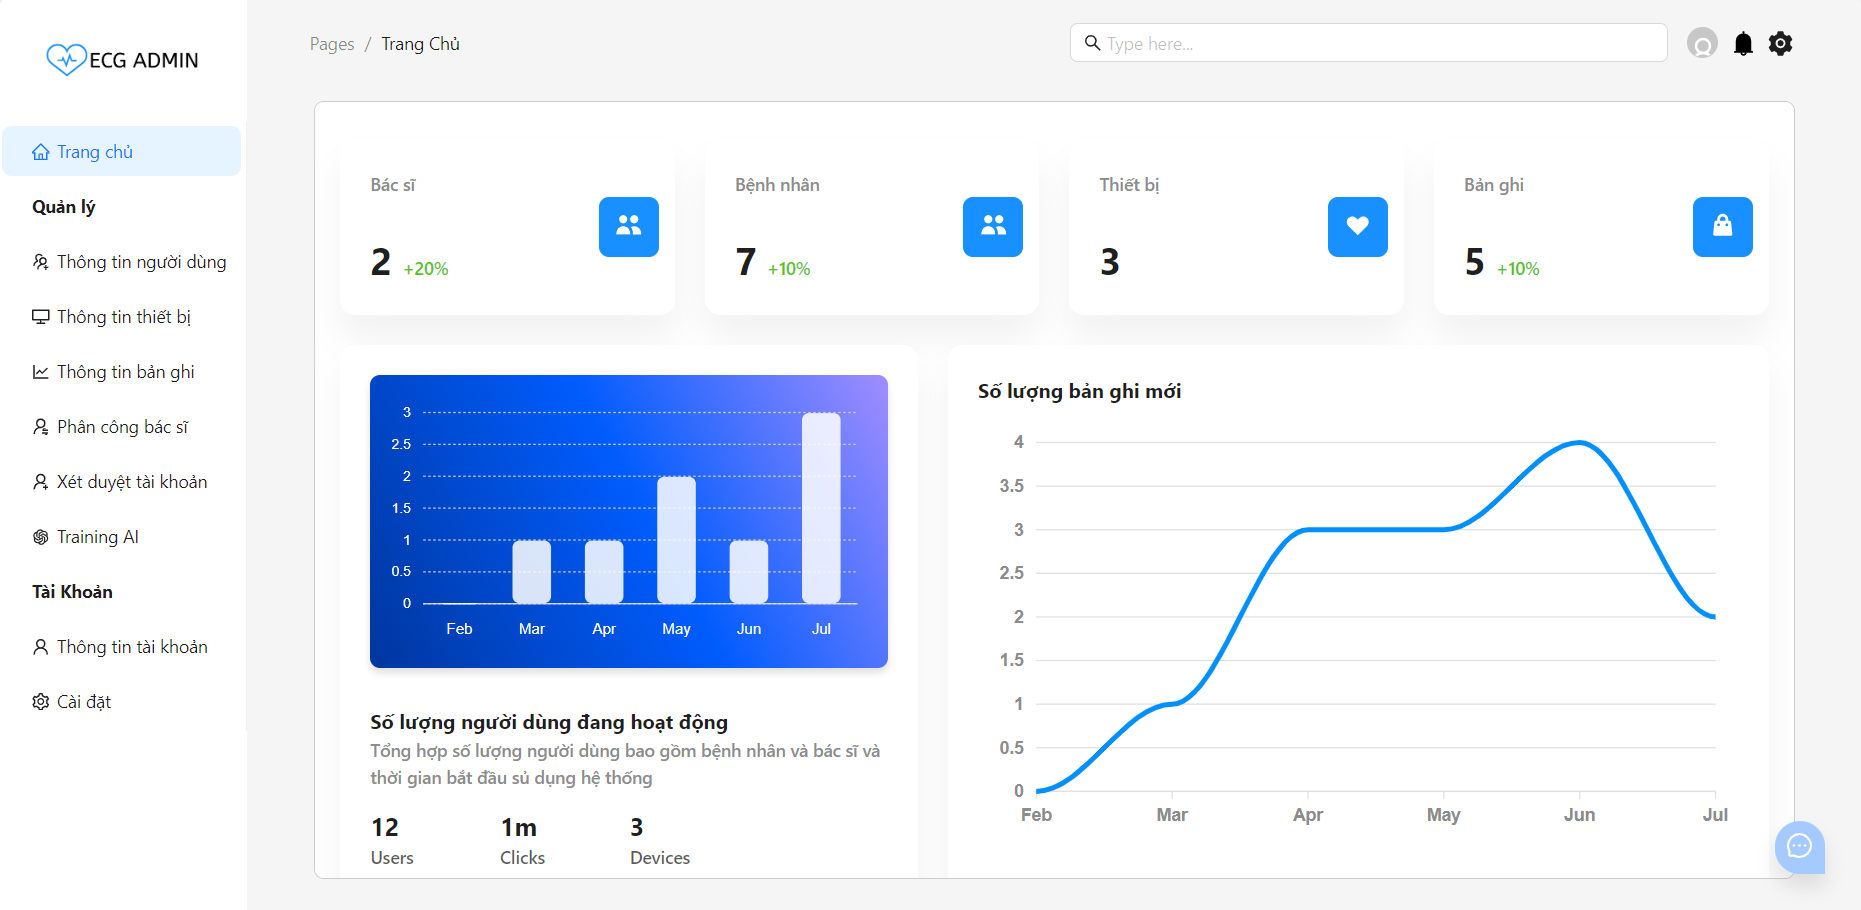
\includegraphics[scale=0.4]{Images/server/webUI/dashboard_admin.png}
  \caption[Giao diện trang dashboard dành cho quản trị viên sau khi đăng nhập thành công]{\bfseries \fontsize{12pt}{0pt}\selectfont Giao diện trang dashboard dành cho admin sau khi đăng nhập thành công}
  \label{dashboard_admin} %đặt tên cho ảnh
\end{figure}

\begin{figure}[H]
  \centering
  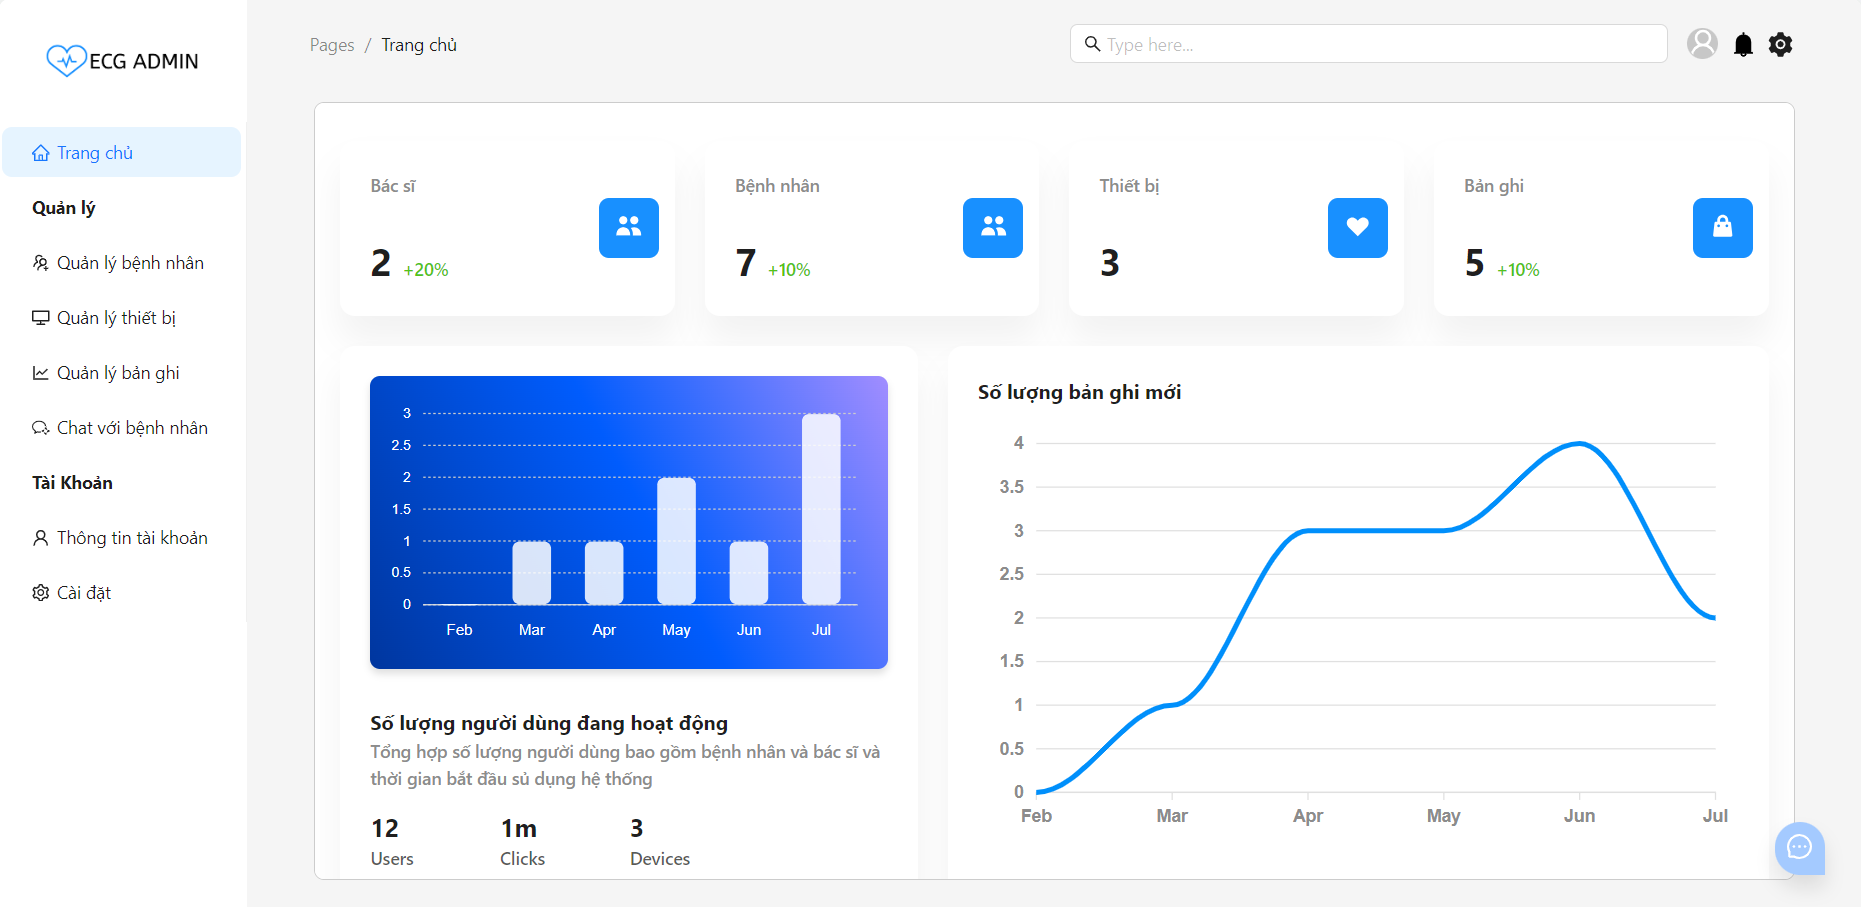
\includegraphics[scale=0.4]{Images/server/webUI/dashboard_doctor.png}
  \caption[Giao diện trang dashboard dành cho bác sĩ sau khi đăng nhập thành công]{\bfseries \fontsize{12pt}{0pt}\selectfont Giao diện trang dashboard dành cho bác sĩ sau khi đăng nhập thành công}
  \label{dashboard_doctor} %đặt tên cho ảnh
\end{figure}

\begin{figure}[H]
  \centering
  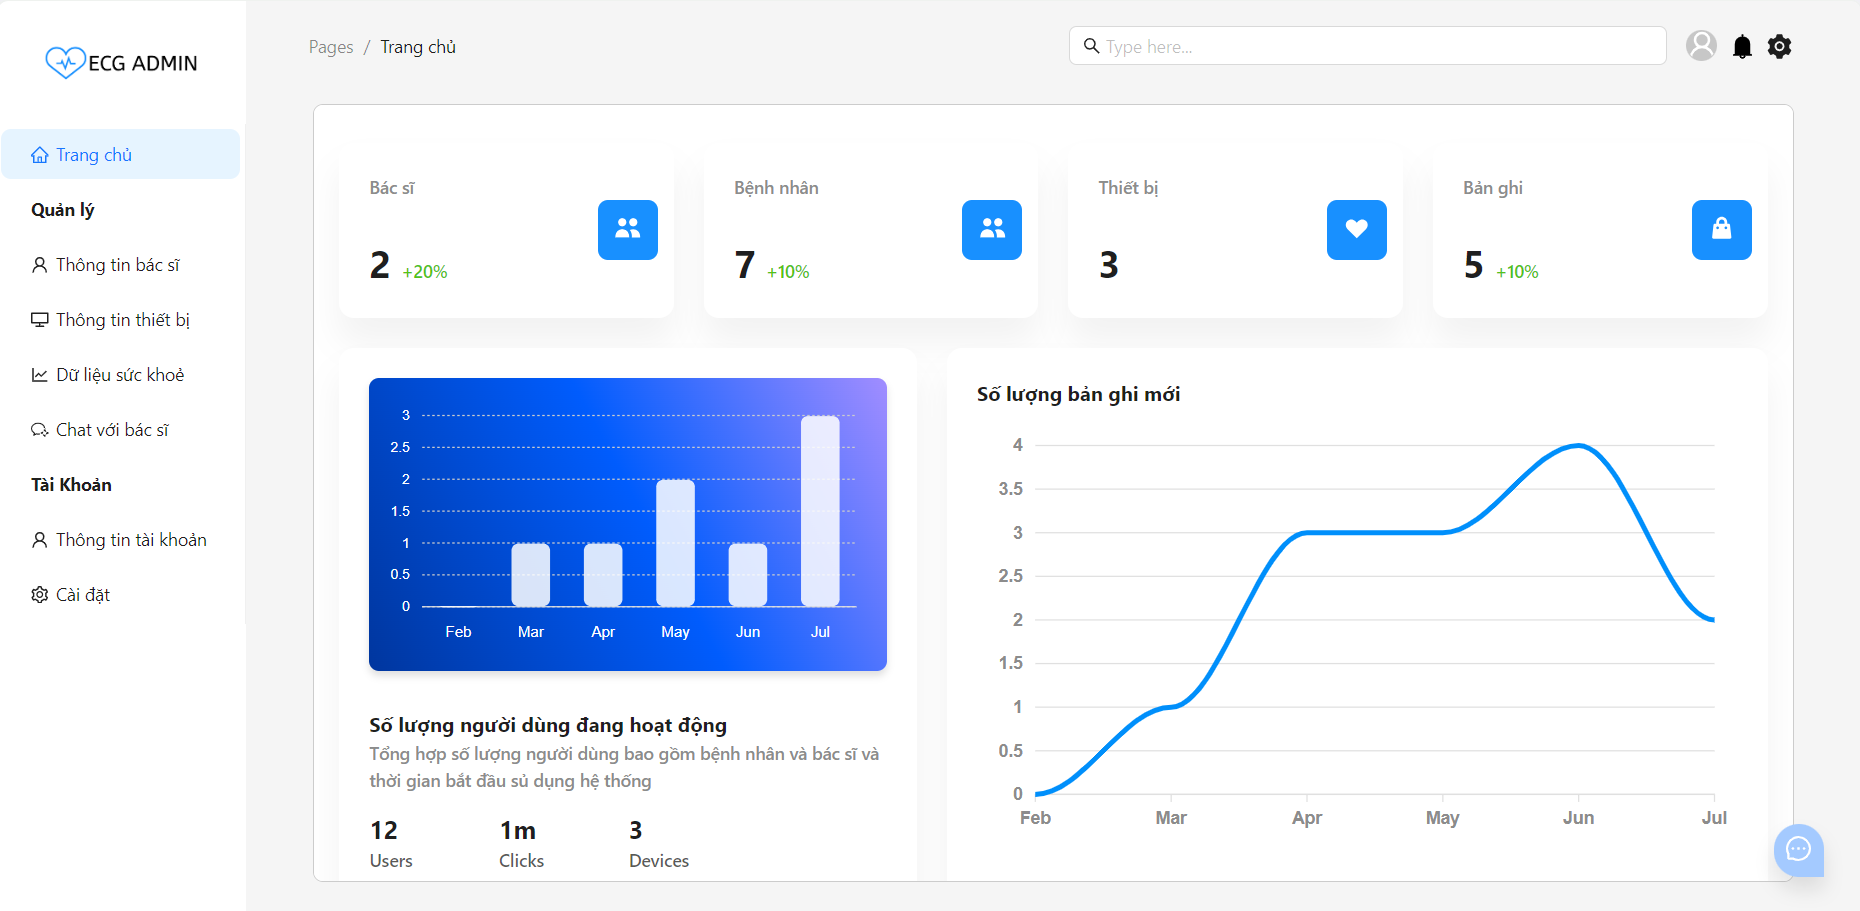
\includegraphics[scale=0.4]{Images/server/webUI/dashboard_patient.png}
  \caption[Giao diện trang dashboard dành cho bệnh nhân sau khi đăng nhập thành công]{\bfseries \fontsize{12pt}{0pt}\selectfont Giao diện trang dashboard dành cho bệnh nhân sau khi đăng nhập thành công}
  \label{dashboard_patient} %đặt tên cho ảnh
\end{figure}

Hình \ref{dashboard_admin}, \ref{dashboard_doctor}, \ref{dashboard_patient} mô tả giao diện cho trang dashboard, trong màn hình này phần bên trái sẽ bao
 gồm thanh điều hướng dẫn đến trang quản lý từng mục khác nhau theo từng loại tài khoản (quản trị viên, bác sĩ, bệnh nhân) và 
 thông tin tài khoản. Còn ở giữa là thông tin tổng số các mục mà hệ thống quản lý (người dùng, thiết bị, bản ghi)
 cùng với đó là biểu đồ thống kê số lượng người dùng và bản ghi mới theo tháng.

\begin{figure}[H]
  \centering
  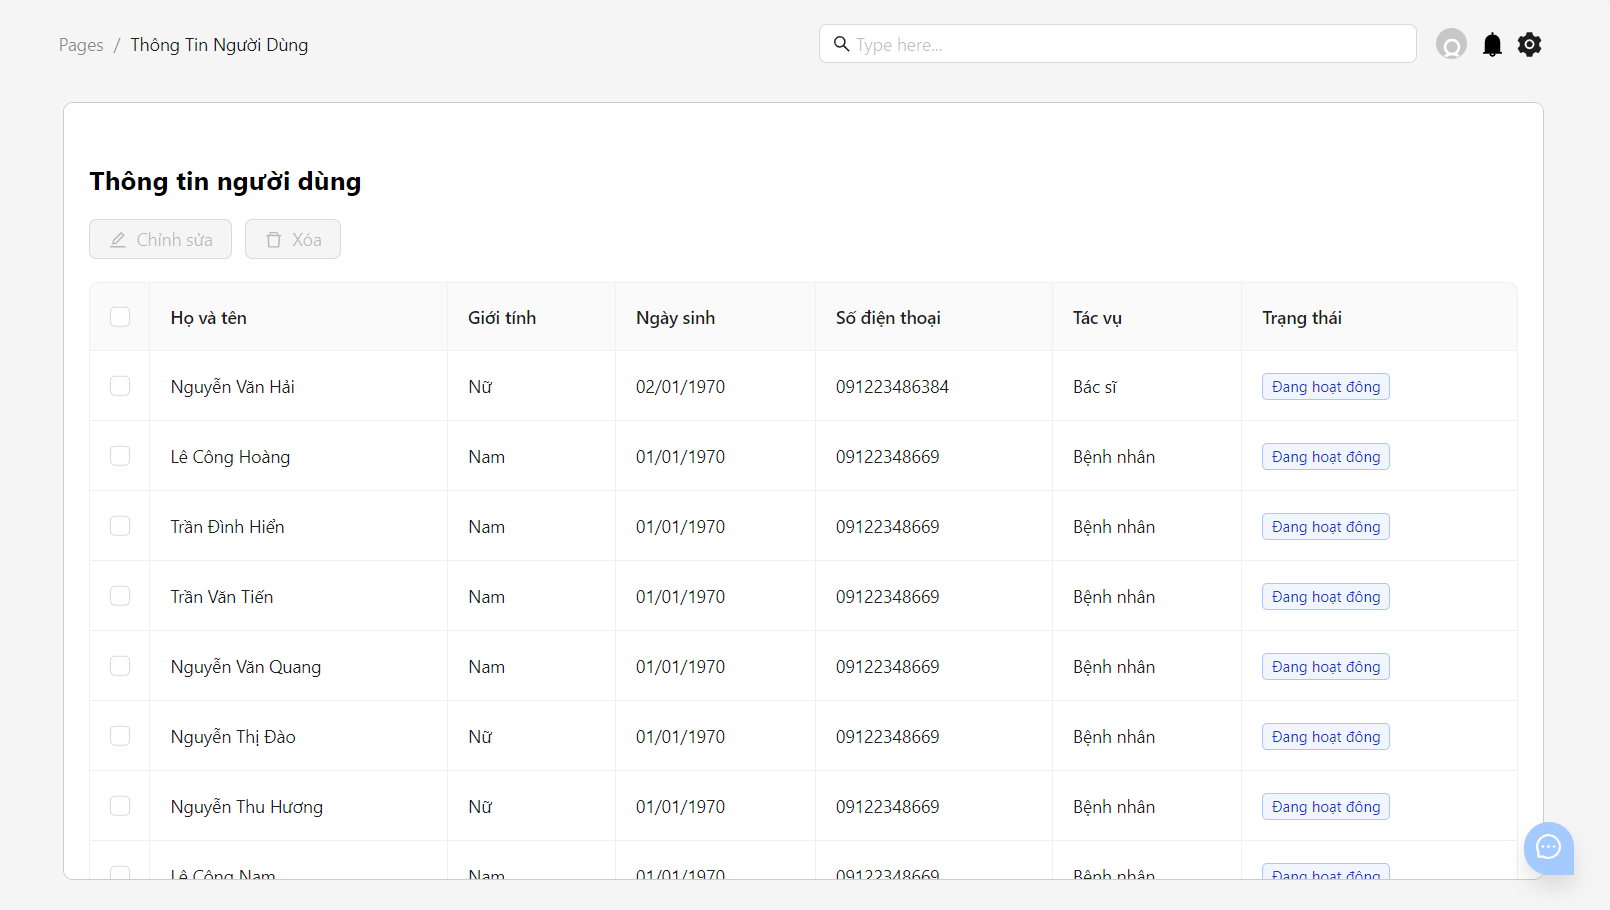
\includegraphics[scale=0.5]{Images/server/webUI/userTable.png}
  \caption[Giao diện trang quản lý người dùng]{\bfseries \fontsize{12pt}{0pt}\selectfont Giao diện trang quản lý người dùng}
  \label{userTable} %đặt tên cho ảnh
\end{figure}

Hình \ref{userTable} mô tả giao diện cho trang quản lý người dùng, trang này sẽ hiển thị danh sách
thông tin của các người dùng đang có trên hệ thống. Khi chọn vào từng người dùng, tương ứng sẽ có các 
lựa chọn để xem chi tiết thông tin người dùng, cập nhật thông tin hay xóa nhiều người dùng cùng lúc.

\begin{figure}[H]
  \centering
  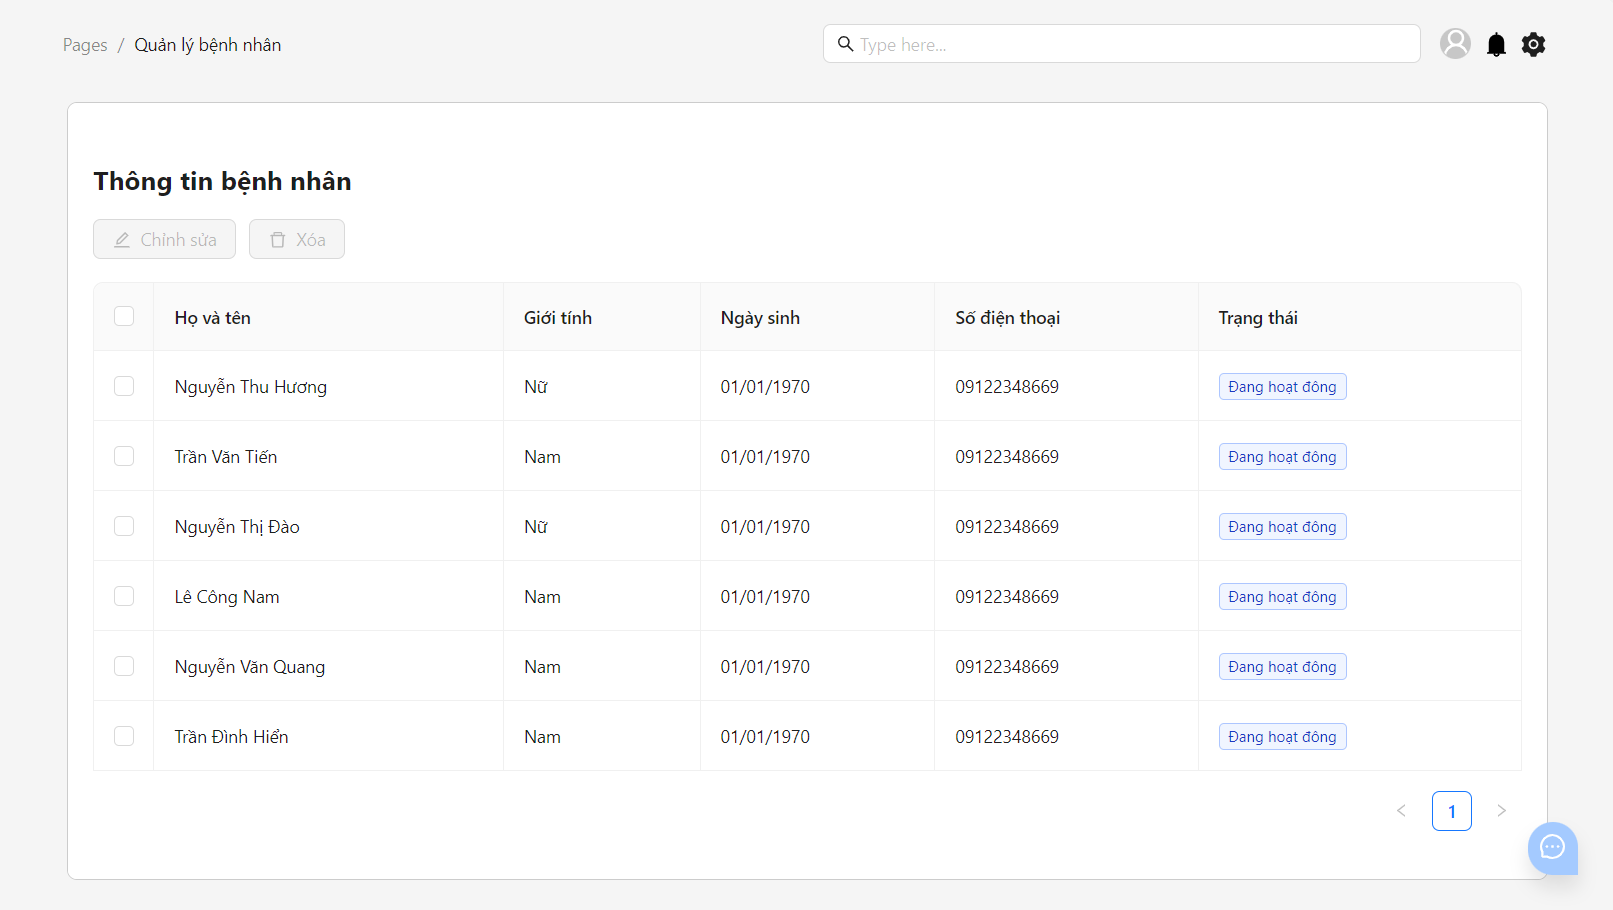
\includegraphics[scale=0.5]{Images/server/webUI/patientTable.png}
  \caption[Giao diện trang quản lý bệnh nhân]{\bfseries \fontsize{12pt}{0pt}\selectfont Giao diện trang quản lý bệnh nhân}
  \label{patientTable} %đặt tên cho ảnh
\end{figure}

Hình \ref{patientTable} mô tả giao diện cho trang quản lý bệnh nhân, trang này có giao diện tương tự với trang 
quản lý người dùng ở hình \ref{userTable} nhưng thông tin ở đây sẽ dành cho bác sĩ, và trang này chỉ có chức năng xem thông tin bệnh nhân.

\begin{figure}[H]
  \centering
  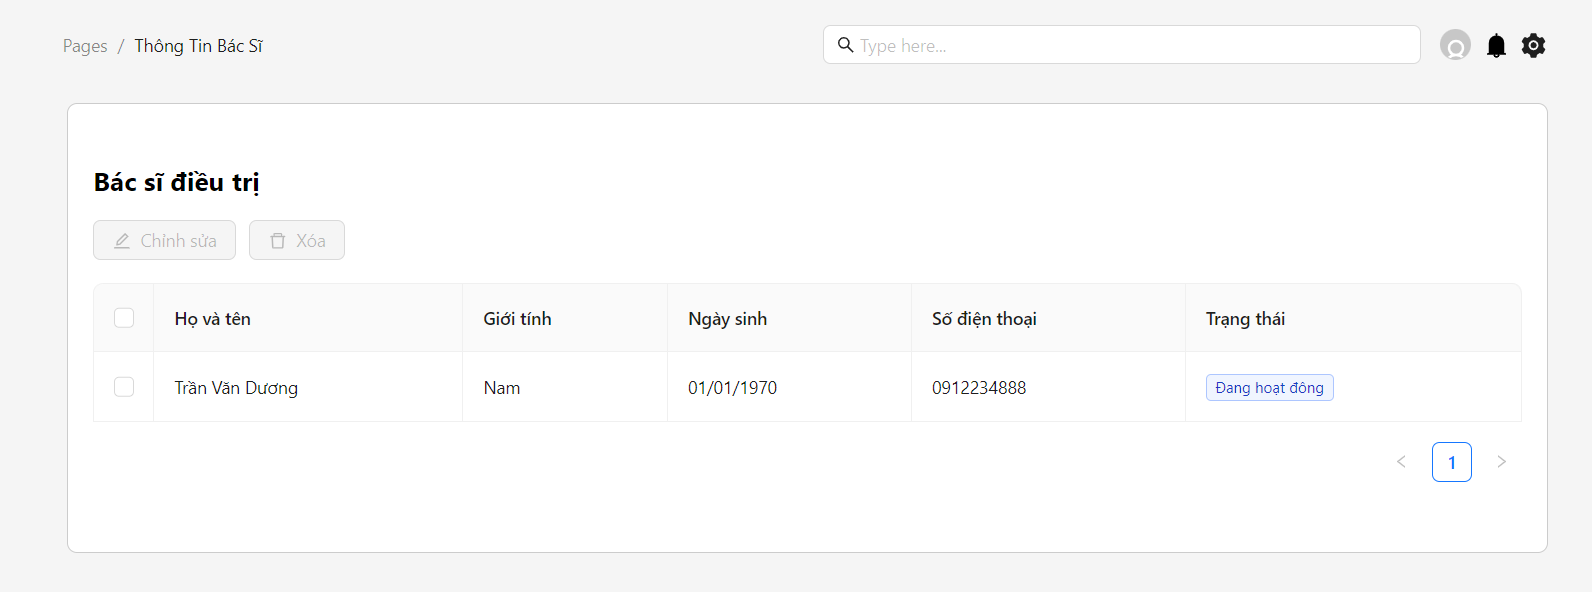
\includegraphics[scale=0.5]{Images/server/webUI/manageDoctor.png}
  \caption[Giao diện trang danh sách bác sĩ phụ trách]{\bfseries \fontsize{12pt}{0pt}\selectfont Giao diện trang danh sách bác sĩ phụ trách}
  \label{doctorTable} %đặt tên cho ảnh
\end{figure}

Hình \ref{doctorTable} mô tả giao diện cho trang danh sách bác sĩ phụ trách, trang này có giao diện tương tự với trang 
quản lý người dùng ở hình \ref{userTable} nhưng thông tin ở đây sẽ dành cho bệnh nhân, và trang này chỉ có chức năng xem thông tin bác sĩ.

\begin{figure}[H]
  \centering
  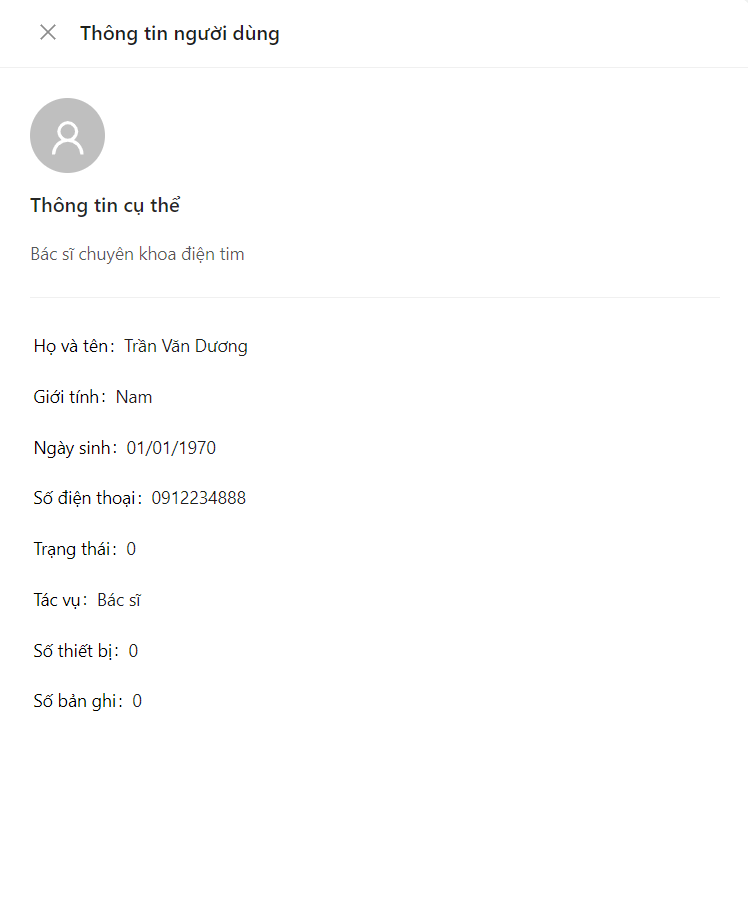
\includegraphics[scale=0.6]{Images/server/webUI/userInfo.png}
  \caption[Giao diện màn thông tin chi tiết người dùng]{\bfseries \fontsize{12pt}{0pt}\selectfont Giao diện màn thông tin chi tiết người dùng}
  \label{userInfo} %đặt tên cho ảnh
\end{figure}

Hình \ref{userInfo} mô tả giao diện cho màn thông tin chi tiết người dùng, màn này sẽ hiển thị thông tin
chi tiết của người dùng trong danh sách.

\begin{figure}[H]
  \centering
  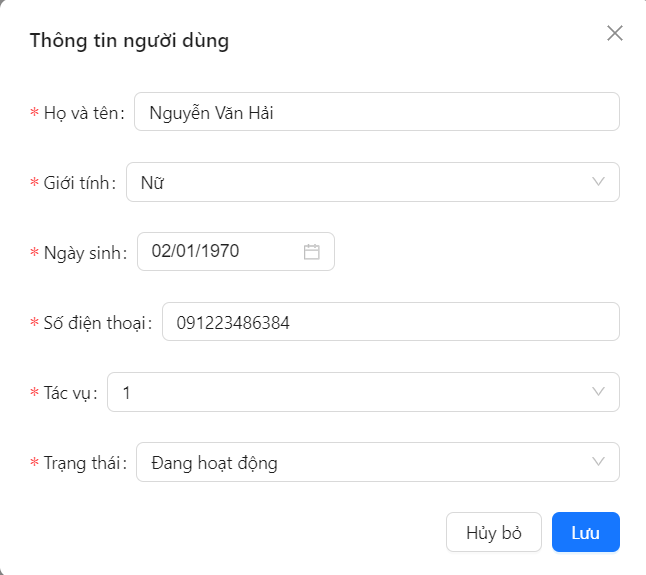
\includegraphics[scale=0.7]{Images/server/webUI/updateUser.png}
  \caption[Giao diện màn cập nhật thông tin người dùng]{\bfseries \fontsize{12pt}{0pt}\selectfont Giao diện màn cập nhật thông tin người dùng}
  \label{editUser} %đặt tên cho ảnh
\end{figure}

Hình \ref{editUser} mô tả giao diện cho màn cập nhật thông tin người dùng. Màn này sẽ hiển thị form chỉnh sửa bao gồm 
tên, giới tính, ngày sinh, số điện thoại, tác vụ, trạng thái. Trên các trường sẽ hiện thông tin người dùng mà admin đã chọn. 
Admin sẽ chỉnh sửa thông tin, sau đó nhấn nút Lưu để lưu dữ liệu.

\begin{figure}[H]
  \centering
  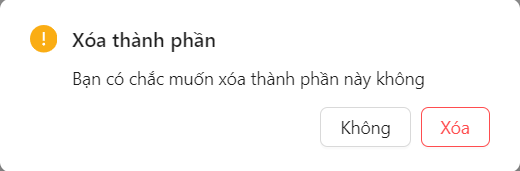
\includegraphics[scale=0.7]{Images/server/webUI/delete.png}
  \caption[Giao diện màn xóa thông tin trong trang quản lý]{\bfseries \fontsize{12pt}{0pt}\selectfont Giao diện màn xóa thông tin trong trang quản lý}
  \label{delete} %đặt tên cho ảnh
\end{figure}

Hình \ref{delete} mô tả giao diện cho màn xóa thông tin trong trang quản lý. Màn này sẽ hiện lên thông tin xác nhận người dùng có muốn 
xóa trường thông tin ấy không. Nếu người dùng muốn xóa sẽ nhấn nút Xóa, còn nếu không sẽ nhấn nút Hủy bỏ.

\begin{figure}[H]
  \centering
  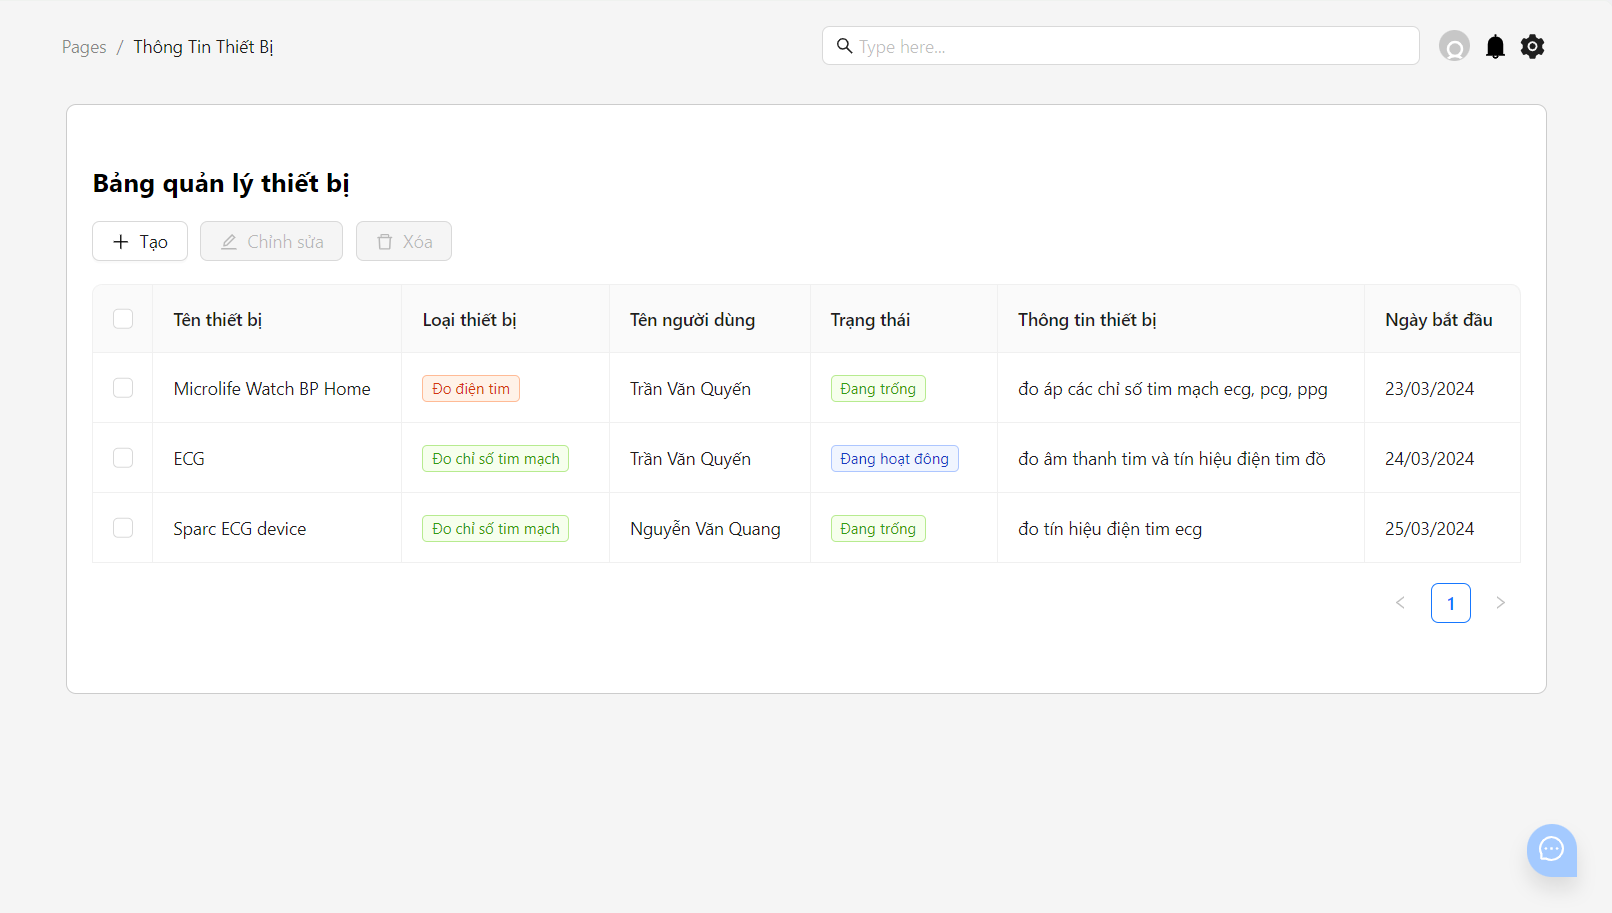
\includegraphics[scale=0.5]{Images/server/webUI/deviceTable.png}
  \caption[Giao diện trang quản lý thiết bị]{\bfseries \fontsize{12pt}{0pt}\selectfont Giao diện trang quản lý thiết bị}
  \label{deviceTable} %đặt tên cho ảnh
\end{figure}

Hình \ref{deviceTable} mô tả giao diện cho trang quản lý thiết bị, trang này sẽ có giao diện tương tự trang quản lý người dùng. 
Tương tự khi tích vào mỗi thiết bị tương ứng sẽ có các lựa chọn xem chi tiết thông tin, sửa thông tin thiết bị.
Bên cạnh đó sẽ có thêm nút bấm để tạo mới thông tin thiết bị.
\begin{figure}[H]
  \centering
  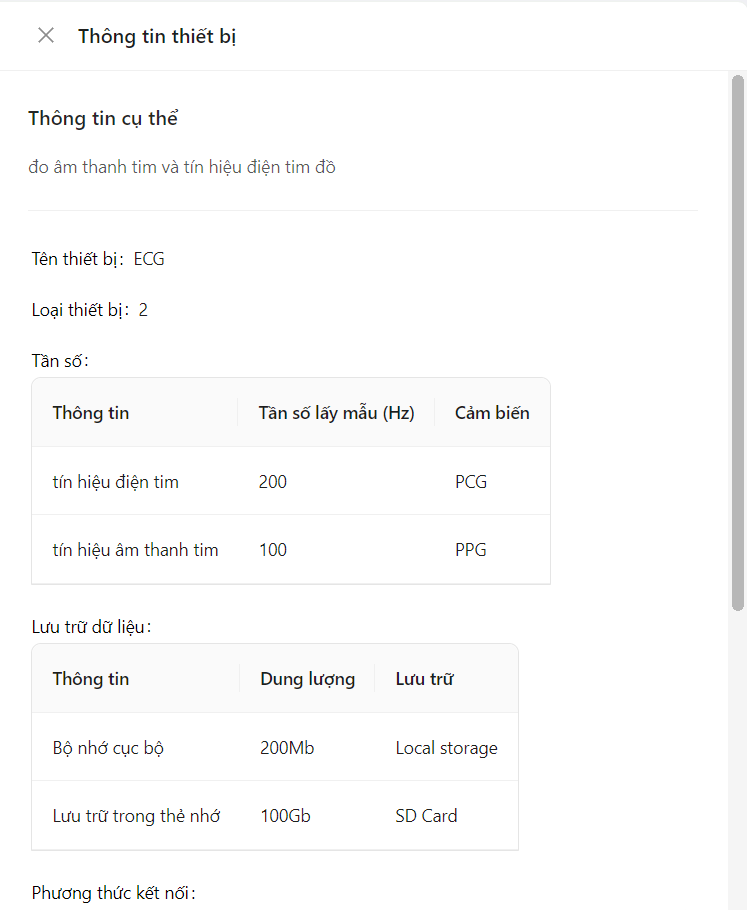
\includegraphics[scale=0.7]{Images/server/webUI/deviceInfo_1.png}
  \caption[Giao diện màn thông tin chi tiết thiết bị]{\bfseries \fontsize{12pt}{0pt}\selectfont Giao diện màn thông tin chi tiết thiết bị}
  \label{deviceInfo} %đặt tên cho ảnh
\end{figure}

Hình \ref{deviceInfo} mô tả giao diện cho màn thông tin chi tiết thiết bị, màn này sẽ hiển thị thông tin
chi tiết của thiết bị khi quản trị viên chọn vào một thiết bị trong danh sách.

\begin{figure}[H]
  \centering
  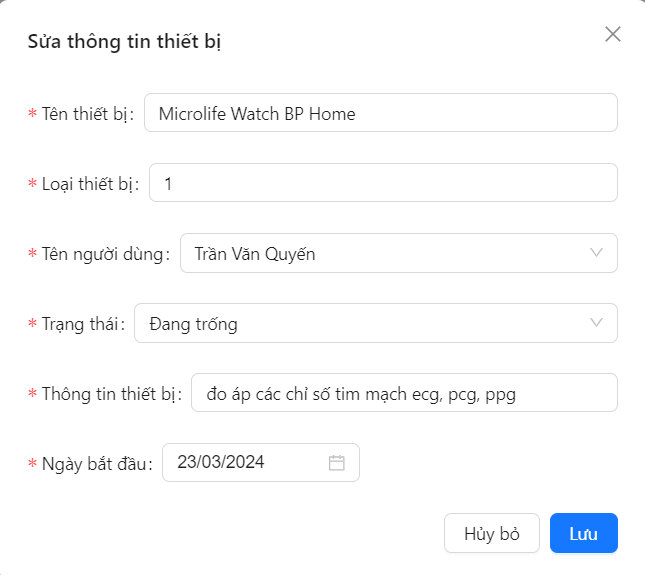
\includegraphics[scale=0.7]{Images/server/webUI/editDevice.png}
  \caption[Giao diện màn cập nhật thông tin thiết bị]{\bfseries \fontsize{12pt}{0pt}\selectfont Giao diện màn cập nhật thông tin thiết bị}
  \label{editDevice} %đặt tên cho ảnh
\end{figure}

Hình \ref{editDevice} mô tả giao diện cho màn cập nhật thông tin thiết bị. Màn này sẽ có các trường thông tin bao gồm 
tên thiết bị, loại thiết bị, tên người dùng, trạng thái, thông tin, ngày bắt đầu. Trên các trường sẽ hiện thông tin thiết bị mà quản trị viên đã chọn. 
Admin sẽ chỉnh sửa thông tin, sau đó nhấn nút Lưu để lưu dữ liệu.

\begin{figure}[H]
  \centering
  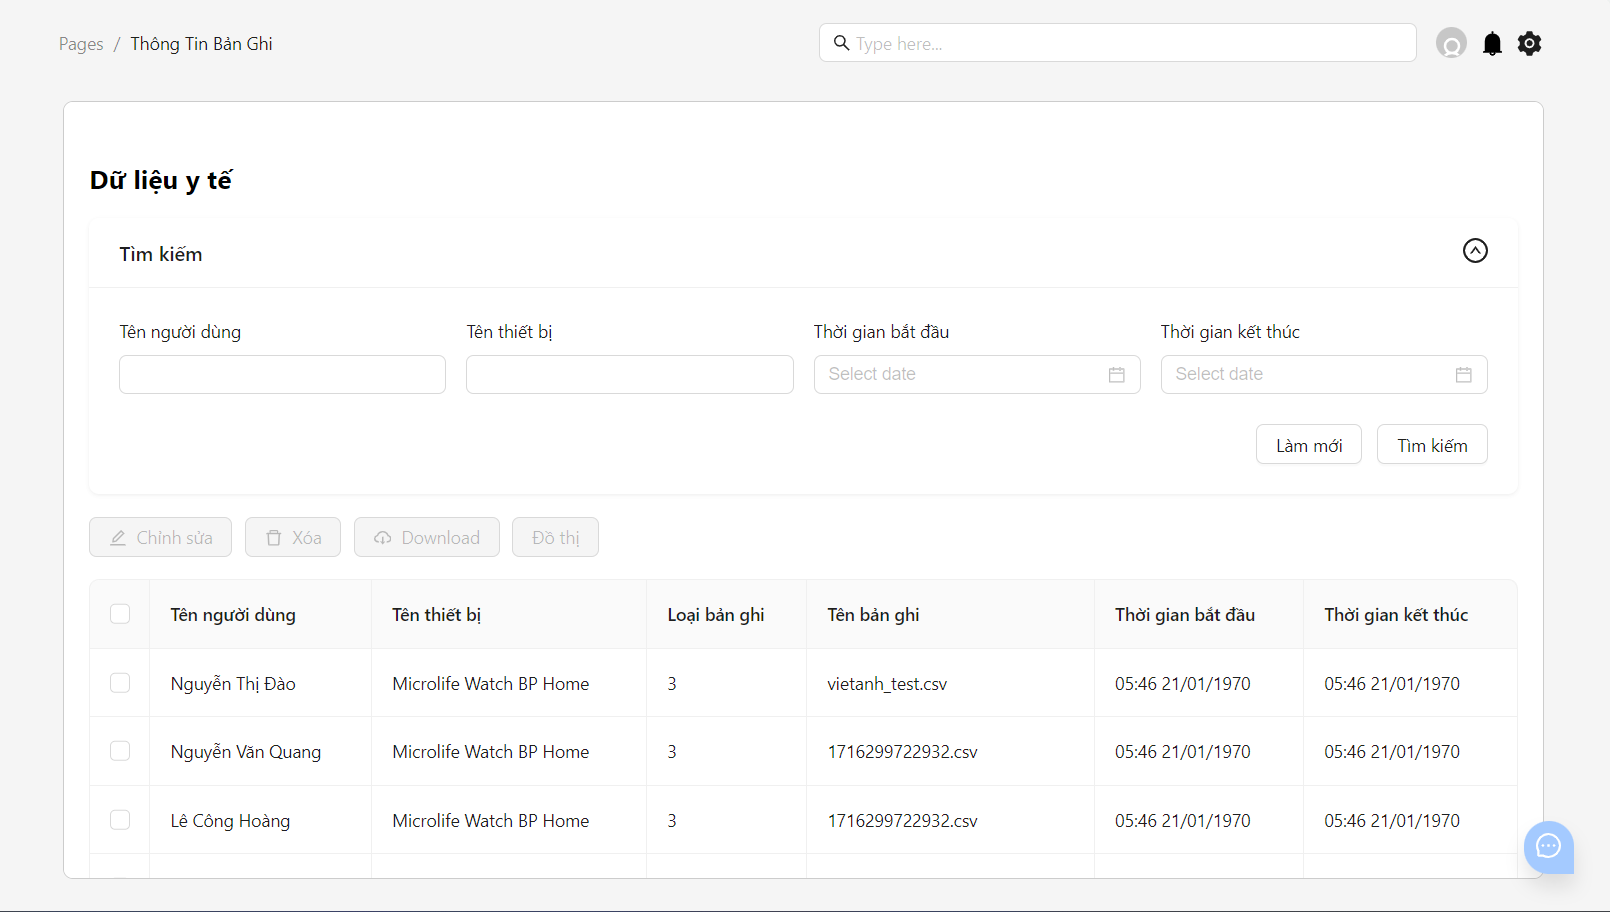
\includegraphics[scale=0.5]{Images/server/webUI/recordTable.png}
  \caption[Giao diện trang quản lý phiên đo]{\bfseries \fontsize{12pt}{0pt}\selectfont Giao diện trang quản lý phiên đo}
  \label{recordTable} %đặt tên cho ảnh
\end{figure}

Hình \ref{recordTable} mô tả giao diện cho trang quản lý phiên đo, trang này sẽ hiển thị danh sách
thông tin của các phiên đo trên hệ thống, bên cạnh đó khi tích vào mỗi phiên đo tương ứng sẽ 
có các lựa chọn để cập nhật thông tin, xóa thông tin, tải bản ghi cũng như xem đồ thị phiên đo. 

\begin{figure}[H]
  \centering
  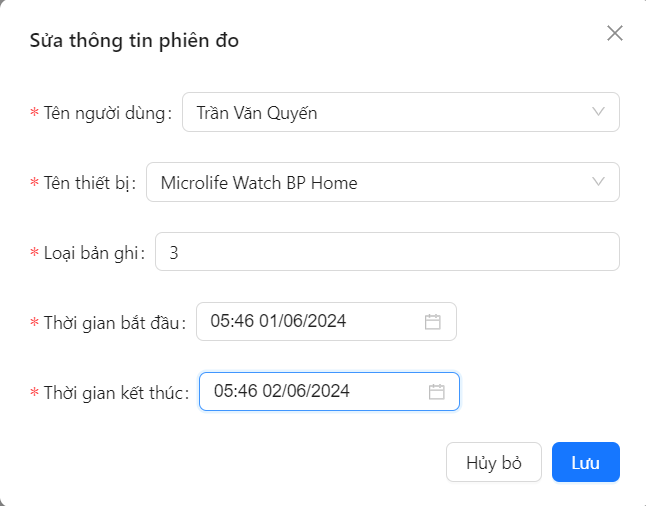
\includegraphics[scale=0.7]{Images/server/webUI/editRecord.png}
  \caption[Giao diện màn cập nhật thông tin phiên đo]{\bfseries \fontsize{12pt}{0pt}\selectfont Giao diện màn cập nhật thông tin phiên đo}
  \label{editRecord} %đặt tên cho ảnh
\end{figure}

Hình \ref{editRecord} mô tả giao diện cho màn cập nhật thông tin thiết bị. Màn này sẽ có các trường thông tin bao gồm 
tên người dùng, tên thiết bị, loại bản ghi, thời gian bắt đầu, thời gian kết thúc. Trên các trường sẽ hiện thông tin phiên đo mà quản trị viên đã chọn. 
Admin sẽ chỉnh sửa thông tin, sau đó nhấn nút Lưu để lưu dữ liệu.

\begin{figure}[H]
  \centering
  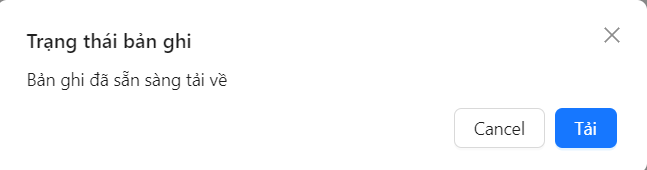
\includegraphics[scale=0.7]{Images/server/webUI/downloadRecord.png}
  \caption[Giao diện màn tải bản ghi dữ liệu phiên đo]{\bfseries \fontsize{12pt}{0pt}\selectfont Giao diện màn tải bản ghi dữ liệu phiên đo}
  \label{downloadRecord} %đặt tên cho ảnh
\end{figure}

Hình \ref{downloadRecord} mô tả giao diện cho màn tải bản ghi dữ liệu phiên đo. Màn này sẽ hiện lên thông tin xác nhận người dùng có muốn 
tải bản ghi dữ liệu phiên đo không cũng như trạng thái tải. Nếu người dùng muốn tải bản ghi sẽ nhấn nút Tải, còn nếu không sẽ nhấn nút Hủy bỏ.

\begin{figure}[H]
  \centering
  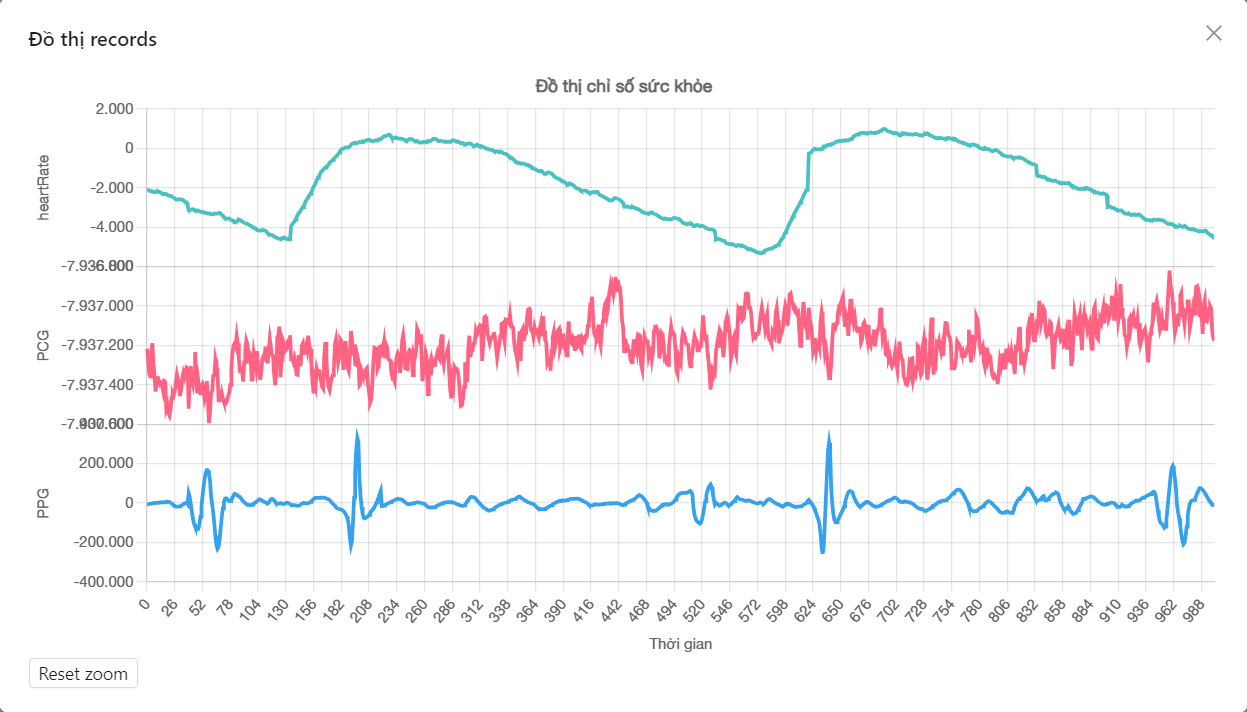
\includegraphics[scale=0.6]{Images/server/webUI/chart.png}
  \caption[Giao diện màn biểu đồ dữ liệu phiên đo]{\bfseries \fontsize{12pt}{0pt}\selectfont Giao diện màn biểu đồ dữ liệu phiên đo}
  \label{recordChart} %đặt tên cho ảnh
\end{figure}

Hình \ref{recordChart} mô tả giao diện cho màn biểu đồ dữ liệu phiên đo. Màn này sẽ hiện lên thông tin dữ liệu phiên đo theo biểu đồ đường, người dùng 
có thể phóng to thu nhỏ. Nếu có nhiều hơn một dữ liệu đo, thể hiện qua màu sắc các đường và trục tung sẽ hiển thị tên kênh đo dữ liệu giúp người dùng dễ dàng theo dõi.

\begin{figure}[H]
  \centering
  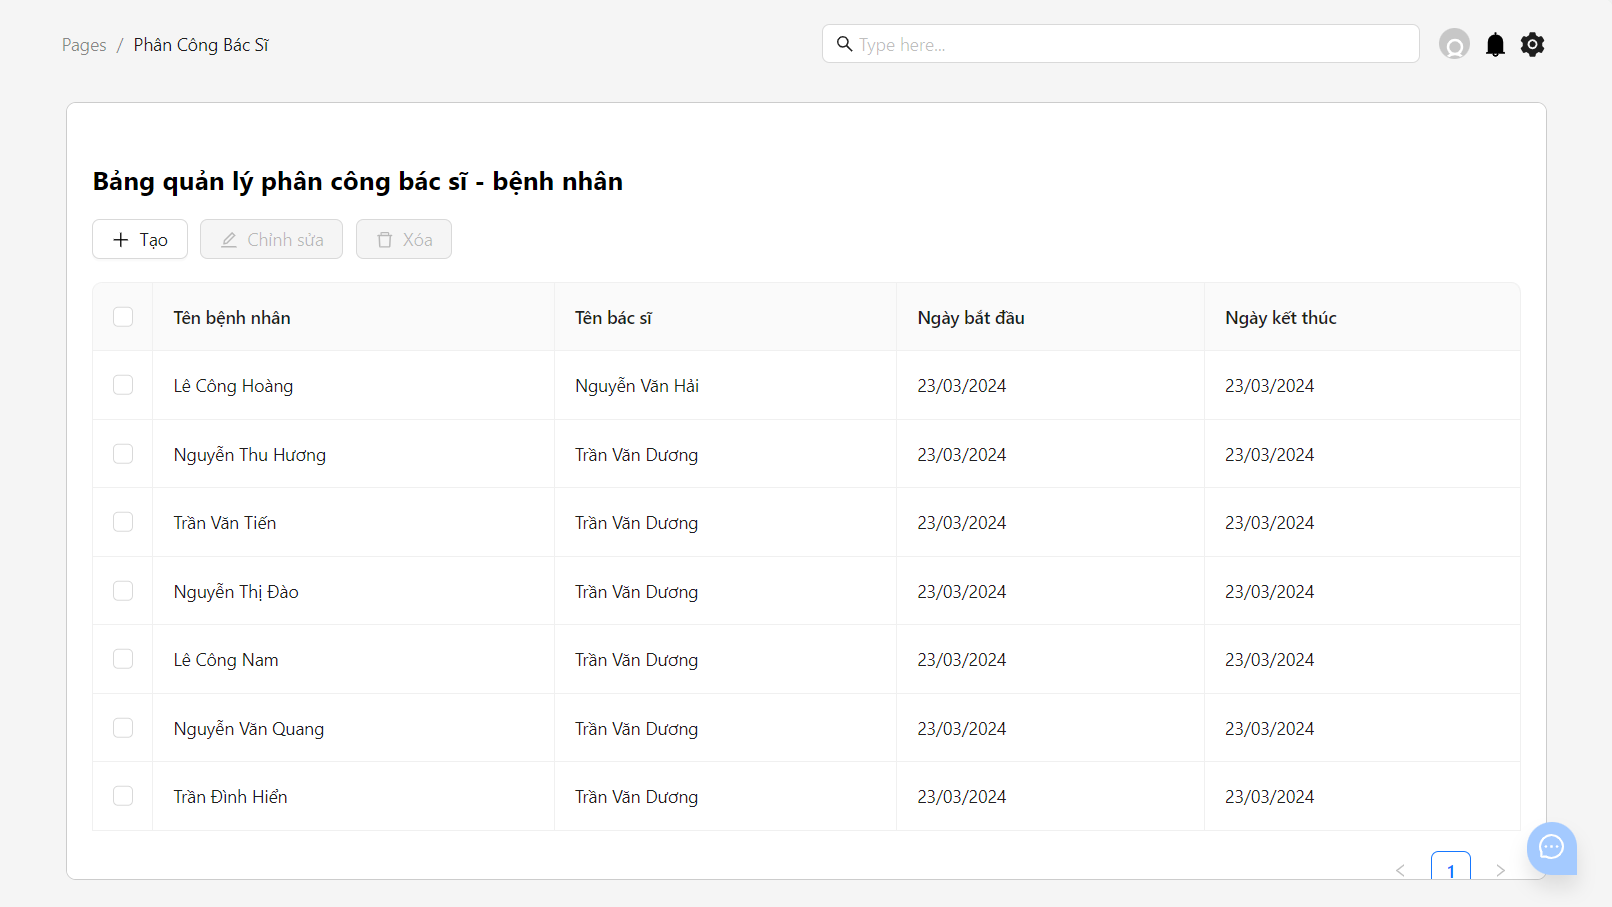
\includegraphics[scale=0.5]{Images/server/webUI/pdaTable.png}
  \caption[Giao diện trang quản lý phân công bác sĩ - bệnh nhân]{\bfseries \fontsize{12pt}{0pt}\selectfont Giao diện trang quản lý phân công bác sĩ - bệnh nhân}
  \label{pdaTable} %đặt tên cho ảnh
\end{figure}

Hình \ref{pdaTable} mô tả giao diện cho trang quản lý phân công bác sĩ - bệnh nhân, trang này sẽ có giao diện hiển thị danh sách phân công tương tự với các trang quản lý khác . 
Khi chọn vào mỗi phân công tương ứng sẽ có các lựa chọn để cập nhật phân công, xóa nhiều phân công cùng một lúc, và sẽ có nút tạo phân công mới. 

\begin{figure}[H]
  \centering
  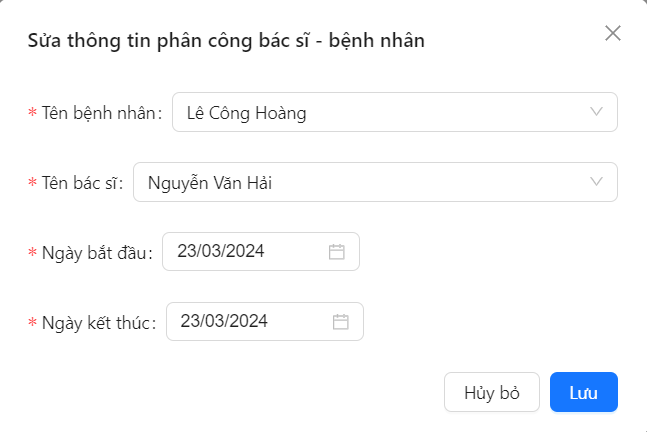
\includegraphics[scale=0.7]{Images/server/webUI/editPDA.png}
  \caption[Giao diện màn cập nhật thông tin phân công bác sĩ - bệnh nhân]{\bfseries \fontsize{12pt}{0pt}\selectfont Giao diện màn cập nhật thông tin phân công bác sĩ - bệnh nhân}
  \label{editPDA} %đặt tên cho ảnh
\end{figure}

Hình \ref{editPDA} mô tả giao diện cho màn cập nhật thông tin phân công bác sĩ - bệnh nhân. Màn này sẽ có các trường thông tin bao gồm 
tên bác sĩ, tên bệnh nhân, ngày bắt đầu, ngày kết thúc. Trên các trường sẽ hiện thông tin phân công mà quản trị viên đã chọn. 
Admin sẽ chỉnh sửa thông tin, sau đó nhấn nút Lưu để lưu dữ liệu.

\begin{figure}[H]
  \centering
  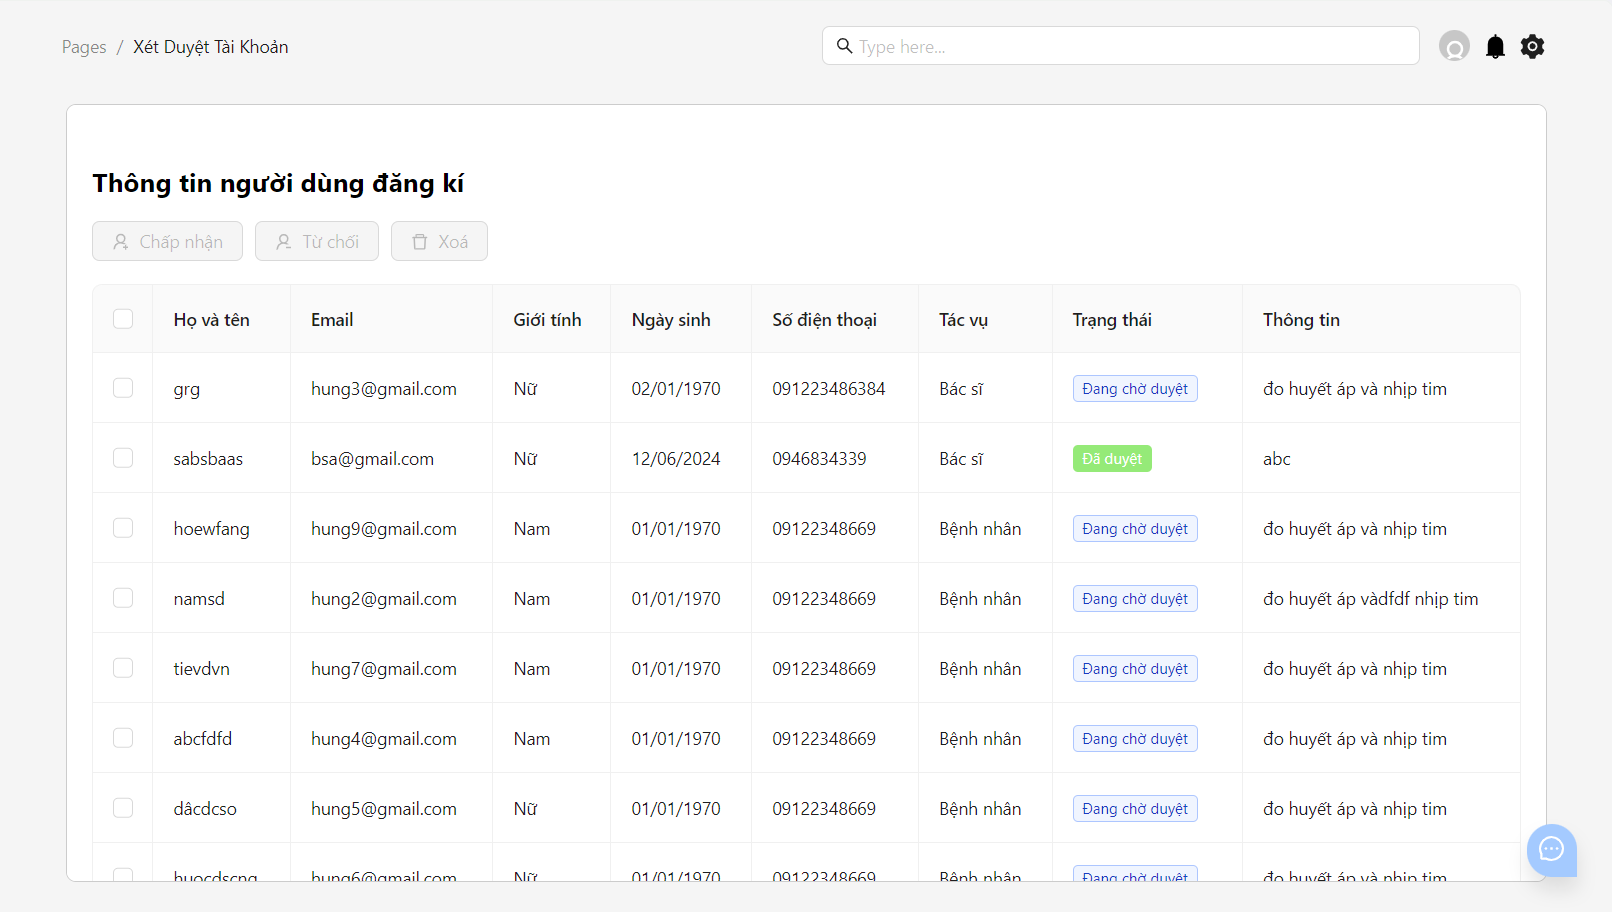
\includegraphics[scale=0.5]{Images/server/webUI/registerTable.png}
  \caption[Giao diện trang quản lý phê duyệt tài khoản]{\bfseries \fontsize{12pt}{0pt}\selectfont Giao diện trang xét duyệt tài khoản đăng ký}
  \label{registerTable} %đặt tên cho ảnh
\end{figure}

Hình \ref{registerTable} mô tả giao diện cho trang quản lý phê duyệt tài khoản đăng ký, trang này sẽ hiển thị danh sách
thông tin của tài khoản đang chờ duyệt trên hệ thống, bên cạnh đó khi tích vào mỗi tài khoản tương ứng sẽ 
có các lựa chọn để phê duyệt, từ chối tài khoản.

\begin{figure}[H]
  \centering
  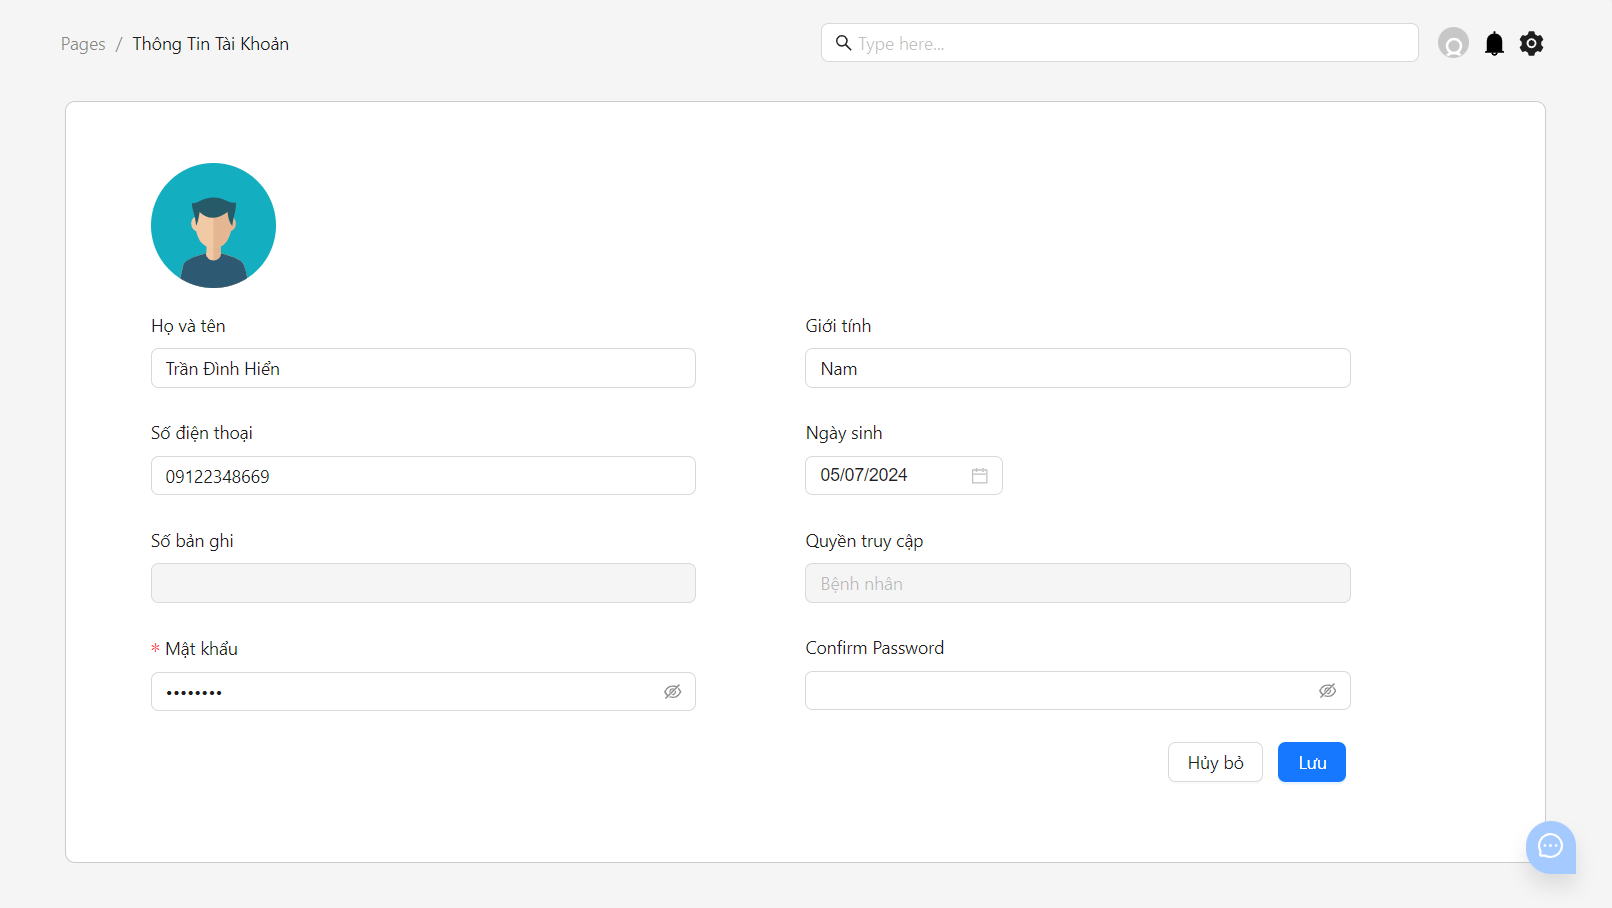
\includegraphics[scale=0.5]{Images/server/webUI/accountInfo.png}
  \caption[Giao diện trang thông tin tài khoản]{\bfseries \fontsize{12pt}{0pt}\selectfont Giao diện màn cập nhật thông tin phân công bác sĩ - bệnh nhân}
  \label{accountInfo} %đặt tên cho ảnh
\end{figure}

Hình \ref{accountInfo} mô tả giao diện cho trang thông tin tài khoản. Trang này sẽ có các trường thông tin bao gồm 
họ và tên, giới tính, số điện thoại, ngày sinh, số bản ghi, quyền truy cập, mật khẩu và xác nhận mật khẩu. Trên các trường sẽ hiện thông tin của tài khoản. 
Người dùng sẽ chỉnh sửa thông tin, sau đó nhấn nút Lưu để lưu dữ liệu.

\begin{figure}[H]
  \centering
  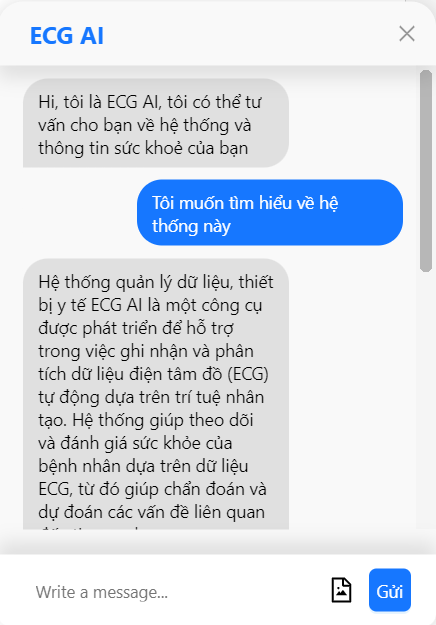
\includegraphics[scale=0.5]{Images/server/webUI/chat_ai.png}
  \caption[Giao diện màn hỏi, nhận tư vấn từ AI]{\bfseries \fontsize{12pt}{0pt}\selectfont Giao diện màn hỏi, nhận tư vấn từ AI}
  \label{chatAI} %đặt tên cho ảnh
\end{figure}

Hình \ref{chatAI} mô tả giao diện cho màn hỏi, nhận tư vấn từ AI. Khi người dùng nhấn vào nút ở góc phải màn hình sẽ hiện lên màn chat với AI. 
Người dùng có thể bắt đầu nhắn tin ở thanh nhắn tin, các tin nhắn sẽ hiển thị theo thứ tự trên xuống. Khi người dùng nhắn một tin, tin nhắn sẽ hiện ở dưới cùng và 
có màu xanh, còn tin nhắn phản hồi từ AI sẽ có nền màu xám. 

\begin{figure}[H]
  \centering
  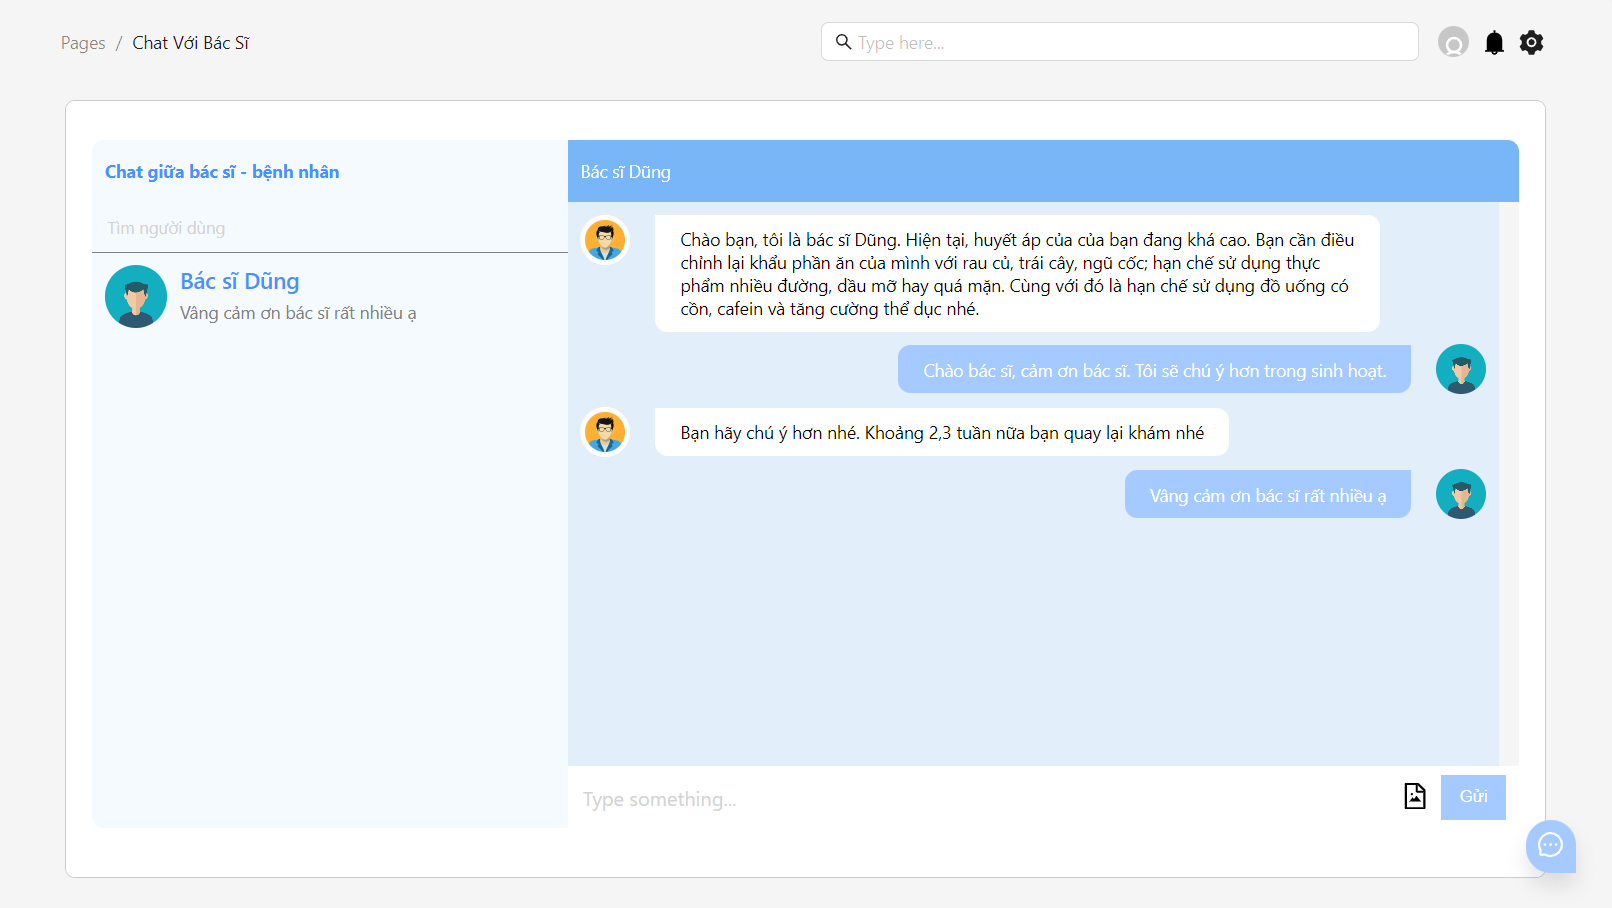
\includegraphics[scale=0.5]{Images/server/webUI/chat.png}
  \caption[Giao diện trang chi tiết hội thoại bệnh nhân, bác sĩ]{\bfseries \fontsize{12pt}{0pt}\selectfont Giao diện trang hỏi, nhận tư vấn từ AI}
  \label{chat} %đặt tên cho ảnh
\end{figure}

Hình \ref{chat} mô tả giao diện cho trang chi tiết hội thoại bệnh nhân, bác sĩ. Ở trong trang này, phía bên trái là danh sách các bệnh nhân, bác sĩ 
bao gồm tên và tin nhắn cuối mà người dùng đã trò chuyện, bên phải là nội dung chi tiết cuộc hội thoại. Người dùng có thể bắt đầu nhắn tin ở thanh nhắn tin 
có thể đính kèm tệp hình ảnh, các tin nhắn sẽ hiển thị theo thứ tự trên xuống. Khi người dùng nhắn một tin, tin nhắn sẽ hiện ở dưới cùng và 
có màu xanh, còn tin nhắn phản hồi từ AI sẽ có nền màu xám. 

\subsection{Thiết kế các chức năng cho website và server}

\subsubsection{Thiết kế API}


\begin{enumerate}[a)]
  \item API xác thực người dùng

  \begin{xltabular}{\textwidth}{
    | >{\raggedright\arraybackslash}p{4.5cm}
    | >{\centering\arraybackslash}m{2.8cm}
    | >{\raggedright\arraybackslash}X |
    }
    \caption{\bfseries \fontsize{12pt}{0pt}\selectfont Bảng API xác thực người dùng}
    \label{table_api_auth}
    \\
    \hline
    \bfseries Đường dẫn    &\bfseries Phương thức    &\bfseries Mô tả\\ \hline
    api/auth/register   &   POST  & Đăng ký tài khoản \\ \hline
  api/auth/login   &    POST    & Đăng nhập vào hệ thống \\ \hline
  api/auth/logout   &    POST    & Đăng xuất khỏi hệ thống \\ \hline
  api/auth/reset-password  &     POST   &  Gửi reset link kèm reset token đến email của người dùng để thay đổi mật khẩu \\  \hline
  api/auth/reset-password/reset &   POST     &  Thay đổi lại mật khẩu với mã token được nhận  \\ \hline
  \end{xltabular}

  \item API xét duyệt đăng ký tài khoản

  \begin{xltabular}{\textwidth}{
    | >{\raggedright\arraybackslash}p{4cm}
    | >{\centering\arraybackslash}m{2.8cm}
    | >{\raggedright\arraybackslash}X |
    }
    \caption{\bfseries \fontsize{12pt}{0pt}\selectfont Bảng API xét duyệt đăng ký tài khoản}
    \label{table_api_register}
    \\
    \hline
    \bfseries Đường dẫn    &\bfseries Phương thức    &\bfseries Mô tả\\ \hline
    api/register/list   &   GET  & Lấy danh sách các tài khoản đang chờ phê duyệt \\ \hline
    api/register/accepted   &    POST    & Phê duyệt tài khoản đăng ký \\ \hline
    api/register/rejected  &     POST   &  Từ chối phê duyệt tài khoản đăng ký \\  \hline  
  \end{xltabular}

  \item API quản lý thông tin người dùng
  
  \begin{xltabular}{\textwidth}{
    | >{\raggedright\arraybackslash}p{4cm}
    | >{\centering\arraybackslash}m{2.8cm}
    | >{\raggedright\arraybackslash}X |
    }
    \caption{\bfseries \fontsize{12pt}{0pt}\selectfont Bảng API quản lý thông tin người dùng}
    \label{table_api_user}
    \\
    \hline
    \bfseries Đường dẫn    &\bfseries Phương thức    &\bfseries Mô tả\\ \hline
    api/user   &   GET  &  Lấy danh sách thông tin của tất cả người dùng \\  \hline
   api/user/id/:userId  &   GET     & Lấy thông tin cụ thể của người dùng theo Id \\ \hline
   api/user/role/:role  &   GET     & Lấy danh sách người dùng theo chức vụ \\ \hline
   api/user/update   &    POST    &  Cập nhật thông tin người dùng \\  \hline
   api/user/delete/:userId  &   DELETE     & Xóa thông tin người dùng theo Id \\ \hline
  \end{xltabular}

\item API quản lý thiết bị
\begin{xltabular}{\textwidth}{
  | >{\raggedright\arraybackslash}p{4.8cm}
  | >{\centering\arraybackslash}m{2.8cm}
  | >{\raggedright\arraybackslash}X |
  }
  \caption{\bfseries \fontsize{12pt}{0pt}\selectfont Bảng API quản lý thiết bị}
  \label{table_api_device}
  \\
  \hline
  \bfseries Đường dẫn    &\bfseries Phương thức    &\bfseries Mô tả\\ \hline
  api/device   &   GET  & Lấy danh sách thông tin tất cả thiết bị \\ \hline
  api/devide/:deviceId   &    GET    & Lấy thông tin của một thiết bị \\ \hline
  api/device/add &   POST     & Thêm thông tin thiết bị mới \\ \hline
  api/device/update  &     POST   & Cập nhật thông tin một thiết bị \\ \hline
  api/device/delete/:deviceId  &     DELETE   & Xóa thông tin một thiết bị theo Id \\ \hline
\end{xltabular}

\item API quản lý bản ghi ECG
\begin{xltabular}{\textwidth}{
  | >{\raggedright\arraybackslash}p{5cm}
  | >{\centering\arraybackslash}m{2.8cm}
  | >{\raggedright\arraybackslash}X |
  }
  \caption{\bfseries \fontsize{12pt}{0pt}\selectfont Bảng API quản lý bản ghi ECG}
  \label{table_api_ecg}
  \\
  \hline
  \bfseries Đường dẫn    &\bfseries Phương thức    &\bfseries Mô tả\\ \hline
 api/record   &   GET  & Lấy danh sách thông tin các phiên đo ECG \\ \hline
 api/record/user/:userId   &    GET    & Lấy danh sách thông tin các phiên đo ECG của bệnh nhân \\ \hline
 api/record/doctor/:doctorId &   GET     & Lấy danh sách thông tin các phiên đo ECG của các bệnh nhân được quản lý bởi bác sĩ \\ \hline
 api/record/id/:recordId  &     GET   & Lấy thông tin một phiên đo của bệnh nhân \\ \hline
 api/record/getData/:recordId  &     GET   & Lấy dữ liệu một phiên đo của bệnh nhân \\ \hline
 api/ record/download/:recordId  &     GET   & Tải dữ liệu một phiên đo của bệnh nhân \\ \hline
 api/record/update  &     POST   & Cập nhật thông tin một phiên đo của bệnh nhân \\ \hline
 api/record/delete/:recordId  &     DELETE   & Xóa thông tin một phiên đo của bệnh nhân \\ \hline
  \end{xltabular}


\item API quản lý phân công bệnh sĩ - bệnh nhân
\begin{xltabular}{\textwidth}{
  | >{\raggedright\arraybackslash}p{4.5cm}
  | >{\centering\arraybackslash}m{2.8cm}
  | >{\raggedright\arraybackslash}X |
  }
  \caption{\bfseries \fontsize{12pt}{0pt}\selectfont Bảng API quản lý phân công bác sĩ - bệnh nhân}
  \label{table_api_pda}
  \\
  \hline
  \bfseries Đường dẫn    &\bfseries Phương thức    &\bfseries Mô tả\\ \hline
  api/pda   &   GET  & Lấy danh sách tất cả thông tin phân công bác sĩ - bệnh nhân \\ \hline
  api/pda/create  &    POST    & Tạo một phân công bác sĩ - bệnh nhân mới \\ \hline
  api/pda/update  &    POST    & Cập nhật thông tin một phân công bác sĩ - bệnh nhân mới \\ \hline
  api/pda/delete/:pdaId  &    DELETE    & Xóa một phân công bác sĩ - bệnh nhân mới \\ \hline
  api/pda/patient/:doctorId &  GET  & Lấy danh sách tất cả bệnh nhân theo ID bác sĩ \\ \hline
  api/pda/doctor/:patientId &  GET  & Lấy danh sách tất cả bác sĩ theo ID bệnh nhân \\ \hline
  \end{xltabular}

\end{enumerate}




\subsubsection{Sơ đồ tuần tự API}

% ------------------------Auth----------------------


\paragraph{API xác thực người dùng}
\mbox{}

\begin{figure}[H]
  \centering
  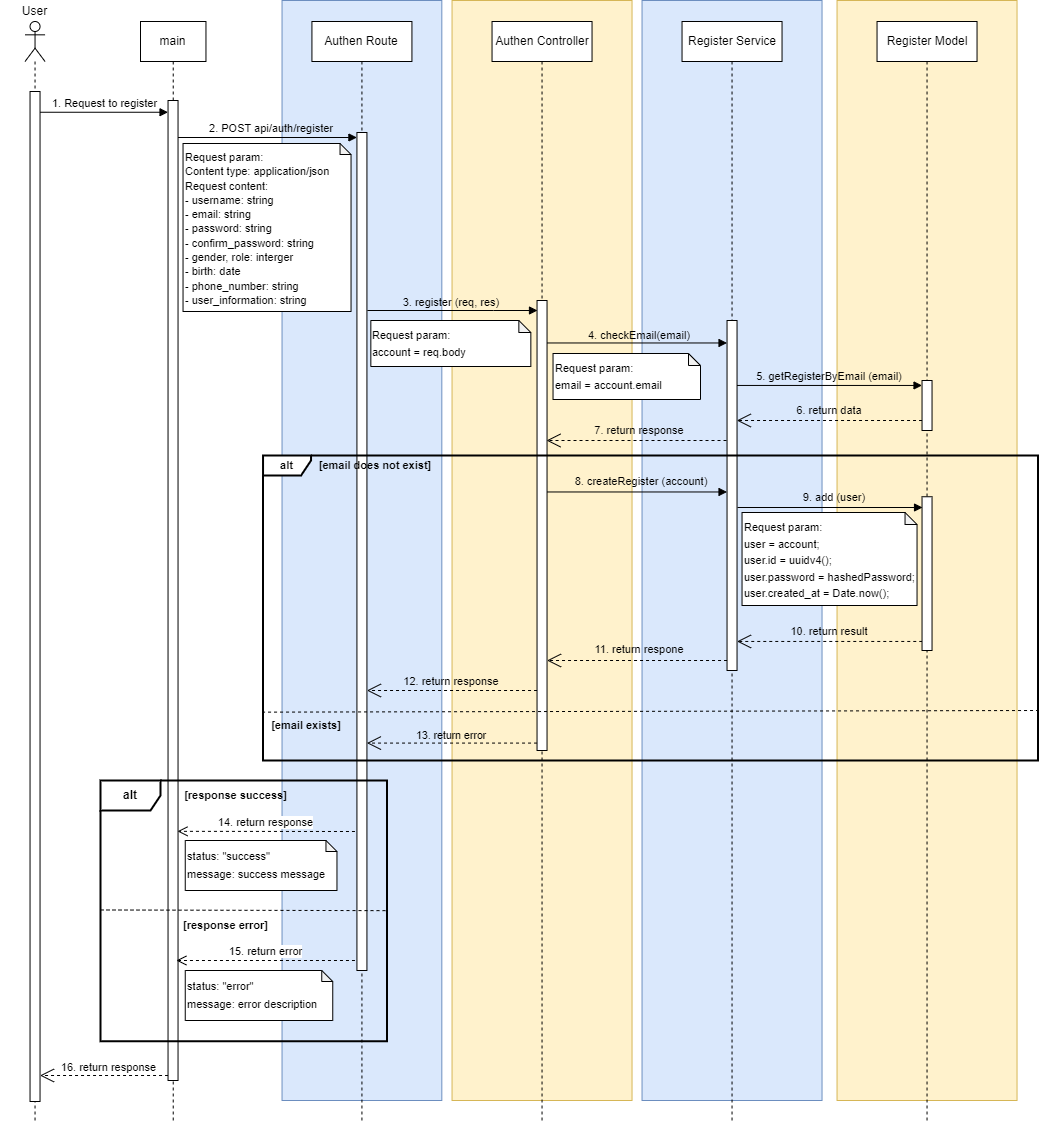
\includegraphics[scale=0.4]{Images/sequence_api/register.png}
  \caption[Sơ đồ tuần tự cho API đăng ký tài khoản vào hệ thống]{\bfseries \fontsize{12pt}{0pt}
  \selectfont Sơ đồ tuần tự cho API đăng ký tài khoản vào hệ thống }
  \label{api_register} %đặt tên cho ảnh
\end{figure}
Hình \ref{api_register} phân tích luồng thông tin người dùng đăng ký tài khoản trên hệ thống. Người dùng gửi yêu cầu đăng ký, yêu cầu được xử lý bởi AuthenController. AuthenController kiểm tra thông tin người dùng qua RegisterService, 
nếu thông tin xác minh chính xác, hệ thống sẽ tạo tài khoản phê duyệt trên RegisterModel và trả về thông báo cho người dùng. Ngược lại, nếu có lỗi xảy ra, hệ thống trả về lỗi tương ứng. 

\begin{figure}[H]
  \centering
  \includegraphics[scale=0.3]{Images/sequence_api/login.png}
  \caption[Sơ đồ tuần tự cho API đăng nhập vào hệ thống]{\bfseries \fontsize{12pt}{0pt}
  \selectfont Sơ đồ tuần tự cho API đăng nhập vào hệ thống }
  \label{api_login} %đặt tên cho ảnh
\end{figure}
Hình \ref{api_login}  phân tích luồng thông tin người dùng đăng nhập tài khoản trên hệ thống. Người dùng gửi yêu cầu đăng nhập, yêu cầu được xử lý bởi AuthenController. AuthenController xác minh thông tin người dùng qua AuthenService. Nếu 
thông tin xác minh chính xác,  TokenService tạo token truy cập và token làm mới và trả về kết quả cho người dùng. Ngược lại, nếu có lỗi xảy ra, hệ thống trả về lỗi tương ứng

% ----------------------------------------------


% ------------------------User----------------------


\paragraph{API quản lý thông tin người dùng}
\mbox{}

\begin{figure}[H]
  \centering
  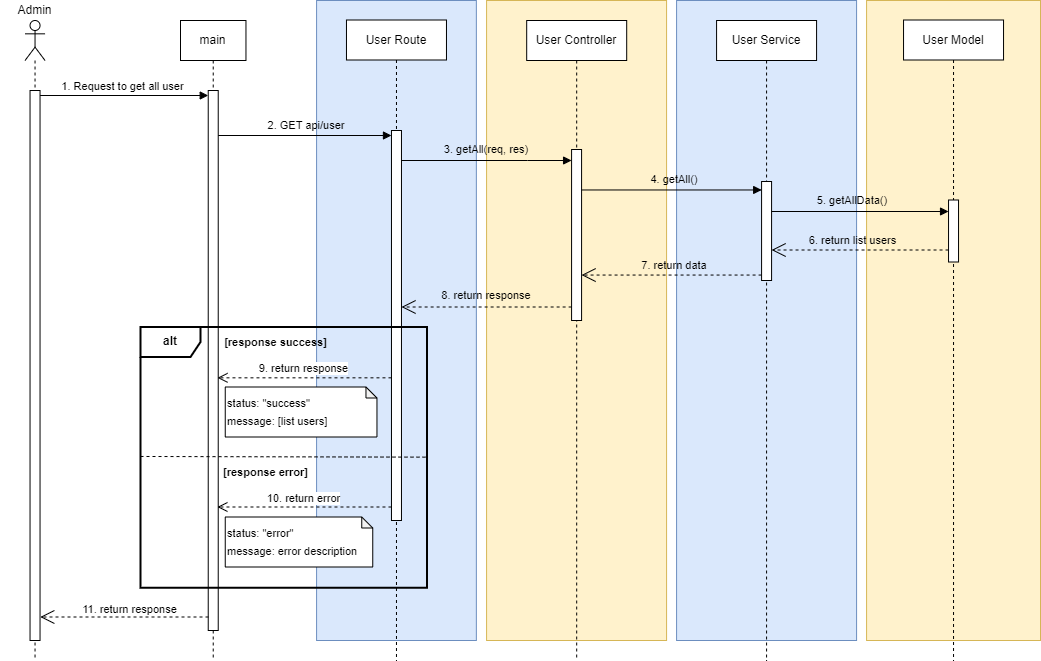
\includegraphics[scale=0.33]{Images/sequence_api/getAllUsers.png}
  \caption[Sơ đồ tuần tự cho API lấy danh sách tất cả người dùng ]{\bfseries \fontsize{12pt}{0pt}
  \selectfont Sơ đồ tuần tự cho API lấy danh sách tất cả người dùng }
  \label{api_getAllUser} %đặt tên cho ảnh
\end{figure}
Hình \ref{api_getAllUser} phân tích luồng thông tin lấy danh sách tất cả người dùng trong hệ thống. Quản trị viên gửi yêu cầu lấy danh sách người dùng, yêu cầu này được xử lý bởi UserController. UserController thông qua User Service gửi truy vấn UserModel để lấy danh sách người dùng . 
Nếu kết quả thành công, hệ thống trả về danh sách người dùng, ngược lại, hệ thống trả về lỗi tương ứng.

% sửa lại ảnh 
\begin{figure}[H]
  \centering
  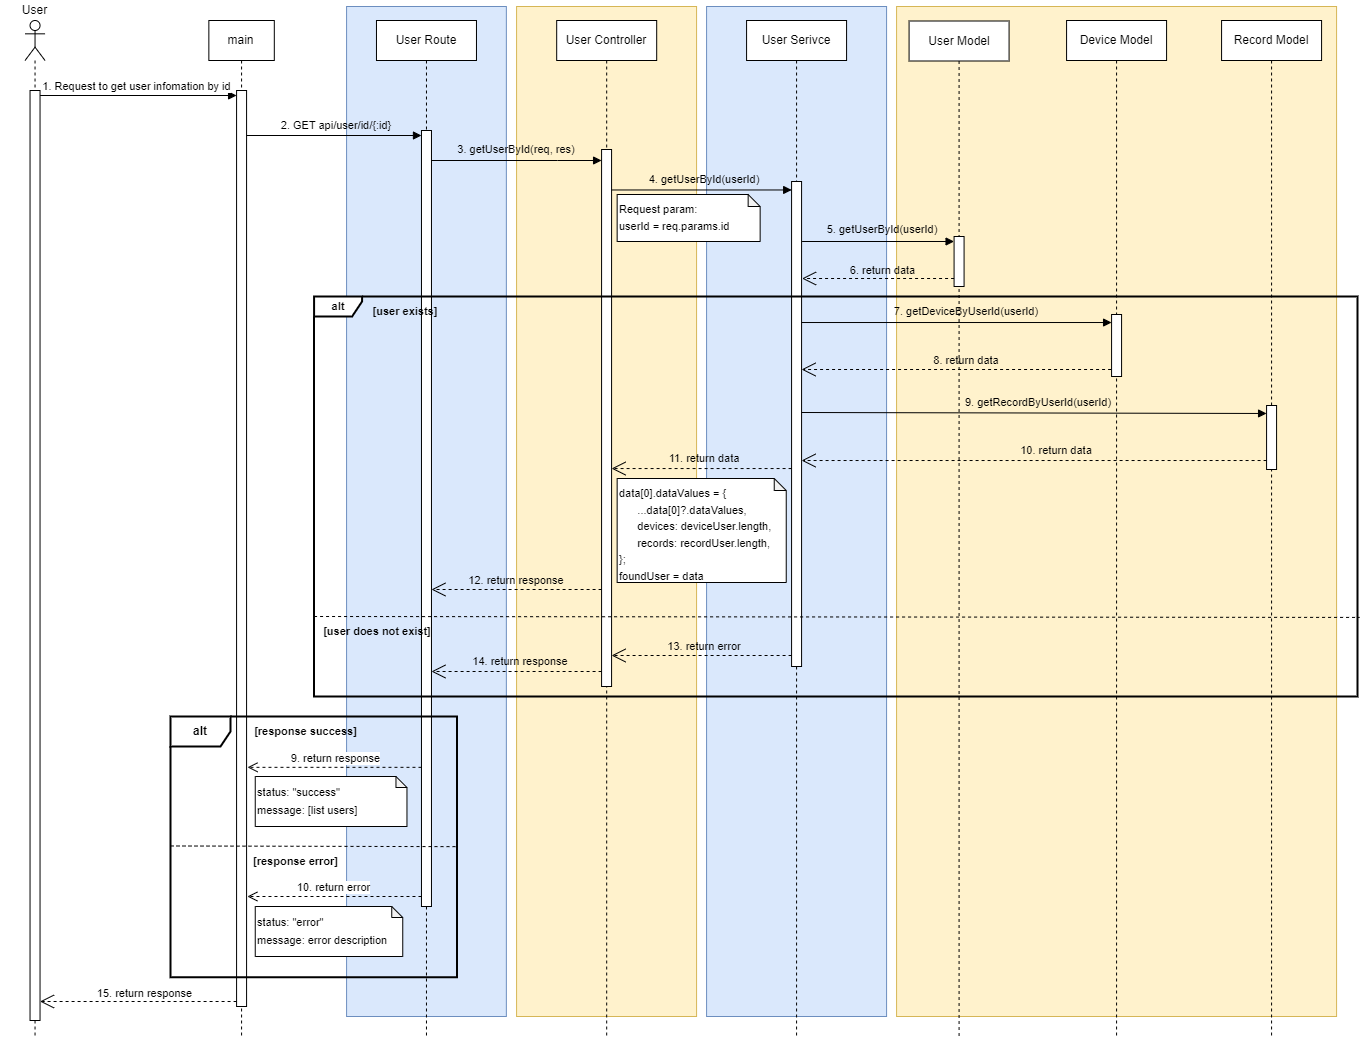
\includegraphics[scale=0.3]{Images/sequence_api/getUserById.png}
  \caption[Sơ đồ tuần tự cho API lấy thông tin của người dùng dựa trên ID ]{\bfseries \fontsize{12pt}{0pt}
  \selectfont Sơ đồ tuần tự cho API lấy thông tin của người dùng dựa trên ID }
  \label{api_getUserById} %đặt tên cho ảnh
\end{figure}
Hình \ref{api_getUserById} phân tích luồng thông tin lấy dữ liệu người dùng theo ID trên hệ thống. Người dùng gửi yêu cầu lấy thông tin người dùng theo ID, yêu cầu này được xử lý bởi UserController. UserController kiểm tra thông tin qua UserService, nếu 
xác minh thông tin có trong hệ thống, UserService sẽ truy vấn UserModel để lấy thông tin người dùng. Nếu truy vấn thành công, hệ thống trả về thông tin người dùng, ngược lại, hệ thống trả về lỗi tương ứng.

\begin{figure}[H]
  \centering
  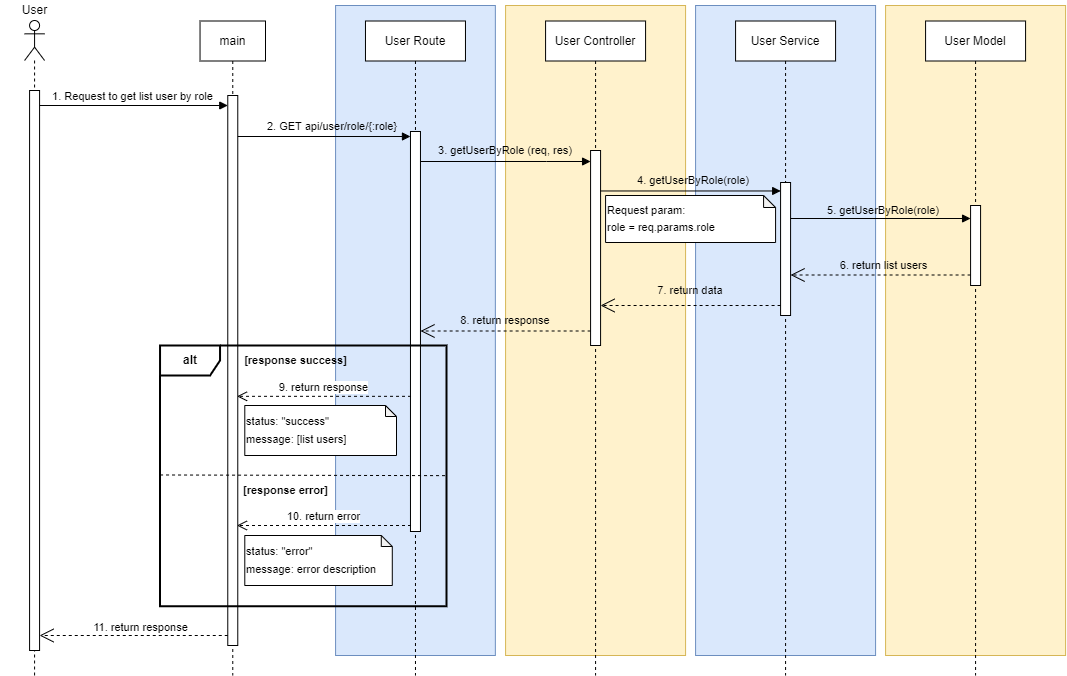
\includegraphics[scale=0.4]{Images/sequence_api/getUserByRole.png}
  \caption[Sơ đồ tuần tự cho API lấy danh sách người dùng dựa theo chức vụ ]{\bfseries \fontsize{12pt}{0pt}
  \selectfont Sơ đồ tuần tự cho API lấy danh sách người dùng dựa theo chức vụ }
  \label{api_getUserByRole} %đặt tên cho ảnh
\end{figure}
Hình \ref{api_getUserByRole} phân tích luồng thông tin lấy danh sách dữ liệu người dùng dựa theo chức vụ trong hệ thống. Người dùng gửi yêu cầu lấy danh sách người dùng theo chức vụ, yêu cầu này được xử lý bởi UserController. UserController kiểm tra thông tin qua UserService. nếu thông tin 
chức vụ có trong hệ thống, UserService truy vấn UserModel để lấy danh sách người dùng. Nếu kết quả thành công, hệ thống trả về danh sách người dùng theo chức vụ, ngược lại, hệ thống trả về lỗi tương ứng.

\begin{figure}[H]
  \centering
  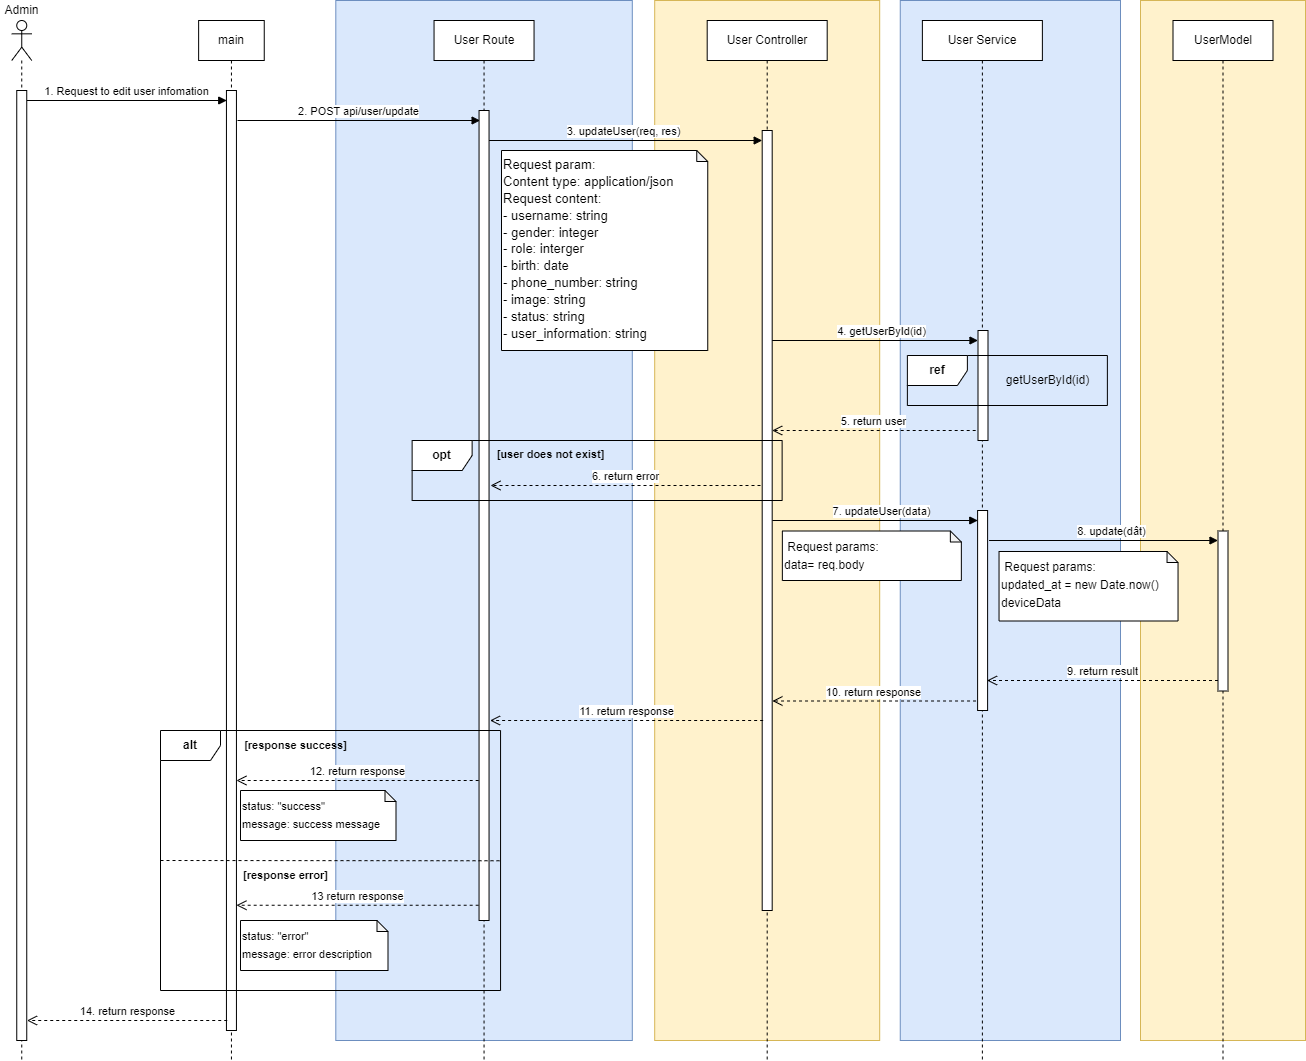
\includegraphics[scale=0.35]{Images/sequence_api/editUser.png}
  \caption[Sơ đồ tuần tự cho API cập nhật thông tin người dùng ]{\bfseries \fontsize{12pt}{0pt}
  \selectfont Sơ đồ tuần tự cho API cập nhật thông tin người dùng }
  \label{api_updateUserById} %đặt tên cho ảnh
\end{figure}
Hình \ref{api_updateUserById} phân tích luồng thông tin cập nhật dữ liệu người dùng trong hệ thống. Người dùng gửi yêu cầu cập nhật thông tin người dùng, 
yêu cầu này được xử lý bởi UserController. UserController gửi truy vấn đến UserService để kiểm tra thông tin người dùng trong hệ thống dựa theo id (ID của người dùng) được truyền vào từ yêu cầu. 
Nếu không tồn tại người dùng, hệ thống sẽ trả về lỗi tương ứng, ngược lại, UserService gửi truy vấn đến UserModel để cập nhật thông tin người dùng. Nếu kết quả thành công, hệ thống trả về kết quả cập nhật cho người dùng, ngược lại, hệ thống trả về lỗi tương ứng.
\begin{figure}[H]
  \centering
  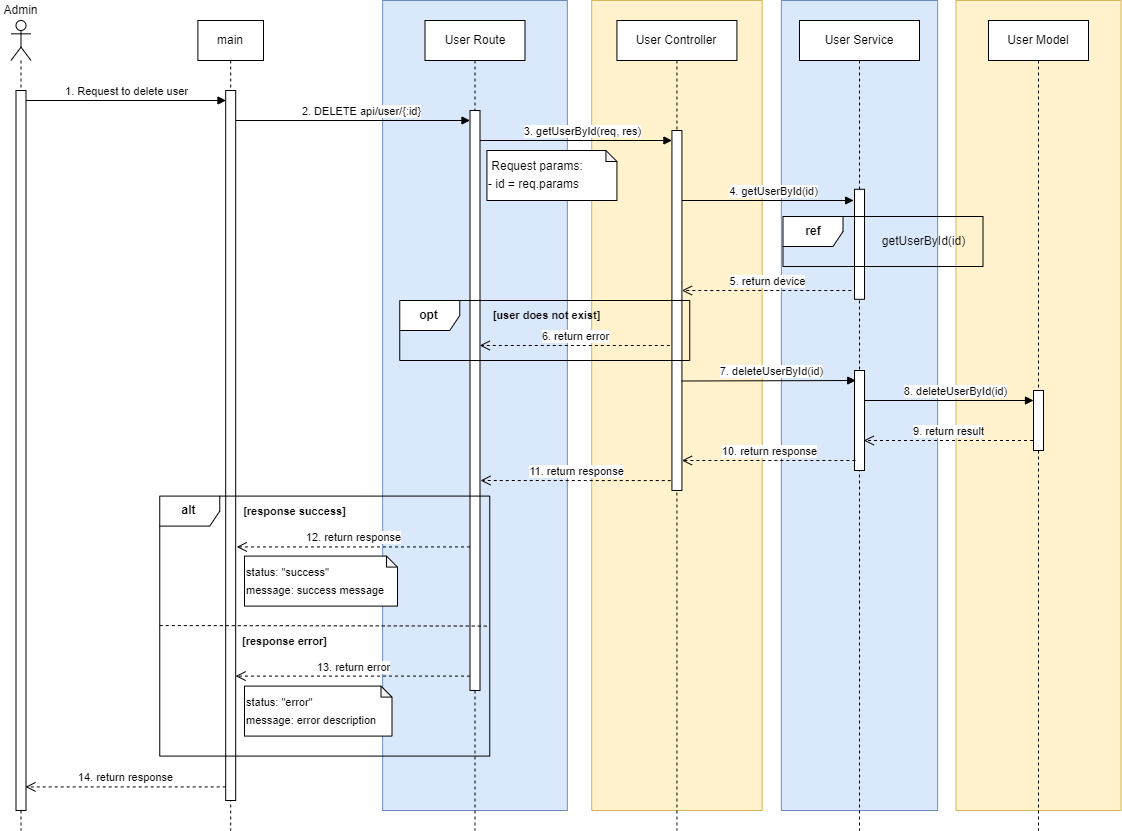
\includegraphics[scale=0.4]{Images/sequence_api/deleteUserById.png}
  \caption[Sơ đồ tuần tự cho API xóa thông tin người dùng ]{\bfseries \fontsize{12pt}{0pt}
  \selectfont Sơ đồ tuần tự cho API xóa thông tin người dùng }
  \label{api_deleteUser} %đặt tên cho ảnh
\end{figure}
Hình \ref{api_deleteUser} phân tích luồng thông tin xóa dữ liệu người dùng trong hệ thống. Quản trị viên gửi yêu cầu xóa dữ liệu người dùng, 
yêu cầu này được xử lý bởi UserController. UserController gửi truy vấn đến UserService để kiểm tra thông tin người dùng trong hệ thống dựa theo id (ID của người dùng) được truyền vào từ yêu cầu. 
Nếu thông tin người dùng không có trong hệ thống, hệ thống sẽ trả về lỗi tương ứng, ngược lại, UserService gửi truy vấn đến UserModel để xóa thông tin người dùng. Sau đó, kết quả cập nhật được trả về 
từ UserModel và được gửi trở lại UserRoute để trả về cho người dùng. Nếu kết quả thành công, hệ thống trả về kết quả cho quản trị viên, ngược lại, hệ thống trả về lỗi tương ứng.

% \linebreak

% ----------------------------------------------

% -------------------------ECG----------------------------
\paragraph{API quản lý bản ghi ECG}
\mbox{}

\begin{figure}[H]
  \centering
  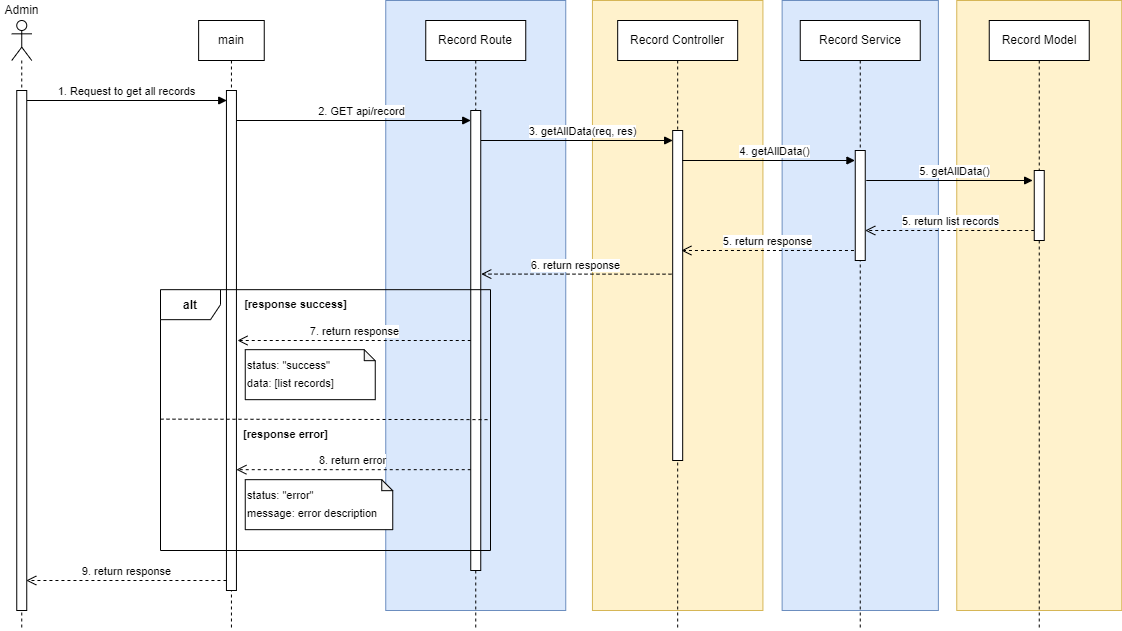
\includegraphics[scale=0.35]{Images/sequence_api/getAllRecord.png}
  \caption[Sơ đồ tuần tự cho API lấy danh sách tất cả phiên đo ECG ]{\bfseries \fontsize{12pt}{0pt}
  \selectfont Sơ đồ tuần tự cho API lấy danh sách tất cả phiên đo ECG }
  \label{api_getAllEcgRecords} %đặt tên cho ảnh
\end{figure}
Hình \ref{api_getAllEcgRecords} phân tích luồng thông tin lấy danh sách dữ liệu tất cả phiên đo ECG (Electrocardiogram) của bệnh nhân trong hệ thống. Quản trị viên gửi yêu cầu lấy danh sách phiên đo ECG của tất cả bệnh nhân, 
yêu cầu này được xử lý bởi RecordController. RecordService gửi yêu cầu qua RecordService, tiếp đó truy vấn đến RecordModel để lấy danh sách dữ liệu ECG. Nếu kết quả thành công, hệ thống trả về danh sách phiên đo, 
ngược lại, hệ thống trả về lỗi tương ứng.

\begin{figure}[H]
  \centering
  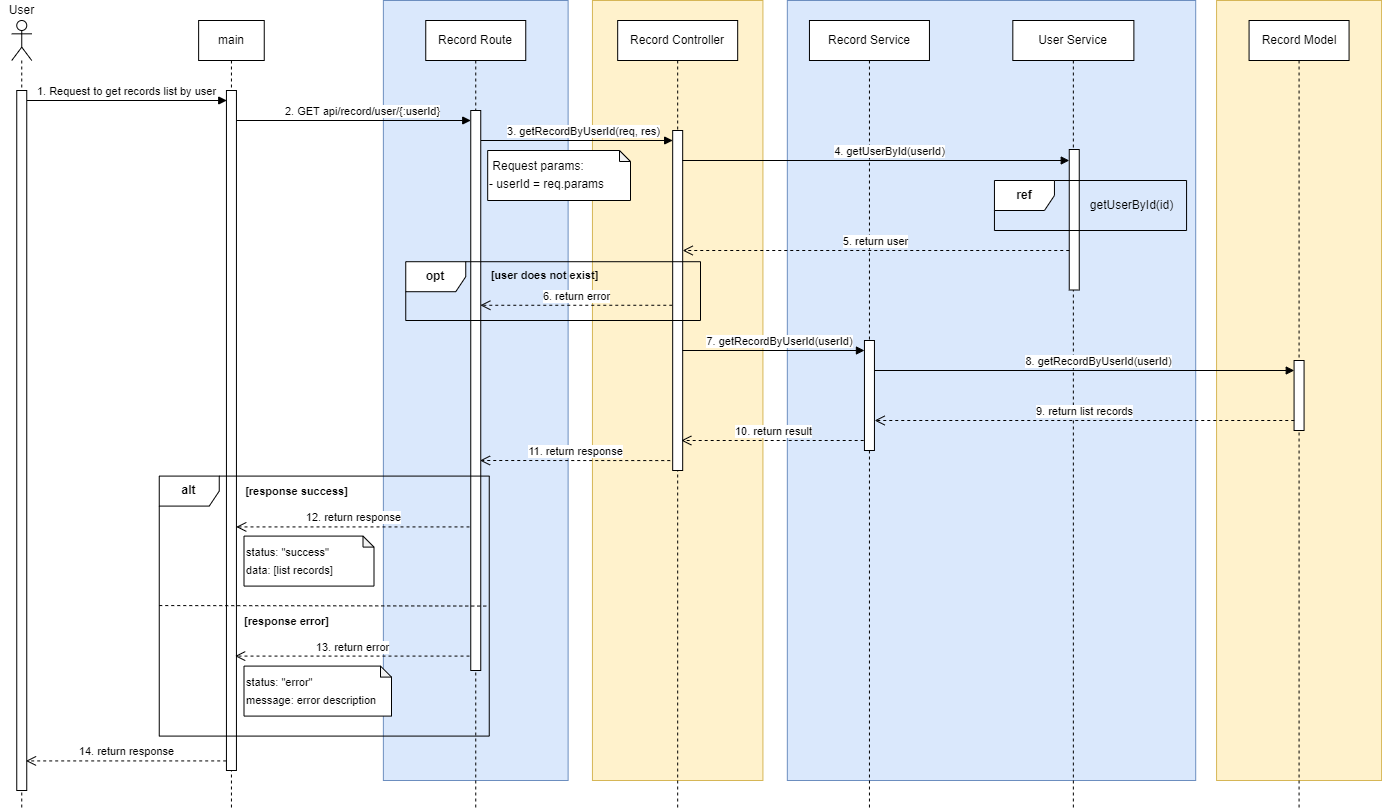
\includegraphics[scale=0.3]{Images/sequence_api/getRecordsByUser.png}
  \caption[Sơ đồ tuần tự cho API lấy danh sách phiên đo ECG của một bệnh nhân ]{\bfseries \fontsize{12pt}{0pt}
  \selectfont Sơ đồ tuần tự cho API lấy danh sách phiên đo ECG của một bệnh nhân }
  \label{api_getRecordsByUser} %đặt tên cho ảnh
\end{figure}
Hình \ref{api_getRecordsByUser} phân tích luồng thông tin lấy danh sách các phiên đo ECG (Electrocardiogram) của một bệnh nhân trong hệ thống. Người dùng gửi yêu cầu lấy danh sách các phiên đo ECG của bệnh nhân, 
yêu cầu này được xử lý bởi RecordController. RecordController gửi truy vấn đến UserService để kiểm tra thông tin bệnh nhân có tồn tại trong hệ thống dựa theo userId (ID của bệnh nhân) được truyền vào từ yêu cầu. Nếu thông tin bệnh nhân ứng vơi ID không có trong hệ thống, hệ thống sẽ
trả về lỗi tương ứng. Ngược lại, RecordService gửi truy vấn đến RecordModel để lấy danh sách dữ liệu ECG dựa trên userId (ID của bệnh nhân) được truyền vào từ yêu cầu. 
Nếu kết quả thành công, hệ thống trả về danh sách phiên đo của bệnh nhân, ngược lại, hệ thống trả về lỗi tương ứng.

 \begin{figure}[H]
  \centering
  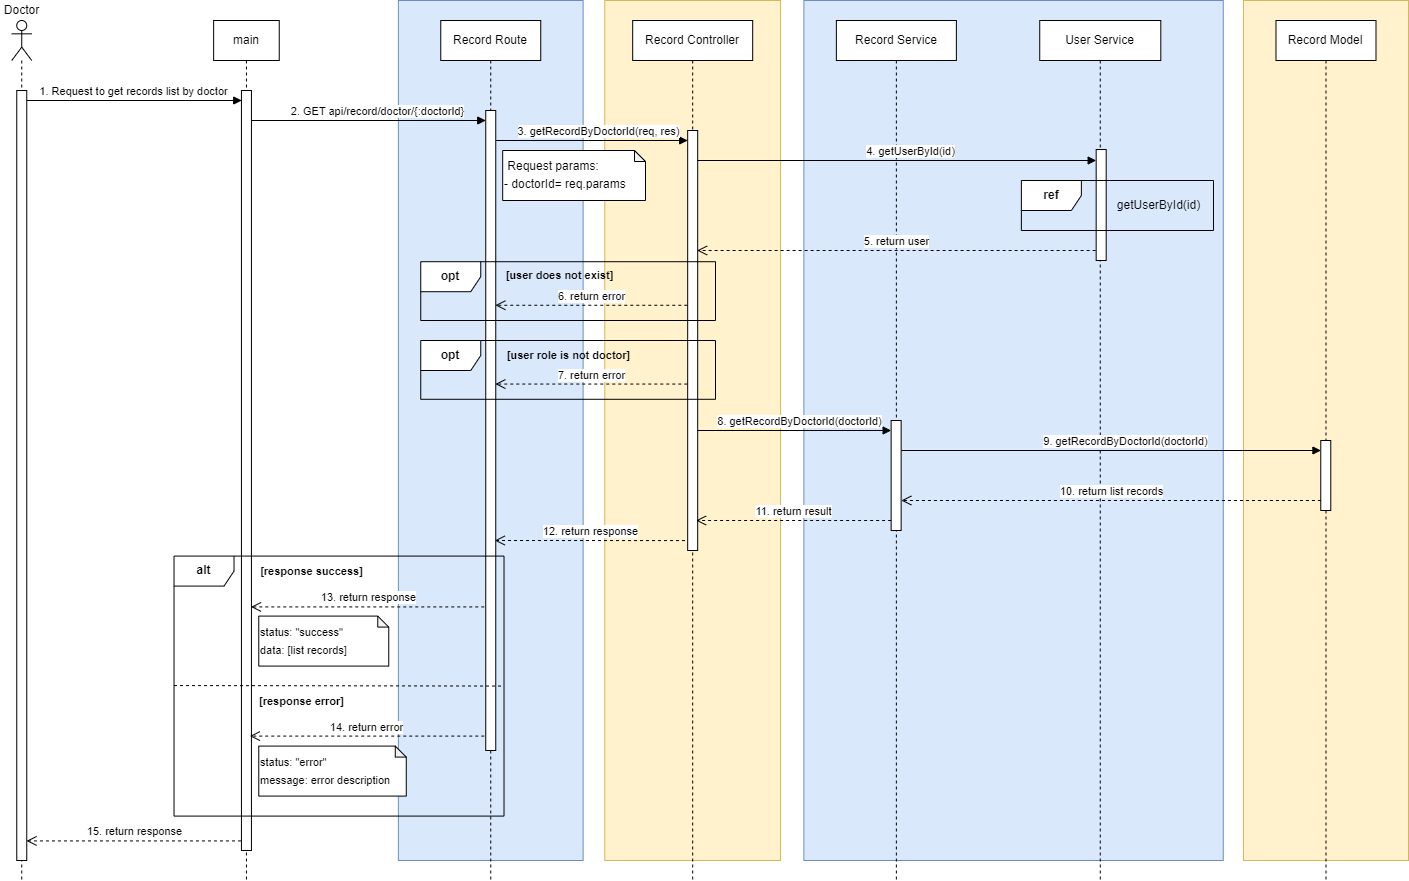
\includegraphics[scale=0.3]{Images/sequence_api/getRecordsByDoctor.png}
  \caption[Sơ đồ tuần tự cho API lấy danh sách phiên đo ECG của bệnh nhân được quản lý bởi một bác sĩ ]{\bfseries \fontsize{12pt}{0pt}
  \selectfont Sơ đồ tuần tự cho API lấy danh sách phiên đo ECG của bệnh nhân được quản lý bởi một bác sĩ}
  \label{api_getRecordsByDoctor} %đặt tên cho ảnh
\end{figure}
Hình \ref{api_getRecordsByDoctor} phân tích luồng thông tin lấy danh sách dữ liệu các phiên đo ECG (Electrocardiogram) của bệnh nhân được quản lý bởi một bác sĩ trong hệ thống. Người dùng gửi yêu cầu lấy danh sách các phiên đo ECG của bệnh nhân được quản lý bởi một bác sĩ, 
yêu cầu này được xử lý bởi RecordController. RecordController gửi truy vấn đến UserService để kiểm tra thông tin bác sĩ có tồn tại trong hệ thống dựa theo doctorId (ID của bác sĩ) được truyền vào từ yêu cầu. Nếu hệ thống không có bác sĩ hay người dùng không phải là bác sĩ, hệ thống sẽ
trả về response lỗi tương ứng. Nếu hệ thồng không có thông tin bác sĩ, RecordService gửi truy vấn đến RecordModel để lấy danh sách dữ liệu ECG dựa trên doctorId (ID của bác sĩ) được truyền vào từ yêu cầu. 
Nếu kết quả thành công, hệ thống trả về danh sách phiên đo của bệnh nhân do bác sĩ phụ trách, ngược lại, hệ thống trả về lỗi tương ứng.

\begin{figure}[H]
  \centering
  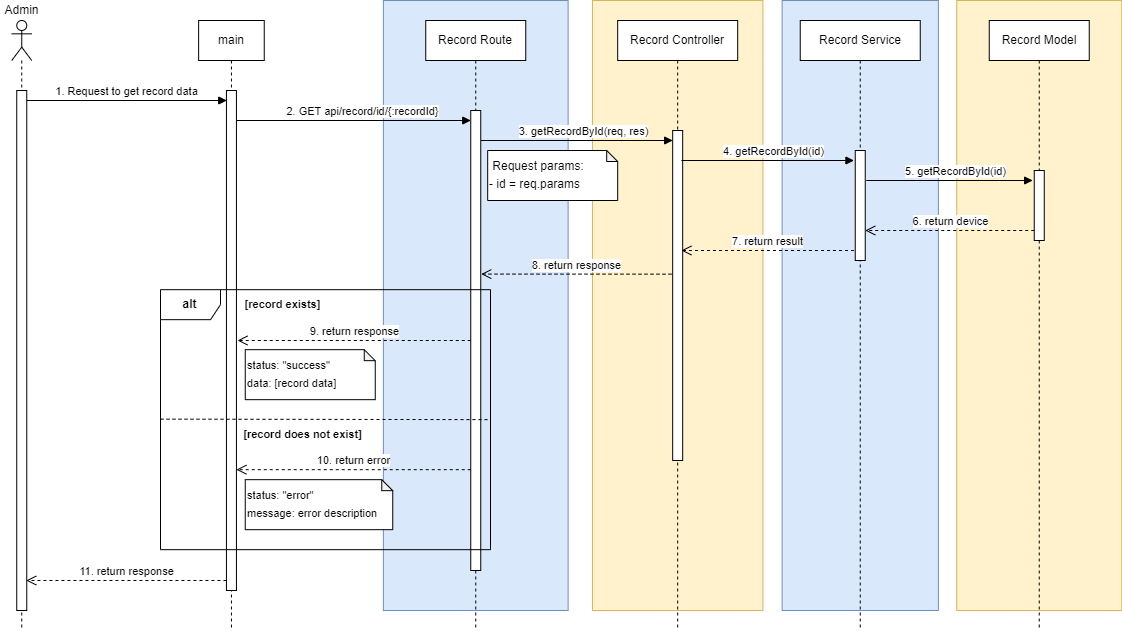
\includegraphics[scale=0.35]{Images/sequence_api/getRecordById.png}
  \caption[Sơ đồ tuần tự cho API lấy thông tin một phiên đo ECG ]{\bfseries \fontsize{12pt}{0pt}
  \selectfont Sơ đồ tuần tự cho API lấy thông tin một phiên đo ECG }
  \label{api_getRecordById} %đặt tên cho ảnh
\end{figure}
Hình \ref{api_getRecordById} phân tích luồng thông tin lấy thông tin một phiên đo ECG (Electrocardiogram) của bệnh nhân trong hệ thống. Người dùng gửi yêu cầu lấy thông tin một phiên đo ECG, 
yêu cầu này được xử lý bởi RecordController. RecordService gửi truy vấn đến RecordModel để lấy thông tin dữ liệu ECG dựa trên recordId (ID của phiên đo) được truyền vào từ yêu cầu. 
Nếu kết quả thành công, hệ thống trả về thông tin phiên đo ECG, ngược lại, hệ thống trả về lỗi tương ứng.
 \begin{figure}[H]
  \centering
  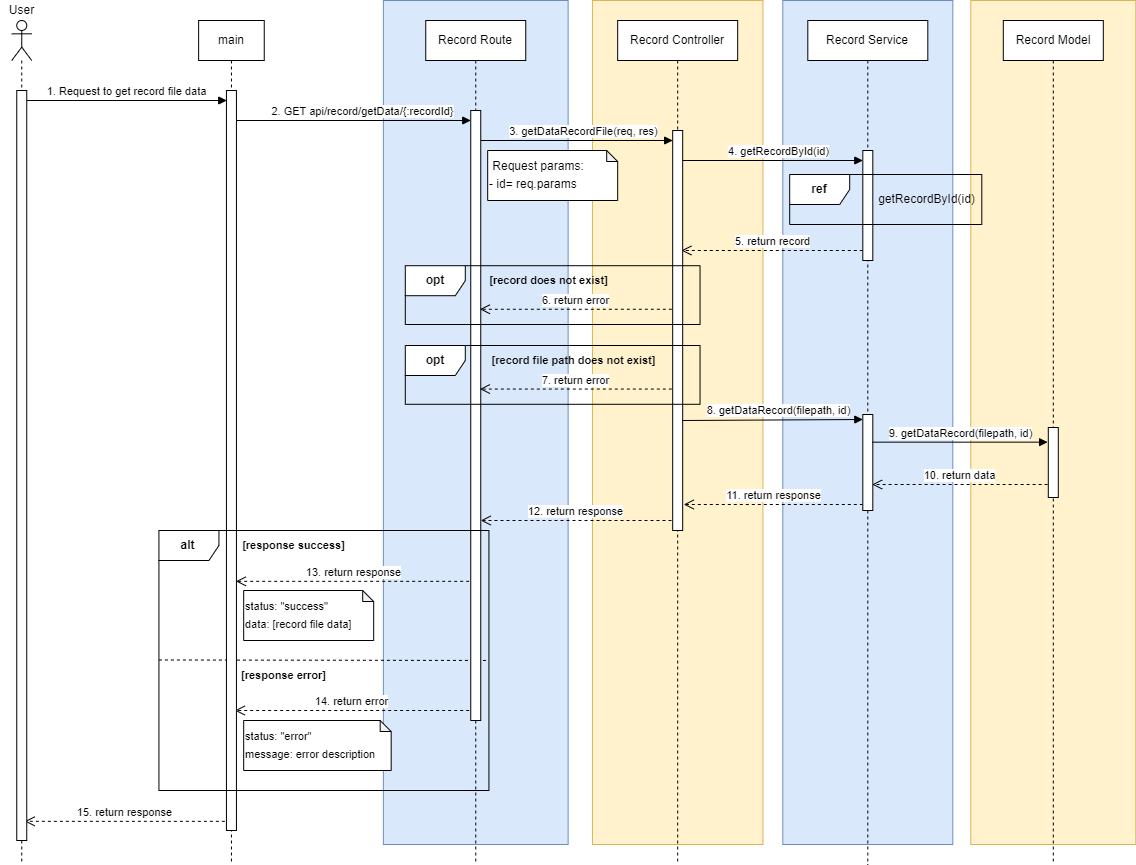
\includegraphics[scale=0.33]{Images/sequence_api/getRecordDataById.png}
  \caption[Sơ đồ tuần tự cho API lấy dữ liệu bản ghi một phiên đo ECG ]{\bfseries \fontsize{12pt}{0pt}
  \selectfont Sơ đồ tuần tự cho API lấy dữ liệu bản ghi một phiên đo ECG }
  \label{api_getRecordDataById} %đặt tên cho ảnh
\end{figure}
Hình \ref{api_getRecordDataById} phân tích luồng thông tin lấy dữ liệu bản ghi một phiên đo ECG (Electrocardiogram) của bệnh nhân trong hệ thống. Người dùng gửi yêu cầu lấy dữ liệu bản ghi một phiên đo của bệnh nhân, 
yêu cầu này được xử lý bởi RecordController. RecordController gửi truy vấn đến RecordService để kiểm tra thông tin, đường dẫn bản ghi có tồn tại trong hệ thống dựa theo recordId (ID của phiên đo) được truyền vào từ yêu cầu. Nếu hệ thống không có thông tin phiên đo hay đường dẫn bản ghi, hệ thống sẽ
trả về lỗi tương ứng. Nếu bản ghi có trong hệ thống, RecordService gửi truy vấn đến RecordModel để lấy dữ liệu ECG dựa trên recordId (ID của phiên đo) được truyền vào từ yêu cầu. 
Nếu kết quả thành công, hệ thống trả về dữ liệu bản ghi phiên đo, ngược lại, hệ thống trả về lỗi tương ứng.

 \begin{figure}[H]
  \centering
  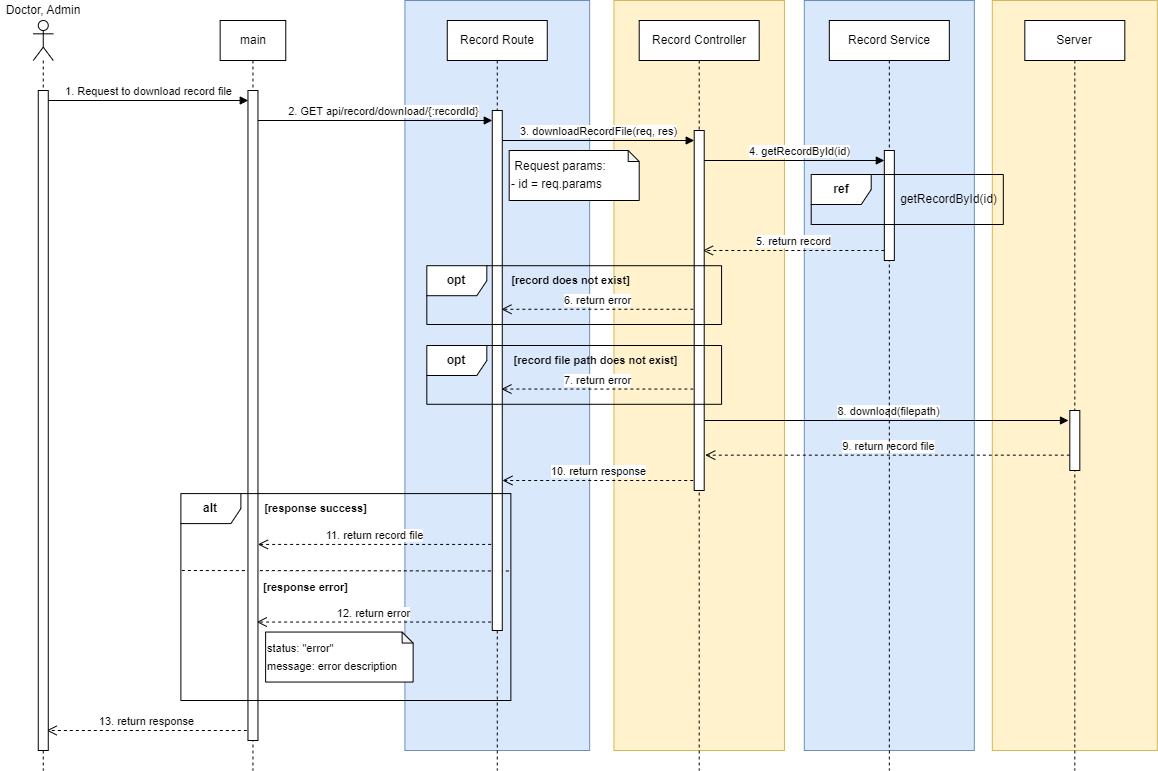
\includegraphics[scale=0.38]{Images/sequence_api/downloadRecordDataById.png}
  \caption[Sơ đồ tuần tự cho API tải tệp bản ghi một phiên đo ECG ]{\bfseries \fontsize{12pt}{0pt}
  \selectfont Sơ đồ tuần tự cho API tải tệp bản ghi một phiên đo ECG }
  \label{api_downloadRecordDataById} %đặt tên cho ảnh
\end{figure}
Hình \ref{api_downloadRecordDataById} phân tích luồng thông tin tải tệp bản ghi một phiên đo của bệnh nhân trong hệ thống. Người dùng gửi yêu cầu tải dữ liệu bản ghi một phiên đo ECG của bệnh nhân, 
yêu cầu này được xử lý bởi RecordController. RecordController gửi truy vấn đến RecordService để kiểm tra thông tin, đường dẫn bản ghi có tồn tại trong hệ thống dựa theo recordId (ID của phiên đo) được truyền vào từ yêu cầu. Nếu hệ thống không có thông tin phiên đo hay đường dẫn bản ghi, hệ thống sẽ
trả về response lỗi tương ứng. Nếu bản ghi có trong hệ thống, RecordService gửi truy vấn đến Server để lấy tệp dữ liệu ECG dựa trên đường dẫn tệp bản ghi được truyền vào từ yêu cầu. 
Nếu kết quả thành công, hệ thống trả về tệp bản ghi của phiên đo, ngược lại, hệ thống trả về lỗi tương ứng.
 \begin{figure}[H]
  \centering
  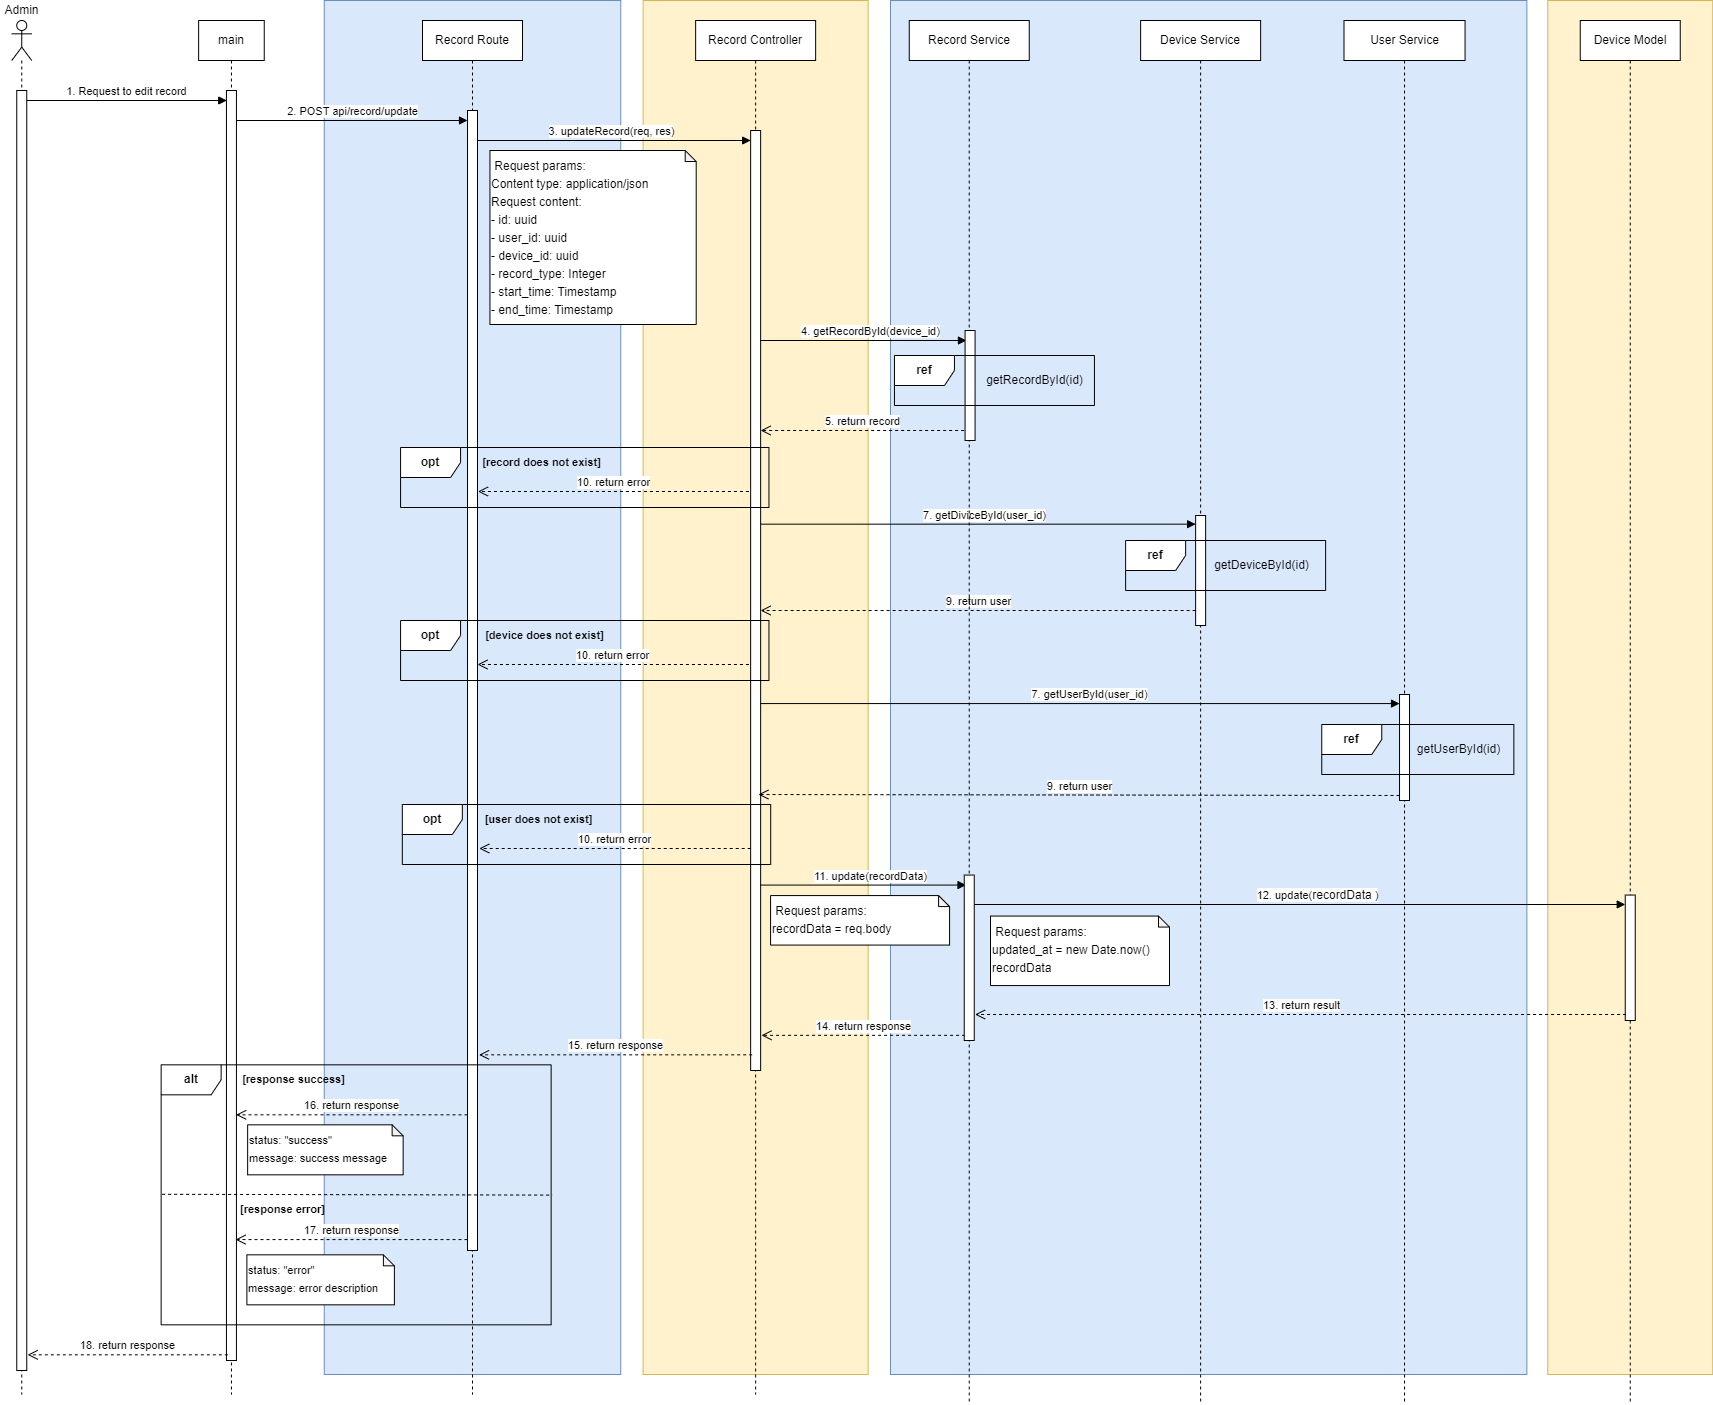
\includegraphics[scale=0.25]{Images/sequence_api/editRecordById.png}
  \caption[Sơ đồ tuần tự cho API cập nhật thông tin một phiên đo ECG ]{\bfseries \fontsize{12pt}{0pt}
  \selectfont Sơ đồ tuần tự cho API cập nhật thông tin một phiên đo ECG }
  \label{api_editRecordById} %đặt tên cho ảnh
\end{figure}
Hình \ref{api_editRecordById} phân tích luồng thông tin cập nhật thông tin một phiên đo ECG (Electrocardiogram) của bệnh nhân trong hệ thống. Người dùng gửi yêu cầu cập nhật thông tin một phiên đo ECG của bệnh nhân, 
yêu cầu này được xử lý bởi RecordController. RecordController gửi truy vấn đến RecordService, DeviceService, UserService để kiểm tra thông tin bản ghi, thiết bị và bệnh nhân trong hệ thống dựa theo id (ID của phiên đo), user\_id (ID của bệnh nhân), device\_id (ID của thiết bị)
 được truyền vào từ yêu cầu. Nếu hệ thống không có thông tin phiên đo, bệnh nhân hay thiết bị, hệ thống sẽ trả về lỗi tương ứng. Nếu thông tin có trong hệ thống, RecordService gửi truy vấn đến RecordModel để cập nhật thông tin
phiên đo ECG dựa trên thông tin được truyền vào từ yêu cầu. Nếu kết quả thành công, hệ thống trả về kết quả cho người dùng, ngược lại, hệ thống trả về lỗi tương ứng.

 \begin{figure}[H]
  \centering
  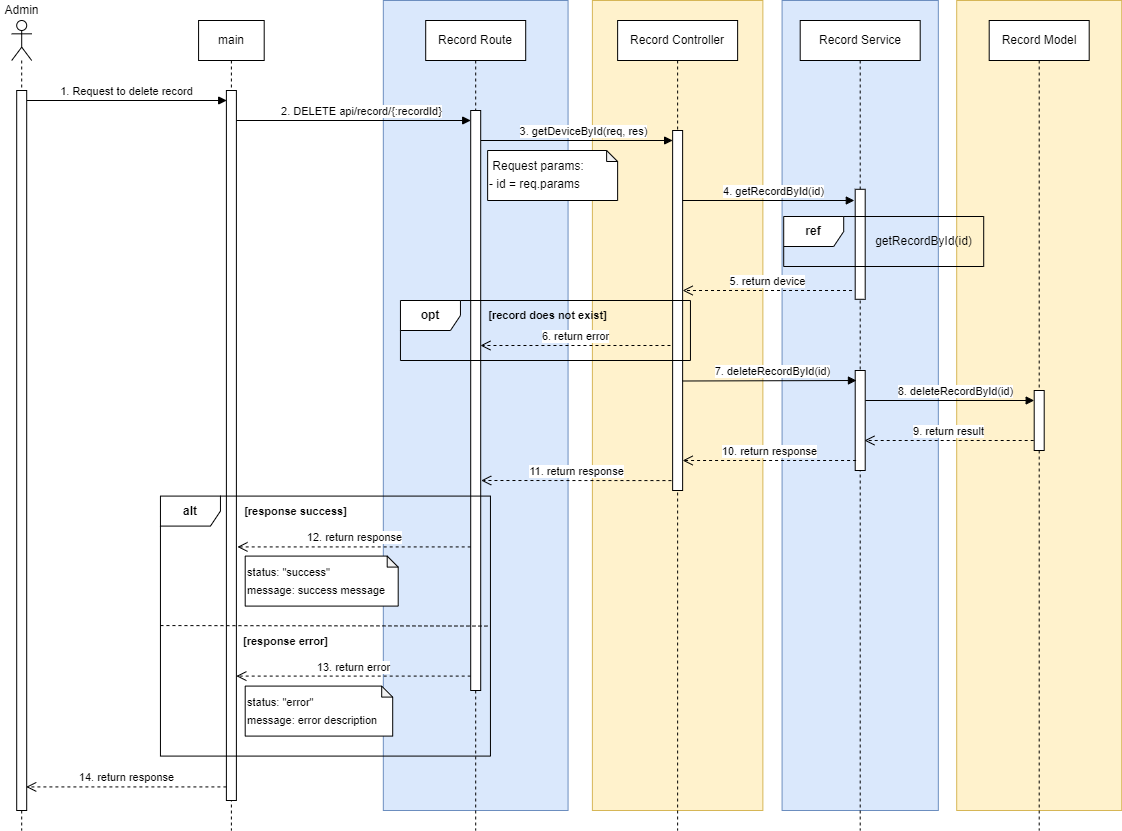
\includegraphics[scale=0.4]{Images/sequence_api/deleteRecordById.png}
  \caption[Sơ đồ tuần tự cho API xóa thông tin một phiên đo ECG ]{\bfseries \fontsize{12pt}{0pt}
  \selectfont Sơ đồ tuần tự cho API xóa thông tin một phiên đo ECG }
  \label{api_deleteRecordById} %đặt tên cho ảnh
\end{figure}
Hình \ref{api_deleteRecordById} phân tích luồng thông tin xóa thông tin một phiên đo ECG (Electrocardiogram) của bệnh nhân trong hệ thống. Người dùng (quản trị viên) gửi yêu cầu xóa thông tin một phiên đo ECG của bệnh nhân,  
yêu cầu này được xử lý bởi RecordController. RecordController gửi truy vấn đến RecordService để kiểm tra thông tin bản ghi trong hệ thống dựa theo recordId (ID của phiên đo) được truyền vào từ yêu cầu.
Nếu thông tin phiên đo có trong hệ thống, RecordService gửi truy vấn đến RecordModel để xóa thông tin phiên đo ECG dựa trên recordId (ID của phiên đo) được truyền vào từ yêu cầu. Nếu kết quả thành công, hệ thống trả về kết quả cập nhật cho người dùng, ngược lại, hệ thống trả về lỗi tương ứng.

% -----------------------------------------------------

% -------------------------Device----------------------------
\paragraph{API quản lý thiết bị}
\mbox{}

\begin{figure}[H]
  \centering
  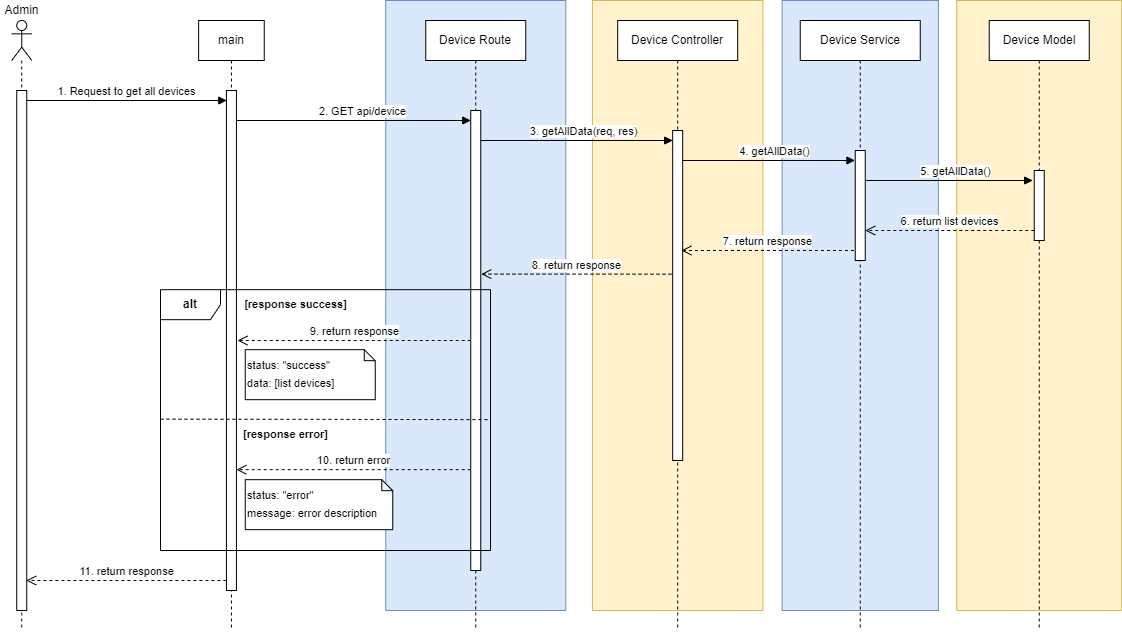
\includegraphics[scale=0.4]{Images/sequence_api/getAllDevices.png}
  \caption[Sơ đồ tuần tự cho API lấy danh sách tất cả thiết bị ]{\bfseries \fontsize{12pt}{0pt}
  \selectfont Sơ đồ tuần tự cho API lấy danh sách tất cả thiết bị }
  \label{api_getAllDevices} %đặt tên cho ảnh
\end{figure}
Hình \ref{api_getAllDevices} phân tích luồng thông tin lấy danh sách tất cả thiết bị trong hệ thống. Quản trị viên gửi yêu cầu lấy danh sách thiết bị, 
yêu cầu này được xử lý bởi DeviceController. DeviceController tiếp tục gửi truy vấn đến DeviceService, DeviceService gửi truy vấn đến DeviceModel 
để lấy danh sách thiết bị. Nếu kết quả thành công, hệ thống trả về danh sách thiết bị trong hệ thống, ngược lại, hệ thống trả về lỗi tương ứng.

\begin{figure}[H]
  \centering
  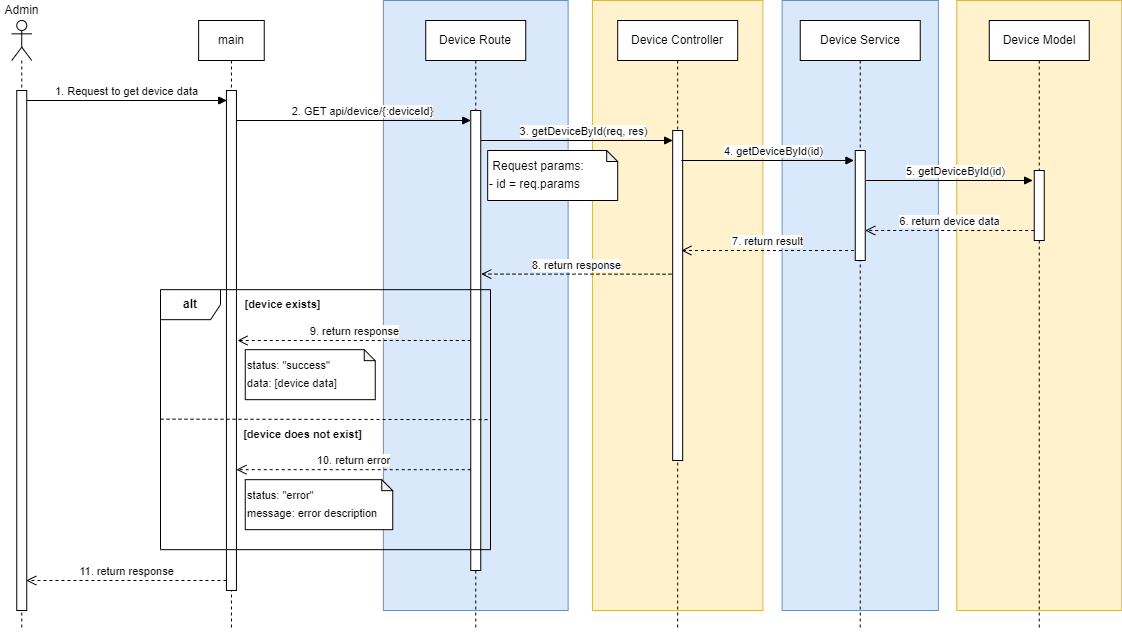
\includegraphics[scale=0.4]{Images/sequence_api/getDeviceById.png}
  \caption[Sơ đồ tuần tự cho API lấy thông tin thiết bị dựa trên ID]{\bfseries \fontsize{12pt}{0pt}
  \selectfont Sơ đồ tuần tự cho API lấy thông tin thiết bị dựa trên ID }
  \label{api_getDeviceById} %đặt tên cho ảnh
\end{figure}
Hình \ref{api_getDeviceById} phân tích luồng thông tin lấy thông tin thiết bị theo ID trên hệ thống. Quản trị viên gửi yêu cầu lấy thông tin thiết bị theo ID, 
yêu cầu này được xử lý bởi DeviceController. DeviceService gửi truy vấn đến DeviceModel để lấy thông tin thiết bị dựa theo deviceId (ID của thiết bị). 
Nếu kết quả thành công, hệ thống trả về thông tin thiết bị, ngược lại, hệ thống trả về lỗi tương ứng.
\begin{figure}[H]
  \centering
  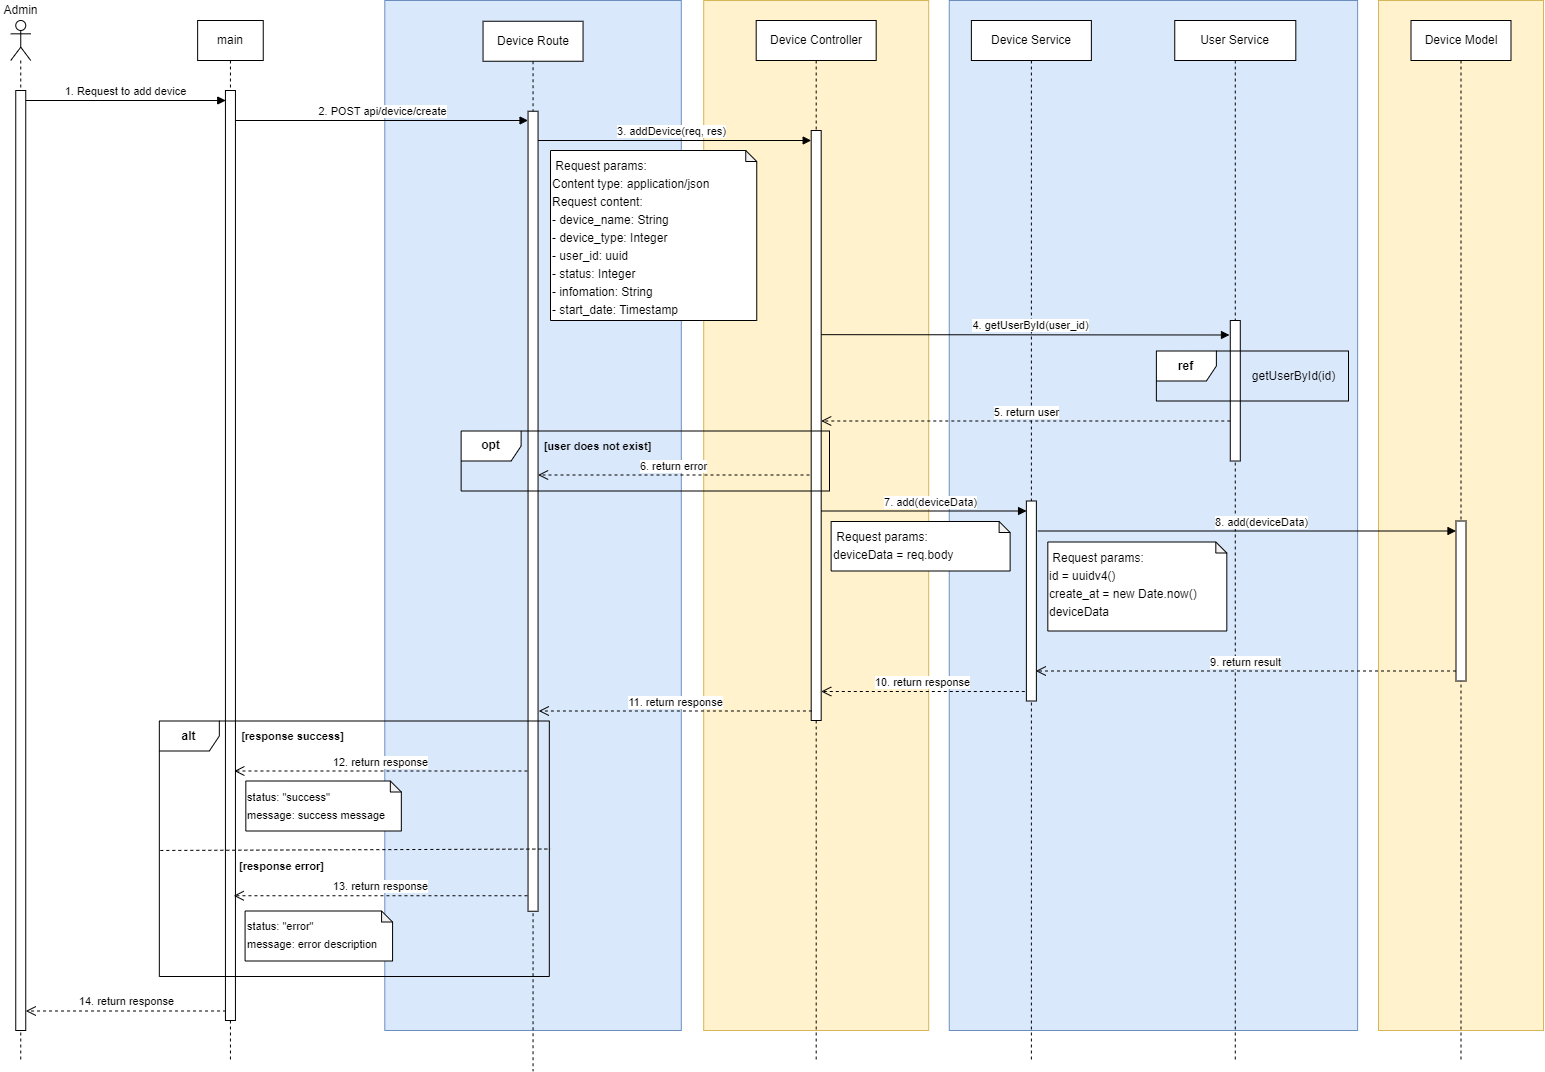
\includegraphics[scale=0.3]{Images/sequence_api/addDevice.png}
  \caption[Sơ đồ tuần tự cho API thêm thiết bị]{\bfseries \fontsize{12pt}{0pt}
  \selectfont Sơ đồ tuần tự cho API thêm thiết bị }
  \label{api_addDevice} %đặt tên cho ảnh
\end{figure}
Hình \ref{api_addDevice} phân tích luồng thông tin thêm thiết bị vào hệ thống. Quản trị viên gửi yêu cầu tạo thông tin thiết bị, 
yêu cầu này được xử lý bởi DeviceController. DeviceController gửi truy vấn đến UserService để kiểm tra thông tin người dùng trong hệ thống dựa theo user\_id (ID của bệnh nhân) được truyền vào từ yêu cầu. 
Nếu bệnh nhân không có trong hệ thống, hệ thống sẽ trả về lỗi tương ứng. Nếu thông tin có trong hệ thống, DeviceService gửi truy vấn đến DeviceModel để thêm thông tin thiết bị 
dựa theo thông tin truyền vào. Nếu kết quả thành công, hệ thống trả về kết quả cho quản trị viên, ngược lại, hệ thống trả về lỗi tương ứng.

\begin{figure}[H]
  \centering
  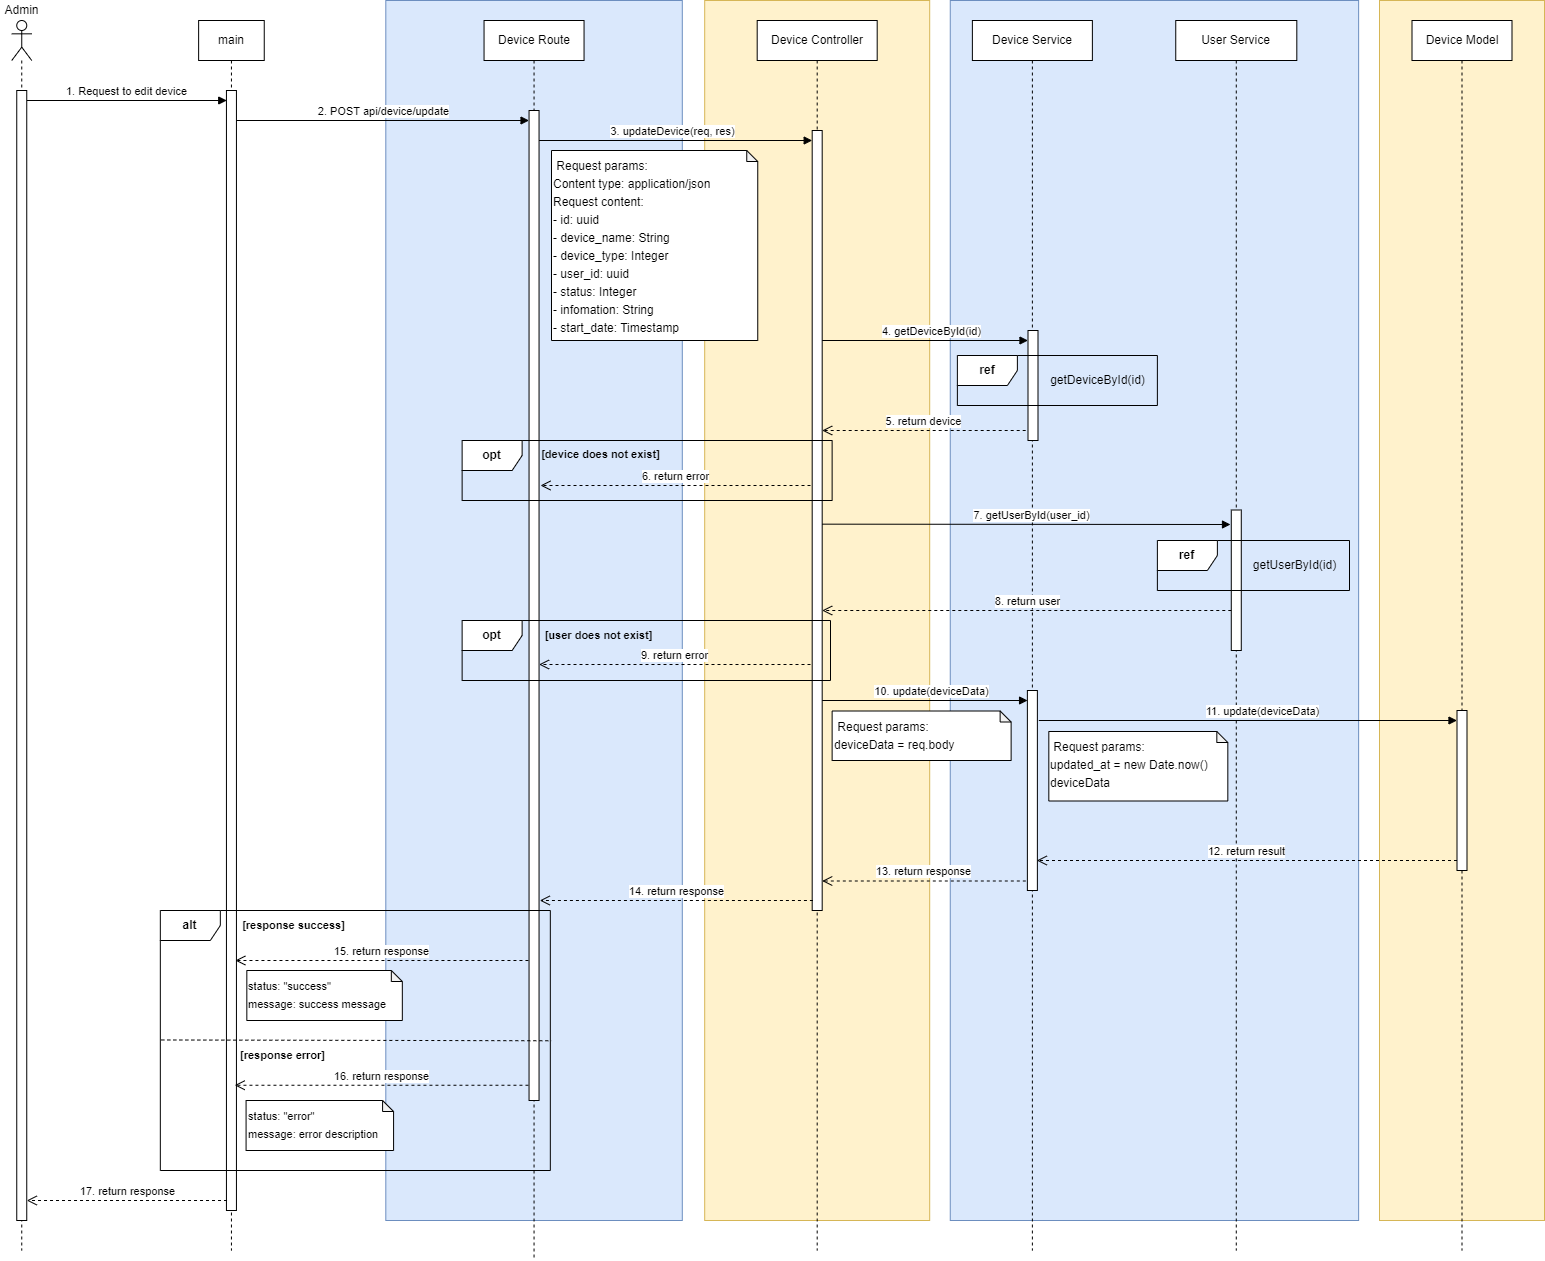
\includegraphics[scale=0.3]{Images/sequence_api/editDevice.png}
  \caption[Sơ đồ tuần tự cho API cập nhật thông tin thiết bị ]{\bfseries \fontsize{12pt}{0pt}
  \selectfont Sơ đồ tuần tự cho API cập nhật thông tin thiết bị }
  \label{api_editDevice} %đặt tên cho ảnh
\end{figure}
Hình \ref{api_editDevice} phân tích luồng thông tin cập nhật thông tin một thiết bị trong hệ thống. Quản trị viên gửi yêu cầu cập nhật thông tin một thiết bị, 
yêu cầu này được xử lý bởi DeviceController. DeviceController gửi truy vấn đến DeviceService, UserService để kiểm tra thông tin thiết bị và bệnh nhân trong hệ thống dựa theo id (ID của thiết bị),
 user\_id (ID của bệnh nhân) được truyền vào từ yêu cầu. Nếu thông tin có trong hệ thống, 
 DeviceService gửi truy vấn đến DeviceModel để cập nhật thông tin thiết bị dựa trên thông tin được truyền vào từ yêu cầu. Nếu kết quả thành công, hệ thống trả về kết quả cập nhật, ngược lại, hệ thống trả về lỗi tương ứng.

 \begin{figure}[H]
  \centering
  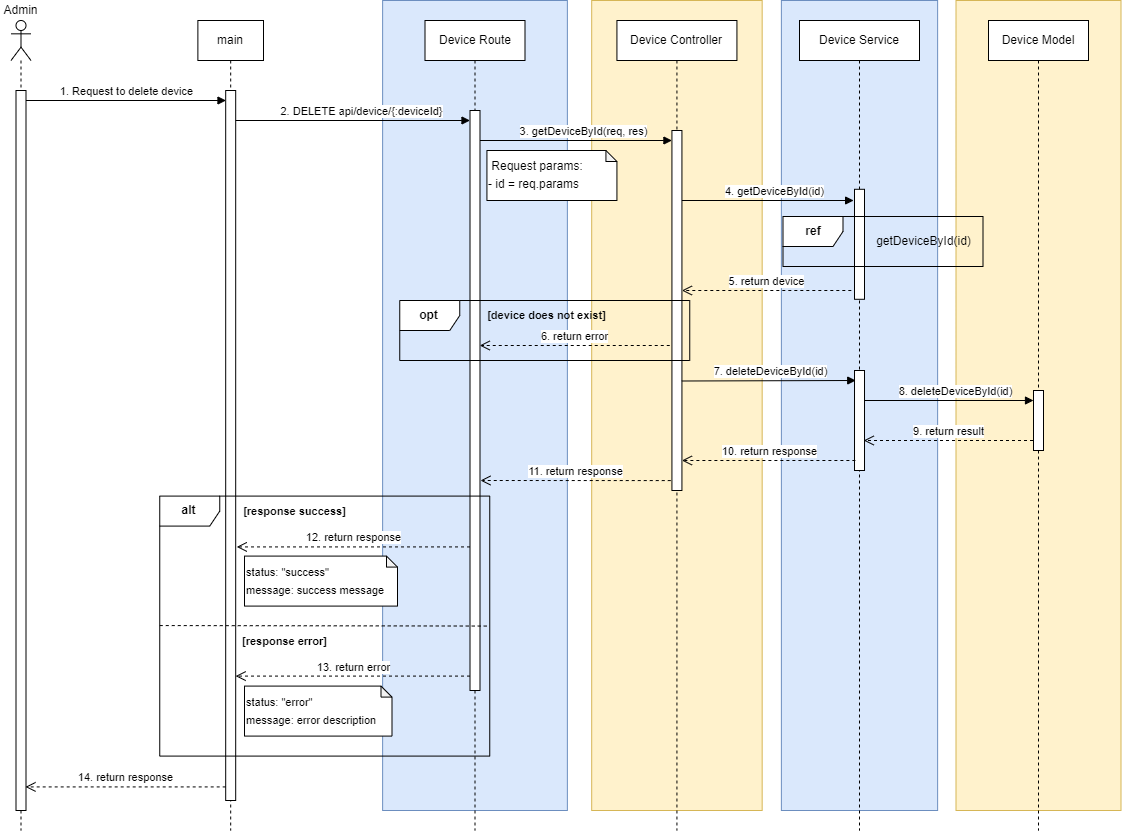
\includegraphics[scale=0.4]{Images/sequence_api/deleteDeviceById.png}
  \caption[Sơ đồ tuần tự cho API xóa thiết bị]{\bfseries \fontsize{12pt}{0pt}
  \selectfont Sơ đồ tuần tự cho API xóa thiết bị }
  \label{api_deleteDeviceById} %đặt tên cho ảnh
\end{figure}
Hình \ref{api_deleteDeviceById} phân tích luồng thông tin xóa thiết bị trong hệ thống. Quản trị viên gửi yêu cầu xóa thông tin thiết bị, 
yêu cầu này được xử lý bởi DeviceController. DeviceController gửi truy vấn đến DeviceService để kiểm tra thông tin thiết bị trong hệ thống dựa theo deviceId (ID của thiết bị) được truyền vào từ yêu cầu. 
Nếu thiết bị có trong hệ thống, DeviceService sẽ gửi truy vấn đến DeviceModel để xóa thông tin thiết bị 
dựa theo thông tin truyền vào. Nếu kết quả thành công, hệ thống trả về kết quả xóa cho quản trị viên, ngược lại, hệ thống trả về lỗi tương ứng.

% -----------------------------------------------------

% -----------------------PatientDoctor------------------------------

\paragraph{API quản lý phân công bác sĩ - bệnh nhân}
\mbox{}


\begin{figure}[H]
  \centering
  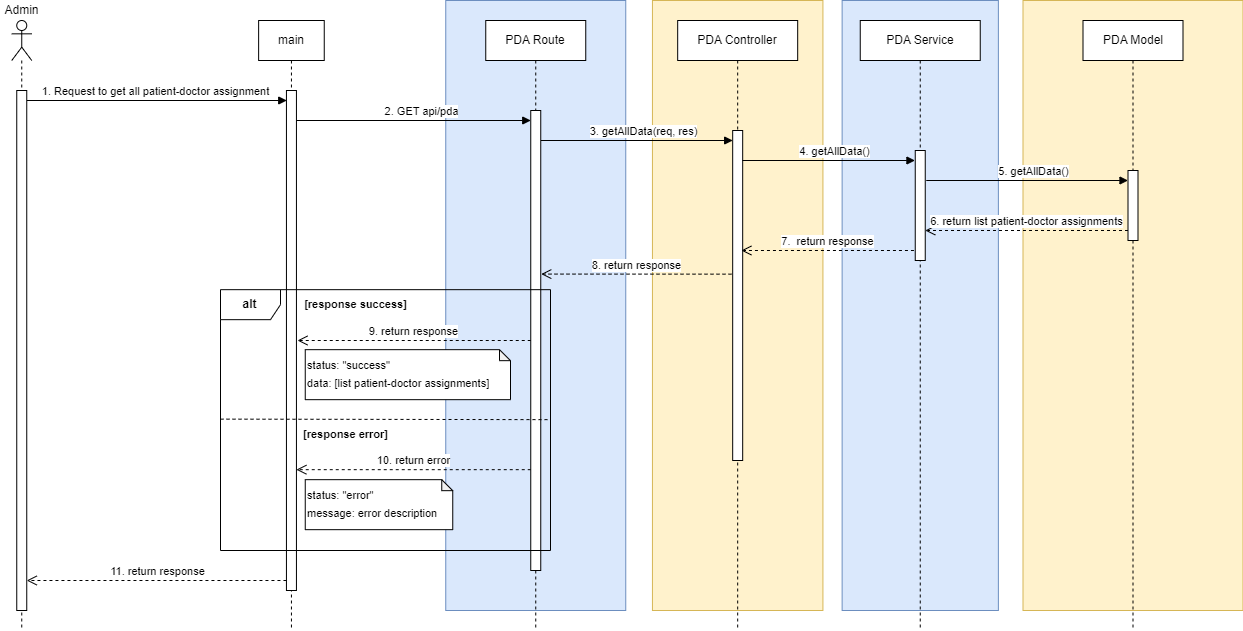
\includegraphics[scale=0.35]{Images/sequence_api/getAllPDA.png}
  \caption[Sơ đồ tuần tự cho API lấy danh sách tất cả phân công bác sĩ - bệnh nhân ]{\bfseries \fontsize{12pt}{0pt}
  \selectfont Sơ đồ tuần tự cho API lấy danh sách tất cả phân công bác sĩ - bệnh nhân }
  \label{api_getAllPDA} %đặt tên cho ảnh
\end{figure}
Hình \ref{api_getAllPDA} phân tích luồng thông tin lấy danh sách tất cả phân công bác sĩ - bệnh nhân trong hệ thống. Quản trị viên gửi yêu cầu lấy danh sách phân công bác sĩ - bệnh nhân, 
yêu cầu này được xử lý bởi PDAController. PDAService gửi truy vấn đến PDAModel để lấy danh sách phân công. Nếu kết quả thành công, hệ thống trả về danh sách phân công bác sĩ - bệnh nhân cho quản trị viên, ngược lại, hệ thống trả về lỗi tương ứng.
\begin{figure}[H]
  \centering
  \includegraphics[scale=0.3]{Images/sequence_api/getPatientByDoctorId.png}
  \caption[Sơ đồ tuần tự cho API lấy danh sách tất cả bệnh nhân phụ trách bởi một bác sĩ ]{\bfseries \fontsize{12pt}{0pt}
  \selectfont Sơ đồ tuần tự cho API lấy danh sách tất cả bệnh nhân phụ trách bởi một bác sĩ }
  \label{api_getPatient} %đặt tên cho ảnh
\end{figure}
Hình \ref{api_getPatient} phân tích luồng thông tin lấy danh sách tất cả bệnh nhân phụ trách bởi một bác sĩ trong hệ thống. Bác sĩ gửi yêu cầu lấy danh sách bệnh nhân mà mình phụ trách, 
yêu cầu này được xử lý bởi PDAController. PDAService gửi truy vấn đến UserModel để lấy danh sách bệnh nhân dựa theo doctor\_id (ID của bác sĩ). Nếu kết quả thành công, hệ thống trả về danh sách bệnh nhân cho bác sĩ, ngược lại, hệ thống trả về lỗi tương ứng.
Sơ đồ tuần tự lấy thông tin bác sĩ phụ trách của một bệnh nhân cũng tương tự như vậy
\begin{figure}[H]
  \centering
  \includegraphics[scale=0.3]{Images/sequence_api/addAssignment.png}
  \caption[Sơ đồ tuần tự cho API thêm phân công bệnh nhân - bác sĩ]{\bfseries \fontsize{12pt}{0pt}
  \selectfont Sơ đồ tuần tự cho API thêm phân công bệnh nhân - bác sĩ }
  \label{api_addPDA} %đặt tên cho ảnh
\end{figure}
Hình \ref{api_addPDA} phân tích luồng thông tin thêm phân công bệnh nhân - bác sĩ vào hệ thống. Quản trị viên gửi yêu cầu tạo phân công bệnh nhân - bác sĩ,  
yêu cầu này được xử lý bởi PDAController. PDAController gửi truy vấn đến UserService để kiểm tra thông tin bệnh nhân, bác sĩ trong hệ thống dựa theo patient\_id (ID của bệnh nhân), doctor\_id (ID bác sĩ);PDAService để kiểm
tra bệnh nhân đã có phân công bác sĩ dựa theo patient\_id được truyền vào từ yêu cầu. Nếu hệ thống không có bệnh nhân, bác sĩ hay bệnh nhân đã có bác sĩ phân công, hệ thống sẽ trả về lỗi tương ứng. 
Ngược lại, PDAService gửi truy vấn đến PDAModel để thêm thông tin phân công dựa theo thông tin truyền vào. Nếu kết quả thành công, hệ thống trả về kết quả thêm phân công, ngược lại, hệ thống trả về lỗi tương ứng.

\begin{figure}[H]
  \centering
  \includegraphics[scale=0.3]{Images/sequence_api/editAssignment.png}
  \caption[Sơ đồ tuần tự cho API cập nhật thông tin phân công bệnh nhân - bác sĩ]{\bfseries \fontsize{12pt}{0pt}
  \selectfont Sơ đồ tuần tự cho API cập nhật thông tin phân công bệnh nhân - bác sĩ }
  \label{api_editPDA} %đặt tên cho ảnh
\end{figure}
Hình \ref{api_editPDA} phân tích luồng thông tin cập nhật thông tin phân công bệnh nhân - bác sĩ vào hệ thống. Quản trị viên gửi yêu cầu sửa thông tin phân công bệnh nhân - bác sĩ, 
yêu cầu này được xử lý bởi PDAController. PDAController gửi truy vấn đến UserService để kiểm tra thông tin bệnh nhân, bác sĩ trong hệ thống dựa theo patient\_id (ID của bệnh nhân), doctor\_id (ID bác sĩ);PDAService để kiểm
tra bệnh nhân đã có phân công bác sĩ dựa theo patient\_id được truyền vào từ yêu cầu. Nếu hệ thống không có bệnh nhân, bác sĩ hay bệnh nhân chưa có bác sĩ phân công, hệ thống sẽ trả về lỗi tương ứng. 
Ngược lại, PDAService gửi truy vấn đến PDAModel để sửa thông tin phân công dựa theo thông tin truyền vào. Nếu kết quả thành công, hệ thống trả về kết quả cập nhật thông tin phân công bác sĩ - bệnh nhân, ngược lại, hệ thống trả về lỗi tương ứng.

\begin{figure}[H]
  \centering
  \includegraphics[scale=0.4]{Images/sequence_api/deleteAssignment.png}
  \caption[Sơ đồ tuần tự cho API xóa phân công bệnh nhân - bác sĩ]{\bfseries \fontsize{12pt}{0pt}
  \selectfont Sơ đồ tuần tự cho API xóa phân công bệnh nhân - bác sĩ }
  \label{api_deletePDA} %đặt tên cho ảnh
\end{figure}
Hình \ref{api_deletePDA} phân tích luồng thông tin xóa phân công bệnh nhân - bác sĩ trong hệ thống. Quản trị viên gửi yêu cầu xóa thông tin phân công, 
yêu cầu này được xử lý bởi PDAController. PDAController gửi truy vấn đến PDAService để kiểm tra thông tin phân công trong hệ thống dựa theo pdaId (ID của phân công) được truyền vào từ yêu cầu. 
Nếu thông tin có trong hệ thống, PDAService gửi truy vấn đến PDAModel để xóa thông tin phân công 
dựa theo thông tin truyền vào. Nếu kết quả thành công, hệ thống trả về kết quả xóa phân công, ngược lại, hệ thống trả về lỗi tương ứng.
% -----------------------------------------------------
\subsubsection{Chức năng nhắn tin}
Chức năng nhắn tin được thiết kế độc lập với server của hệ thống, có thể tăng khả năng mở rộng, linh hoạt hơn. 
PostgreSQL là nền tảng cơ sở dữ liệu cho chức năng bởi tính phổ biến, hiệu năng cao, hỗ trợ kết nối socket, dễ dàng phát triển cũng như tính bảo mật. PostgreSQL đóng vai trò là trung tâm lưu trữ dữ liệu tin nhắn cho hệ thống nhắn tin, bao gồm bốn bảng chính. 

Các hoạt động liên quan đến tin nhắn như xử lý, gửi và thao tác đều được thực hiện thông qua truy vấn và truy cập trực tiếp vào cơ sở dữ liệu. PostgreSQL cung cấp nhiều
ví dụ và câu lệnh truy vấn sẵn có, giúp việc truy cập và thao tác dữ liệu trở nên dễ dàng và linh hoạt.

\begin{figure}[H]
  \centering
  \includegraphics[width=16cm,height=18cm]{Images/sequence_api/sendGetMessage.png}
  \caption[Sơ đồ tuần tự chức năng gửi và nhận tin nhắn trong hệ thống]{\bfseries \fontsize{12pt}{0pt}
  \selectfont Sơ đồ tuần tự chức năng gửi và nhận tin nhắn trong hệ thống}
  \label{api_sendMessage} %đặt tên cho ảnh
\end{figure}
Hình \ref{api_sendMessage} phân tích luồng thông tin gửi/nhận tin nhắn trên hệ thống. Khi người dùng gửi một tin nhắn qua ChatController, dữ liệu được lưu vào các Model trong CSDL bao gồm Conversation Model, 
Conversation Member Model, Message Model, Message Attachment Model. Ngay sau đó, hệ thống sẽ hiển thị tin nhắn trên màn hội thoại và gửi sang cho người gửi. 
\subsubsection{Chức năng hỏi, nhận tư vấn từ trợ lý ảo}
Chức năng hỏi, nhận tư vấn từ trợ lý ảo giống với chức năng tin, đều được thiết kế để không phụ thuộc vào server của
hệ thống mà sử dụng trợ lý ảo độc lập. Hệ thống lựa chọn OpenAI Model để phát triển
chức năng chat với trợ lý ảo bởi tính phổ biến, hỗ trợ đa ngôn ngữ, dễ sử dụng với tài liệu đầy
đủ và khả năng điều chỉnh linh hoạt. Ở chức năng nhắn tin với trợ lý ảo, mọi dữ liệu về tin nhắn sẽ được lưu tạm thời ở 
server và sẽ mất khi người dùng rời khỏi hệ thống.

Sử dụng mô hình GPT-4 (Generative Pre-trained Transformer) được phát triển bởi OpenAI dựa trên kiến trúc Transformer giúp 
cho tốc độ phản hồi nhanh chóng cùng với đó là cơ chế lưu trữ và học hỏi thông qua các câu hỏi hay câu nhắn tin từ người dùng. 
Qua đó, cải thiện chất lượng, độ chính xác trong phản hồi với người dùng.

\begin{figure}[H]
  \centering
  \includegraphics[width=16cm,height=8cm]{Images/sequence_api/sendMessageChatBot.png}
  \caption[Sơ đồ tuần tự thiết kế chức năng hỏi, nhận tư vấn từ trợ lý ảo]{\bfseries \fontsize{12pt}{0pt}
  \selectfont Sơ đồ tuần tự thiết kế chức năng hỏi, nhận tư vấn từ trợ lý ảo}
  \label{api_sendMessageChatBot} %đặt tên cho ảnh
\end{figure}
Hình \ref{api_sendMessageChatBot} biểu diễn chi tiết cách gửi/nhận tin nhắn cho trợ lý ảo trên hệ thống. Khi người dùng gửi một tin nhắn qua ChatBotController, sau đó sẽ tạo nên cuộc hội thoại mới nếu như người dùng nhắn tin lần đầu. 
Tin nhắn của người dùng sẽ được GPT Model xử lý và trả về tin nhắn phản hồi hiển thị lên màn hình nhắn tin với trợ lý ảo.
\subsection{Kết luận chương}

Chương 3 trình bày chi tiết về quá trình thiết kế hệ thống, bao gồm kiến trúc tổng thể và các thành phần cụ thể. 
Thiết kế hệ thống tập trung vào việc xây dựng kiến trúc vận hành hiệu quả và mượt mà, chú trọng vào tính bảo mật, hiệu suất và khả năng mở rộng tối ưu.
\newpage